%
% Documento: Desenvolvimento
%

\chapter{DESENVOLVIMENTO}

Neste cap\'{i}tulo iremos utilizar \`{a}s teorias do cap\'{i}tulo 2 (Revis\~{a}o liter\'{a}ria) juntamente com as t\'{e}cnicas de Kimball R. e Ross, M. (2013), que se baseiam na modelagem dimensional e iremos teorizar as ferramentas de banco de dados PostgreSQL e Pentaho, para que tenhamos uma base de conhecimento s\'olida em rela\c{c}\~{a}o ao uso e funcionalidades destas ferramentas.

O objetivo deste cap\'{i}tulo \'{e} a implementa\c{c}\~{a}o de um BI/DW, partindo da infraestrutura b\'{a}sica, cria\c{c}\~{a}o do Banco de dados de nome: ``DW\_181'' no PostgreSQL, ETL dos dados de três meses  (janeiro, fevereiro e mar\c{c}o de 2020) de transa\c{c}\~{o}es, provindos do arquivo no formato ``.XLS'' do \textit{Microsoft Excel},  extra\'{i}do do SISGOU, na op\c{c}\~{a}o consulta do disque denúncia, que ser\'{a} processada usando uma das ferramentas do suite Pentaho, o PDI (\textit{Pentaho Data Integration}).

No PDI iremos criar as transforma\c{c}\~{o}es que criaram as tabelas de dimens\~{a}o dentro do Banco de dados, al\'{e}m do PDI iremos demonstrar o uso das outras ferramentas do Pentaho como: PAC (\textit{Pentaho Administration Console}), PUC (\textit{Pentaho User Console}), PSW (\textit{Pentaho schema workbench}) e o PRD (\textit{Pentaho Report Designer}) e finalmente ap\'os os dados serem processados ser\~{a}o armazenados no PostgreSQL, SGBD relacional, onde ficar\'{a} o DW da aplica\c{c}\~{a}o de BI.

\section{Infraestrutura}

A infraestrutura utilizada neste trabalho \'{e} baseada em ferramentas de softwares gratuitos ou \textit{freeware} , da suite de BI ao SGDB relacional, para a base de dados, usamos oPostgreSQL, como dito no t\'opico anterior, juntamente com a Plataforma Pentaho na vers\~{a}o 9.0 \textit{Community} (sem custos), adquirida no site da Hitachi Vantara atualmente \'{e} detentora dos direitos da plataforma e o Java SE \textit{Runtime Environment} vers\~{a}o 1.8.0-151-b12, toda estrutura instalada localmente em um ambiente de desenvolvimento, em um notebook MacBook Pro da Apple (mem\'oria de 16 gb de ram e SSD de 1 Tb), com Sistema Operacional macOS Catalina vers\~{a}o 10.15.6.

\section{SISGOU}

O sistema de processamentos de transa\c{c}\~{o}es de onde se extra\'{i}ram os dados \'{e} o SISGOU, desenvolvidos pelo equipe de TI da SSP/AL, conforme figura abaixo, nele todos os dados das denúncias s\~{a}o registrados pelos atendentes, e ou, denunciantes (via web ou aplicativo), s\~{a}o armazenados em uma base de dados em ORACLE, \'{e} os usu\'{a}rios finais têm acesso apenas pelo menus da aplica\c{c}\~{a}o, em nosso caso m\'odulo ``Aplicativos``, ``disque Denúncia'' e ``Consultar Denúncias``, conforme figura abaixo.

% figuras
\begin{figure}[H]
	\vspace*{0,2cm}
    \centering
    \caption{SISGOU (Sistema de Gerenciamento Operacional Unificado}
    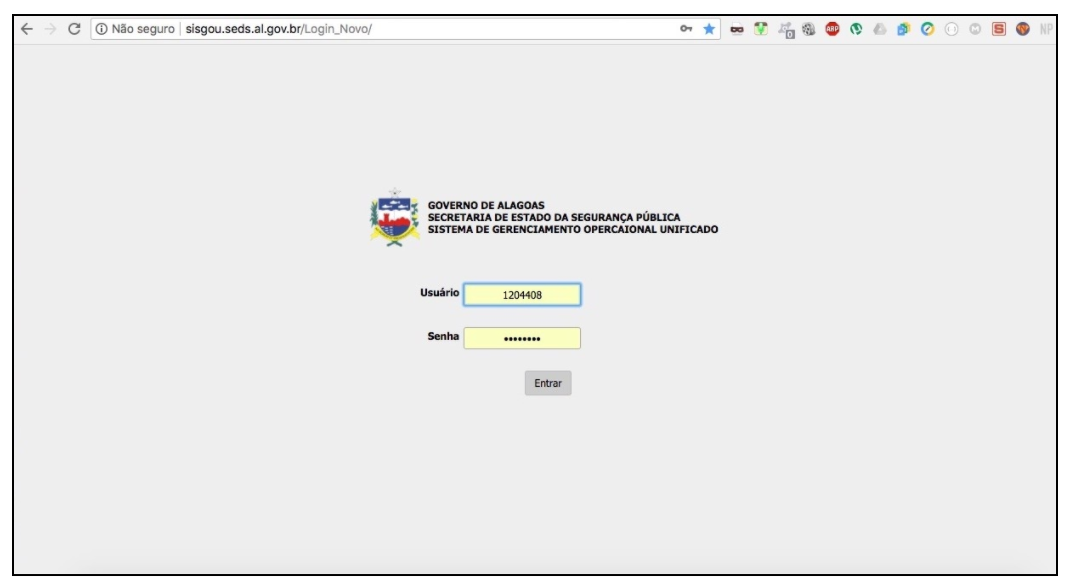
\includegraphics[width=0.6\textwidth]{./04-figuras/figura-13}
    \label{fig:ilustfig13}
\end{figure}
\vspace*{-0,9cm}
{\raggedright \fonte{Dispon\'{i}vel em: <https://https://www.sisgou.seds.al.gov.br>. Acesso em: 13 ago. 2020.}}\\

% FERRAMENTAS

\section{Ferramentas}

% SGDB POSTGRESQL

\subsection{SGDB PostgreSQL}

O PostgreSQL \'{e} um sistema de gerenciamento de banco de dados relacional de objeto (ORDBMS) baseado no 
PostgreSQL, vers\~{a}o 4.2, desenvolvido no Departamento de Ciência da Computa\c{c}\~{a}o da Universidade da Calif\'ornia em \textit{Berkeley}. O PostgreSQL foi pioneiro em muitos conceitos que s\'{o} se tornaram dispon\'{i}veis em alguns sistemas de bancos de dados comerciais muito depois.

Al\'{e}m disso, o PostgreSQL pode ser estendido pelo usu\'{a}rio de v\'{a}rias maneiras, por exemplo, 
adicionando tipos de dados, fun\c{c}\~{o}es, operadores, fun\c{c}\~{o}es agregadas, m\'{e}todos de \'{i}ndice e uma linguagens processuais. Que n\~{a}o ser\~{a}o especificados nesse trabalho.

E por causa da licen\c{c}a liberal, o PostgreSQL pode ser usado, modificado e distribu\'{i}do gratuitamente por 
qualquer pessoa, seja para fins particulares, comerciais ou acadêmicos.

Em nosso trabalho a cria\c{c}\~{a}o, modelagem e o armazenamento dos dados do \textit{Data Warehouse} foi 
utilizado o PostgreSQL, vers\~{a}o 9.5, e com gerenciador administrativo o aplicativo ``pgAdmin'' vers\~{a}o 4. 

Para gerenciar o PostgreSQL, podemos fazê-lo de duas maneiras: uma por meio de uma 
s\'{e}rie de comandos SQL e ou atrav\'{e}s do aplicativo ``pgAdmin''. Neste trabalho enfocaremos o artif\'{i}cio da cria\c{c}\~{a}o do banco de dados, suas tabelas e \textit{constraints}, usando a interface gr\'{a}fica do aplicativo acima, e tamb\'{e}m atrav\'{e}s do PDI, que gera \textit{scripts} com as instru\c{c}\~{o}es para a cria\c{c}\~{a}o da tabela, atrav\'{e}s do processo de transforma\c{c}\~{a}o, criado no PDI, que ser\'{a} mencionado em um t\'opico espec\'{i}fico.

\begin{figure}[H]
	\vspace*{0,2cm}
    \centering
    \caption{Ferramenta ``pgAdmin' vers\~{a}o 4 para o PostgreSQL}
    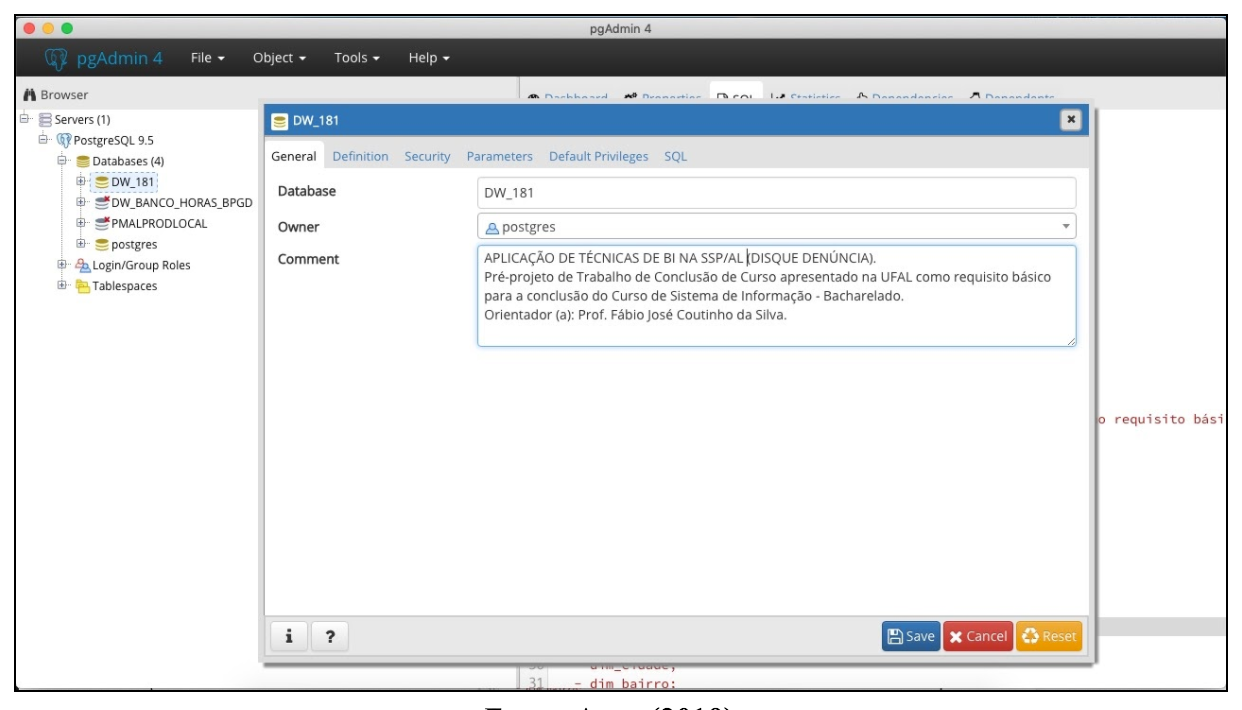
\includegraphics[width=0.6\textwidth]{./04-figuras/figura-14}
    \label{fig:ilustfig14}
\end{figure}
\vspace*{-0,9cm}
{\raggedright \fonte{Autor desta monografia, 2020.}} \\

% PENTAHO

\subsection{Plataforma Pentaho}

Outra ferramenta fundamental neste trabalho \'{e} a Plataforma de Integra\c{c}\~{a}o de Dados e An\'{a}lise Pentaho, nele iremos implementar todos os conceitos de DW/BI. Para isso precisamos conhecer um pouco sobre essa ferramenta, conforme figura abaixo.

\begin{figure}[H]
	\vspace*{0,2cm}
    \centering
    \caption{\textit{Pentaho Business Analytics Platform}}
    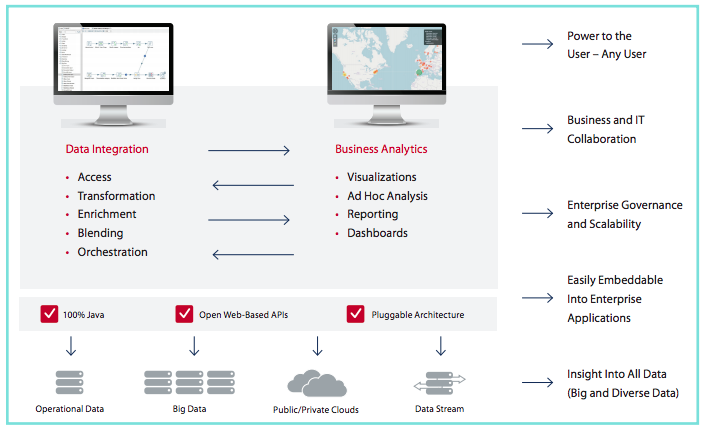
\includegraphics[width=0.6\textwidth]{./04-figuras/figura-15}
    \label{fig:ilustfig15}
\end{figure}
\vspace*{-0,9cm}
{\raggedright \fonte{Dispon\'{i}vel em: <https://https://www.hitachivantara.com/en\_us/pdf/datasheet/pentaho-business-analytics-platform-datasheet.pdf>. Acesso em: 16 ago. 2020.}}\\

Os produtos Pentaho s\~{a}o abrangentes e usados para acessar, integrar, manipular, visualizar e analisar seus dados. 
Quer os dados sejam armazenados em um arquivo simples, banco de dados relacional, \textit{cluster Hadoop}, banco de dados 
NoSQL, banco de dados anal\'{i}tico, fluxos de m\'{i}dia social, lojas operacionais ou na nuvem, os produtos Pentaho 
podem ajud\'{a}-lo a descobrir, analisar e visualizar dados para encontrar as respostas que você precisa, mesmo se 
você n\~{a}o tiver experiência em codifica\c{c}\~{a}o. 
Usu\'{a}rios avan\c{c}ados com experiência em programa\c{c}\~{a}o podem usar nossa ampla API\index{API}\footnote{API: 
Ë um conjunto de rotinas e padr\~{o}es de programa\c{c}\~{a}o para acesso a um aplicativo de software ou plataforma 
baseado na Web. A sigla API refere-se ao termo em inglês ``\textit{Application Programming Interface}'' que 
significa em tradu\c{c}\~{a}o para o português ``Interface de Programa\c{c}\~{a}o de Aplicativos``.} para personalizar 
relat\'orios, consultas e transforma\c{c}\~{o}es para estender a funcionalidade.

Os produtos Pentaho incluem componentes baseados na web e ferramentas de \textit{design}. Os componentes e 
ferramentas que você usa dependem do seu fluxo de trabalho e do que seu ambiente oferece suporte

Toda plataforma est\'{a} dividida em duas partes: Componentes baseados na web e as Ferramentas de \textit{Design}.

Os componentes baseados na web s\~{a}o:

\begin{itemize}
    \item Console de usu\'{a}rio: O \textit{Pentaho User Console} (PUC) \'{e} um ambiente de design para acessar \textit{Analyzer}, Relat\'orios Interativos e \textit{Dashboard Designer}. \textit{Pentaho User Console} tamb\'{e}m oferece recursos de administra\c{c}\~{a}o do sistema para configurar seu servidor Pentaho.
    \item Analisador: O \textit{Analyzer} ajuda a visualizar dados para tomar decis\~{o}es de neg\'ocios informadas. Você pode criar visualiza\c{c}\~{o}es geogr\'{a}ficas, gr\'{a}fico de dispers\~{a}o, grade de calor e múltiplos gr\'{a}ficos. Você tamb\'{e}m pode filtrar dados, adicionar par\^{a}metros de consulta, configurar links de pesquisa detalhada, aplicar formata\c{c}\~{a}o condicional e gerar \textit{hiperlinks}. Em nosso trabalho iremos utilizar dois analisadores: o \textit{Saiku} e o \textit{JPivo}t.
    \item Relat\'orios Interativos: Relat\'orios interativos s\~{a}o uma interface de design usada para criar relat\'orios operacionais simples e sob demanda, sem depender de TI ou desenvolvedores de relat\'orios. Você pode adicionar rapidamente elementos ao seu relat\'orio e format\'{a}-los da maneira que desejar.
    \item \textit{Dashboard Designer}: O \textit{Dashboard Designer} \'{e} usado para escolher modelos de layout, temas e conteúdo para criar pain\'{e}is visualmente atraentes que ajudam os tomadores de decis\~{a}o a obter conhecimento cr\'{i}tico rapidamente. Você pode combinar uma ampla variedade de conteúdo, incluindo relat\'orios interativos, visualiza\c{c}\~{o}es do \textit{Analyzer} e conteúdo colaborativo.
    \item CTools: CTools \'{e} uma estrutura orientada pela comunidade para a cria\c{c}\~{a}o de pain\'{e}is usando tecnologias da web, como \textit{JavaScript}, CSS e HTML. Você pode criar facilmente pain\'{e}is din\^{a}micos para os usu\'{a}rios explorarem e entenderem grandes quantidades de dados usando uma variedade de gr\'{a}ficos, tabelas e outros componentes.
    \item Assistente de fonte de dados: O \textit{Data Source Wizard} ajuda a definir uma fonte de dados que cont\'{e}m suas informa\c{c}\~{o}es e o orienta na cria\c{c}\~{a}o de seus primeiros modelos relacionais ou multidimensionais para uso na cria\c{c}\~{a}o de relat\'orios e an\'{a}lises.
    \item Editor de modelo de fonte de dados: O Editor de modelo de fonte de dados ajuda a ajustar e refinar modelos de dados relacionais e multidimensionais. Você pode arrastar campos para seus locais apropriados, misturar e combinar campos de diferentes tabelas, adicionar campos a mais de uma categoria ou remover um campo.
\end{itemize}

As ferramentas de design da Pentaho s\~{a}o usadas para desenvolver e refinar como os valores dos dados s\~{a}o relatados, modelados, transformados e armazenados. Elas s\~{a}o:

\begin{itemize}
    \item Integra\c{c}\~{a}o de dados: \textit{Pentaho Data Integration} (PDI) fornece acesso a um motor de Extra\c{c}\~{a}o, Transforma\c{c}\~{a}o e Carregamento (ETL) que captura os dados certos, limpa os dados e armazena os dados usando um formato uniforme que \'{e} acess\'{i}vel e relevante para os usu\'{a}rios finais e tecnologias IoT\index{NewR}\footnote{IoT: \textit{Internet Of Tink} ou Internet das coisas \'{e} um conceito que se refere \`{a} interconex\~{a}o digital de objetos cotidianos com a internet, conex\~{a}o dos objetos mais do que das pessoas. Em outras palavras, a internet das coisas nada mais \'{e} que uma rede de objetos f\'{i}sicos capaz de reunir e de transmitir dados.}
    \item \textit{Report Designer}: O \textit{Report Designer} \'{e} usado para gerar relat\'orios detalhados e perfeitos em pixels, usando virtualmente qualquer fonte de dados. Ele permite que os profissionais de \textit{business intelligence} criem relat\'orios altamente detalhados e com qualidade de impress\~{a}o, com base em dados preparados de maneira adequada.
    \item Designer de agrega\c{c}\~{a}o: O \textit{Aggregation Designer} fornece uma interface simples que permite criar tabelas agregadas de n\'{i}veis dentro das dimens\~{o}es que você especificar. Use esta ferramenta para melhorar o desempenho de seus cubos OLAP \textit{Pentaho Analysis} (Mondrian).
    \item Editor de Metadados: O Editor de Metadados simplifica a constru\c{c}\~{a}o de relat\'orios. Use o Editor de Metadados para construir dom\'{i}nios e modelos de metadados Pentaho. Um \textit{Pentaho Metadata Model} mapeia a estrutura f\'{i}sica do seu banco de dados em um modelo de neg\'ocio l\'ogico.
    \item \textit{Schema Workbench}: \textit{Schema Workbench} permite editar e criar modelos multidimensionais (Mondrian). Você pode criar modelos Mondrian graficamente ou defini-los codificando manualmente os arquivos XML.
\end{itemize}

Nesta plataforma est\~{a}o dispon\'{i}veis componentes para execu\c{c}\~{a}o de processos de ETL, que fazem 
carga de \textit{Data Warehouses}, cria\c{c}\~{a}o de relat\'orios pr\'{e}-formatados e ad hoc, cubos OLAP, 
pain\'{e}is de instrumentos (\textit{Dashboards}) e garimpagem de dados (\textit{Data Mining}). 

Todos esses recursos podem ser combinados e acionados sequencialmente para cria\c{c}\~{a}o de solu\c{c}\~{o}es 
mais sofisticadas. Al\'{e}m disso, a plataforma executa todas as solu\c{c}\~{o}es de BI como servi\c{c}os e, 
por isso, \'{e} poss\'{i}vel prover acesso \`{a}s solu\c{c}\~{o}es para sistemas externos, via 
\textit{web services}, atrav\'{e}s de um mecanismo baseado em SOAP/WSDL/UDDI.

Por\'{e}m, n\~{a}o iremos neste trabalho nos deter em todos estes recurso, apenas o m\'{i}nimo para 
uma solu\c{c}\~{a}o vi\'{a}vel para o servi\c{c}o do 181.

% DESENVOLVENDO A SOLU\c{c}\~{a}O

\section{Desenvolvimento da Solu\c{c}\~{a}o}

Com base nos conceitos do capitulo de Fundamenta\c{c}\~{a}o, e as t\'{e}cnicas de Kimball(2013), 
iremos aplicar estes conhecimentos na implementa\c{c}\~{a}o de um BI/DW, que ser\'{a} desenvolvido 
sobre um servidor local, usando todo o potencial e simplicidade da Plataforma Pentaho, desde o download 
do arquivo no formato ``.XLS``, com os dados de denúncias consultadas na aplica\c{c}\~{a}o web SISGOU, ao 
processamento ETL usando o PDI do Pentaho, e o OLAP usando o \textit{Saiku Analytics} e at\'{e} o 
\textit{dashboard} (painel) usando o CTOOLS e a cria\c{c}\~{a}o de um relat\'orio com o PRD.

% Banco de dados
\subsection{Criando nosso Banco de dados}

O nosso trabalho ir\'{a} precisar de um Banco de dados no SGBD PostgreSQL, que podemos 
criar via terminal do macOSX, por\'{e}m, usamos o aplicativo ``pgAdmin4''
que gerencia todos o banco de dados visualmente, economizando tempo de digita\c{c}\~{a}o, conforme figura abaixo.

\begin{figure}[H]
	\vspace*{0,2cm}
    \centering
    \caption{\textit{Script} do Banco de dados da solu\c{c}\~{a}o}
    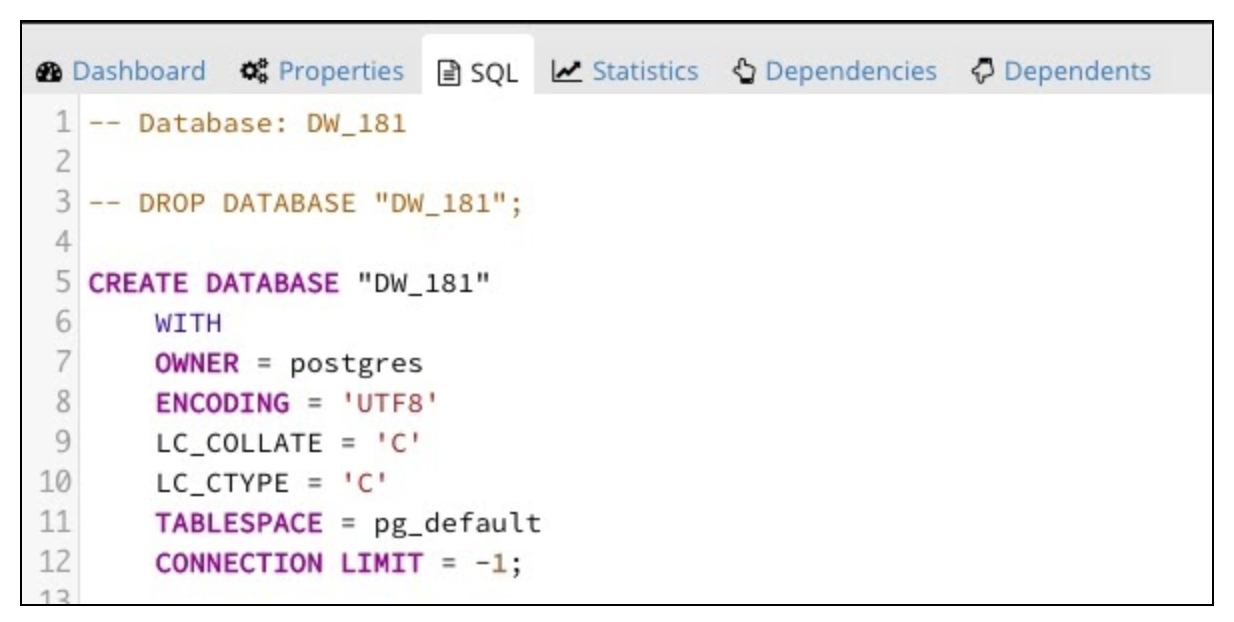
\includegraphics[width=0.6\textwidth]{./04-figuras/figura-16}
    \label{fig:ilustfig16}
\end{figure}
\vspace*{-0,9cm}
{\raggedright \fonte{Autor desta monografia, 2020.}} \\

Acessando o ``pdAmin4'', e digitando esse comando da figura acima e basta apenas executar o mesmo na ferramenta 
que o Banco de dados ser\'{a} criando. Iniciando assim o primeiro passado para criarmos nossa ETL.

\subsection{Criando o processo de ETL}

Ap\'os termos dado o primeiro passo, teremos como base do processo de Extra\c{c}\~{a}o o arquivo no 
formato do \textit{Microsoft Excel} denominado ``181.xls'', lembrando que o mesmo foi exportado ``do 
Aplicativo Web SISGOU'' na op\c{c}\~{a}o de consulta. 

Ele ter\'{a} o mesmo formado da figura abaixo, como suas 
linhas e colunas totalmente sem normatiza\c{c}\~{a}o aparente e sem nenhum tratamento nos dados.

% FALTA A figura
\begin{figure}[H]
	\vspace*{0,2cm}
    \centering
    \caption{Arquivo extra\'{i}do da consulta do Disque denúncia do  SISGOU}
    
\includegraphics[width=0.6\textwidth]{./04-figuras/falta-figura.png}
    \label{fig:ilustfigfaltafigura01}
\end{figure}
\vspace*{-0,9cm}
{\raggedright \fonte{Autor desta monografia, 2020.}} \\

Para criarmos nosso processo de ETL no arquivo acima, precisamos usar o \textit{Pentaho Data Integration}, para isso precisamos instalar o mesmo junto com toda Plataforma Pentaho. E ap\'os instalado,  clicaremos com o mouse no \'{i}cone do \textit{Data Integration}, a tela de boas vindas do PDI aparece, de acordo com a figura abaixo e depois surge a interface da aplica\c{c}\~{a}o que ser\'{a} usada para a configura\c{c}\~{a}o dos processo de ETL, que transformar\~{a}o os dados em \textit{Microsoft Excel} com dados formatado por um SGBD relacional.

\begin{figure}[H]
	\vspace*{0,2cm}
    \centering
    \caption{tela de Boas Vinda e a Interface do PDI (\textit{Pentaho Data Integration}).}
    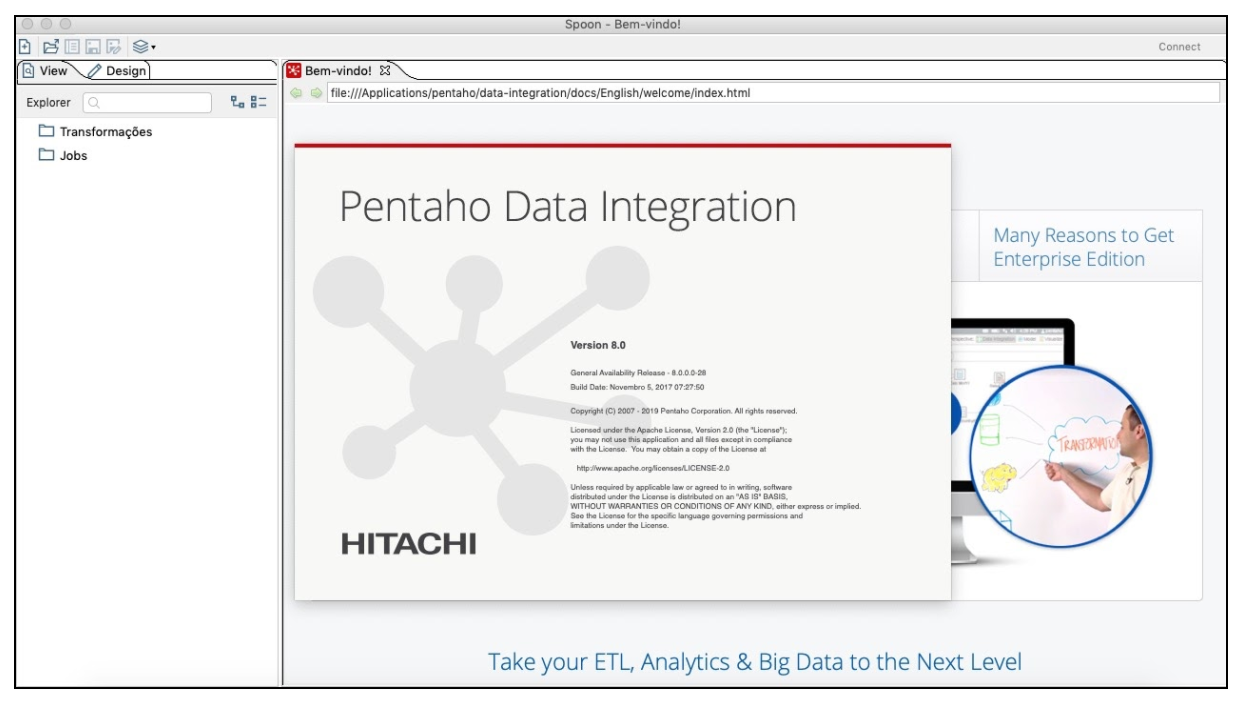
\includegraphics[width=0.6\textwidth]{./04-figuras/figura-pentaho-pdi}
    \label{fig:ilustfigpentaho-pdi}
\end{figure}
\vspace*{-0,9cm}
{\raggedright \fonte{Autor desta monografia, 2020.}} \\

O \textit{Pentaho Data Integration}, fornece os recursos \textit{Extract, Transform e Load} (ETL) que facilitam o processo de captura, limpeza e armazenamento de dados usando um formato uniforme e consistente que \'{e} acess\'{i}vel e relevante para os usu\'{a}rios finais e tecnologias IoT.

O PDI \'{e} formado por duas categorias de artefatos, \textit{Jobs} e Transforma\c{c}\~{o}es, e estes artefatos s\~{a}o constru\'{i}dos por meio de sua interface gr\'{a}fica, o \textit{Spoon}. 

O \textit{Spoon} \'{e} a interface gr\'{a}fica do \textit{Pentaho Data Integration} que facilita na concep\c{c}\~{a}o de rotinas e l\'ogica ETL. Abaixo na figura apresentamos a interface do PDI.

\begin{figure}[H]
	\vspace*{0,2cm}
    \centering
    \caption{Spoon do PDI (\textit{Pentaho Data Integration}).}
    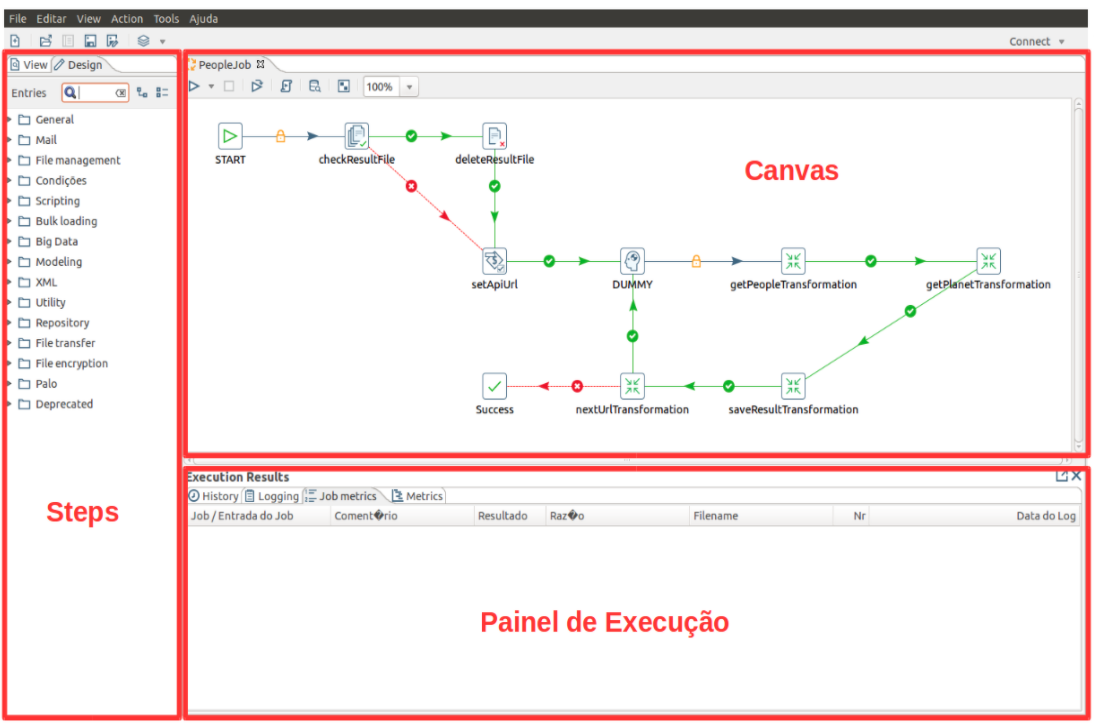
\includegraphics[width=0.6\textwidth]{./04-figuras/figura-pentaho-pdi-spoon}
    \label{fig:ilustfigpentaho-pdi-spoon}
\end{figure}
\vspace*{-0,9cm}
{\raggedright \fonte{Autor desta monografia, 2020.}} \\

Que ser\~{a}o nomeadas no banco de dados ``DW\_181'' como: dim\_bairro, dim\_cidade, dim\_origem, dim\_tipo-denncia, dim\_data, dim\_hora e o fato\_denuncia.

Quando todas as transforma\c{c}\~{o}es das dimens\~{o}es e do fato forem desenvolvidas iremos un\'{i}-las em um processo denominado \textit{Job}, que agregar\'{a} todas as transforma\c{c}\~{o}es para uma execu\c{c}\~{a}o única de toda ETL.

O primeiro passo \'{e} criar a conex\~{a}o usando o componente \textit{Database Connection}, em nosso trabalho usaremos o nome ``CNN\_DW\_181'' para a conex\~{a}o com o banco de dados local ``DW\_181'', na porta de número: ``5432'', usu\'{a}rio: ``postgres'', conforme figura abaixo.

\begin{figure}[H]
	\vspace*{0,2cm}
    \centering
    \caption{\textit{Database Connection - ``CNN\_DW\_181''}}
    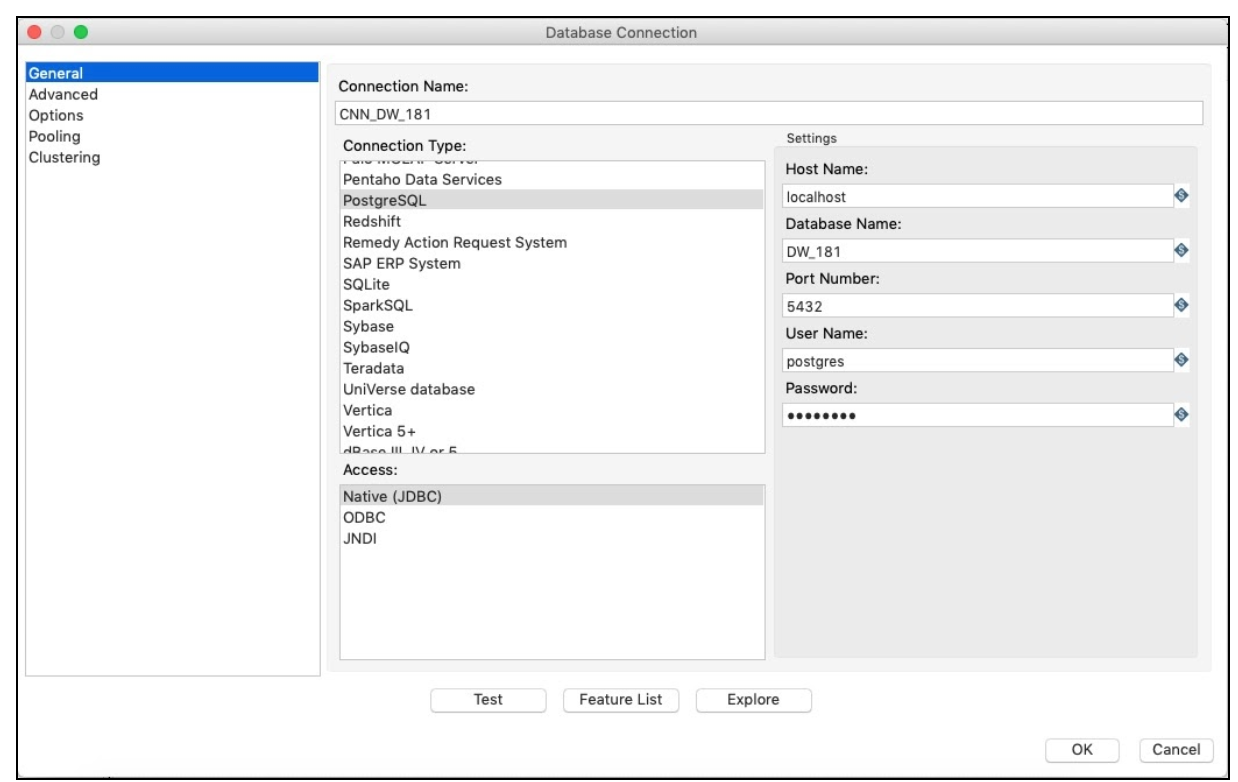
\includegraphics[width=0.6\textwidth]{./04-figuras/figura-pentaho-database-connection}
    \label{fig:ilustfigpentaho-database-connection}
\end{figure}
\vspace*{-0,9cm}
{\raggedright \fonte{Autor desta monografia, 2020.}} \\

% TRANSFORMA\c{c}\~{o}ES
\subsubsection{Criando as transforma\c{c}\~{o}es no PDI}

Ap\'os a termos criado no t\'opico anterior a conex\~{a}o ``CNN\_DW\_181'', iniciaremos a desenvolvimento das transforma\c{c}\~{o}es. Para isso se faz necess\'{a}rio o uso de alguns \textit{steps}. que iniciam do do acesso aos dados no arquivo com os dados a serem transformado at\'{e} a cria\c{c}\~{a}o e carga da dimens\~{a}o que far\~{a}o parte do modelo Dimensional Estrela j\'{a} definido neste trabalho.

Para criarmos as transforma\c{c}\~{o}es que ao final sejam geradas \`{a}s dimens\~{o}es, precisamos usar a aba \textit{Design} e os componentes nela presentes.

Para melhorar o entendimento padronizamos um nomenclatura para os arquivos das transforma\c{c}\~{o}es, formato ``.ktr'', e do \textit{Job}\index{job}\footnote{\textit{Job}: \'{e} o processo que une todas \`{a}s transforma\c{c}\~{o}es para uma execu\c{c}\~{a}o de todas dentro do PDI}, formato ``.kjb'', para ajudar no desenvolvimento do DW/BI. Para transforma\c{c}\~{o}es de dimens\~{o}es: ``dim\_nome da dimens\~{a}o.ktr'' e para o fato: ``fato\_nome do fato.ktr
''.

Na constru\c{c}\~{a}o das nossas transforma\c{c}\~{o}es e nesta fase de ETL como um todo utilizaremos o componente de step: \textit{Microsoft Excel Input}, figura abaixo, que est\'{a} localizado na barra lateral de Design do \textit{Spoon}, na categoria \textit{input}. Este componente em especial ser\'{a} o padr\~{a}o para o acesso aos dados da planilha em no formato do \textit{Microsoft Excel}, e nome ``181.xls'' em todas as transforma\c{c}\~{o}es.

O \textit{step Microsoft Excel Input} tem como principais fun\c{c}\~{o}es dar acesso ao dados e fazer ajustes nos nomes, tipos e tamanhos das colunas.

\begin{figure}[H]
	\vspace*{0,2cm}
    \centering
    \caption{Barra lateral do PDI e o Componente \textit{step Microsoft Excel Input}}
    
\includegraphics[width=0.6\textwidth]{./04-figuras/falta-figura.png}
    \label{fig:ilustfigfaltafigura02}
\end{figure}
\vspace*{-0,9cm}
{\raggedright \fonte{Autor desta monografia, 2020.}} \\

Quando acessamos o \textit{step Microsoft Excel Input} temos acesso a tela conforme da figura abaixo, nela temos as abas \textit{Files, Sheets, Content, Error Handing, Fields e Additional output fields}. Por\'{e}m, vamos apenas nos focar na aba \textit{Fields} que cont\'{e}m os campos providos da fonte de dados. 

Nela podemos fazer os ajustes necess\'{a}rios para que a transforma\c{c}\~{a}o ao longo dos \textit{steps Select values, Sort rows, Unique rows, Value Mapper, Add sequence, Table output} recebam os dados n\~{a}o transformados que ser\~{a}o ao longo dos \textit{steps} ajustados para que ao final tenhamos a dimens\~{a}o pretendida com os dados padronizados .

\begin{figure}[H]
	\vspace*{0,2cm}
    \centering
    \caption{Componente \textit{step Microsoft Excel Input}}
    
\includegraphics[width=0.6\textwidth]{./04-figuras/falta-figura.png}
    \label{fig:ilustfigfaltafigura03}
\end{figure}
\vspace*{-0,9cm}
{\raggedright \fonte{Autor desta monografia, 2020.}} \\

% Transforma\c{c}\~{o}es

% dim\_bairros.ktr
\subsubsection{Criando a transforma\c{c}\~{a}o ``dim\_bairro.ktr''}

Os componentes que far\~{a}o parte da transforma\c{c}\~{a}o ``dim\_bairro.ktr'', ser\~{a}o: \textit{Microsoft Excel Input, Select values, Sort rows, Unique rows, Value Mapper, Add sequence} e finalmente \textit{Table Table output} conforme figura abaixo.

\begin{figure}[H]
	\vspace*{0,2cm}
    \centering
    \caption{Componente \textit{step Microsoft Excel Input.}}
    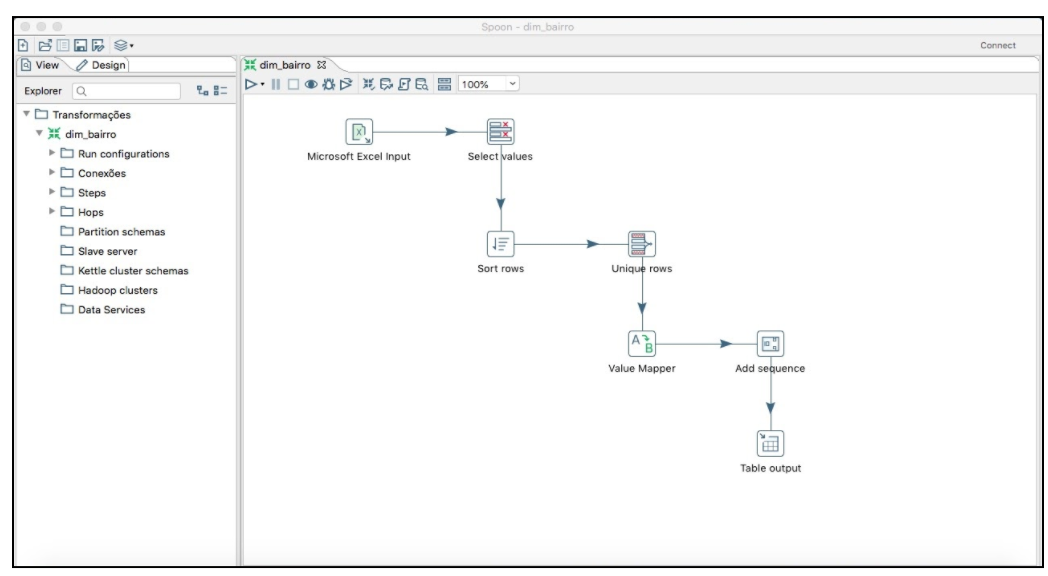
\includegraphics[width=0.6\textwidth]{./04-figuras/figura-dim-bairro}
    \label{fig:ilustfigdimbairro}
\end{figure}
\vspace*{-0,9cm}
{\raggedright \fonte{Autor desta monografia, 2020.}} \\

Primeiramente iremos configurar o \textit{step Select Value} (Selecione o Valor), e na aba \textit{Select and Alter}, na op\c{c}\~{a}o \textit{Fields, Rename to}, iremos modificar o nome Bairro para ``ds\_bairro'', nesse componente ser\'{a} apenas essa a altera\c{c}\~{a}o, conforme figura do quadro tela do \textit{step Select Value}.

Ap\'os  componente \textit{Select Value}, iremos configurar o \textit{step Sort rows} (Organizar a linha), na op\c{c}\~{a}o \textit{Fields}, \textit{Ascending} como ``S'', para que os dados fiquem organizado de forma ascendente, figura do quadro tela do \textit{step Sort rows}.

O pr\'oximo componente \'{e} \textit{Unique rows} que tem a caracter\'{i}stica de selecionar apenas os valores únicos das linhas, ou seja, evitar a duplica\c{c}\~{a}o, nesse componente h\'{a} apenas a necessidade de configurar o nome do campo ou \textit{Fieldname}, conforme a figura da tela do \textit{step Unique rows}.

O componente \textit{Value Mapper}, em s\'{i}ntese tem como fun\c{c}\~{a}o trocar os valores vindos da linha da fonte de dados que ser\~{a}o comparados no \textit{Source Value}, e ap\'os encontrar o mesmo ela ser\'{a} trocado pelo informado em \textit{Target value}, conforme a figura da tela do \textit{step Value Mapper}.

Ap\'os transformarmos os dados brutos da linha Bairro da fonte de dado em Ms \textit{Microsoft Excel}, iremos criar um campo sequencial, para isso usaremos o componente \textit{Add sequence}, a única altera\c{c}\~{a}o ser\'{a} no op\c{c}\~{a}o Nome do valor, que foi mudado para ``id\_bairro'', conforme figura da tela do \textit{Add sequence}.

Finalizando a transforma\c{c}\~{a}o ``dim\_bairro.ktr'', usaremos o componente \textit{Table output} nele iremos alterar as op\c{c}\~{o}es \textit{Connection, Target schema, Target table, truncate table}, e na aba \textit{Database fields}, incluiremos os Campos ou colunas da tabela ``dim\_bairro'' que ser\'{a} criada ap\'os finalizar essa etapa de configura\c{c}\~{a}o dos componentes da transforma\c{c}\~{a}o, conforme \`{a} figura da tela do \textit{step Table output}.

\begin{figure}[H]
	\vspace*{0,2cm}
    \centering
    \caption{Configurando os \textit{steps} da Transforma\c{c}\~{a}o ``dim\_bairros.ktr''(passo-a-passo).}
    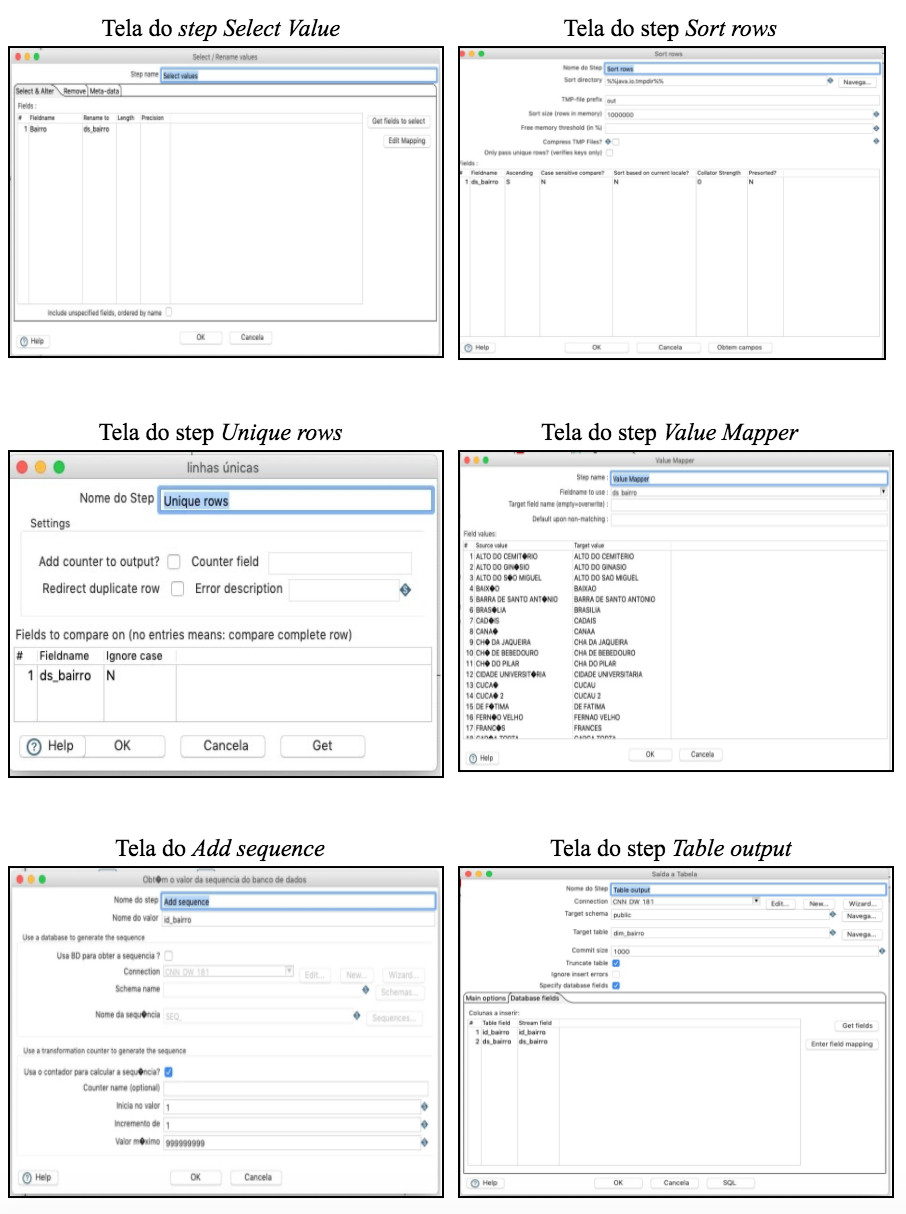
\includegraphics[width=0.6\textwidth]{./04-figuras/figura-passos-dim-bairros}
    \label{fig:ilustfigpassasdimbairros}
\end{figure}
\vspace*{-0,9cm}
{\raggedright \fonte{Autor desta monografia, 2020.}} \\

Ap\'os ter ajustado a configura\c{c}\~{a}o do \textit{step Table output}, selecionaremos o bot\~{a}o SQL, e aparecer\'{a} a tela da figura abaixo, tela \textit{Simple SQL editor}. Na tela do \textit{Simple SQL editor} , selecionando o bot\~{a}o \textit{Execute}, e surgir\'{a} a tela \textit{Results of the SQL statements}, conforme figura abaixo, abaixo. E finalmente criamos o tabela ``dim\_bairro'', dentro do banco de dados 
``DW\_181''.

\begin{figure}[H]
	\vspace*{0,2cm}
    \centering
    \caption{Criando a tabela ``dim\_bairro'' no banco de dados usando o \textit{step Table output}}
    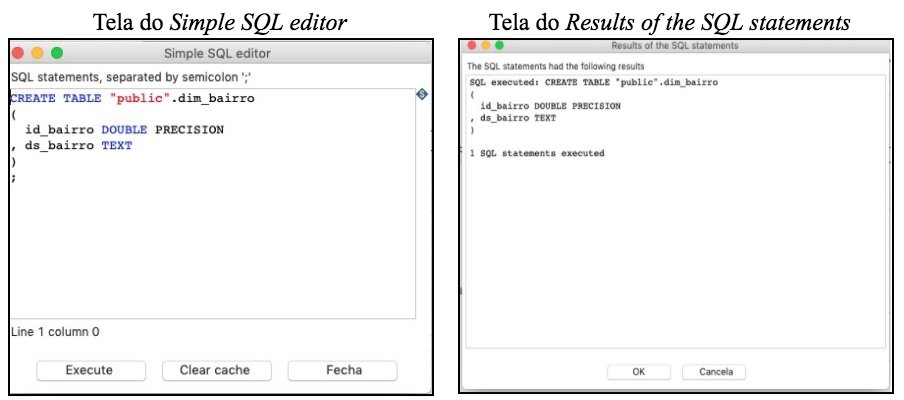
\includegraphics[width=0.6\textwidth]{./04-figuras/figura-tb-dim-bairro}
    \label{fig:ilustfigtbdimbairros}
\end{figure}
\vspace*{-0,9cm}
{\raggedright \fonte{Autor desta monografia, 2020.}} \\

% dim\_cidade.ktr
\subsubsection{Criando a transforma\c{c}\~{a}o ``dim\_cidade.ktr''}

Os componentes que far\~{a}o parte da transforma\c{c}\~{a}o ``dim\_cidade.ktr'', ser\~{a}o: \textit{Microsoft Excel Input, Select values, Sort rows, Unique rows, Value Mapper, Add sequence} e finalmente \textit{Table Table output} conforme figura sabaixo. 

\begin{figure}[H]
	\vspace*{0,2cm}
    \centering
    \caption{Transforma\c{c}\~{a}o ``dim\_cidade.ktr''}
    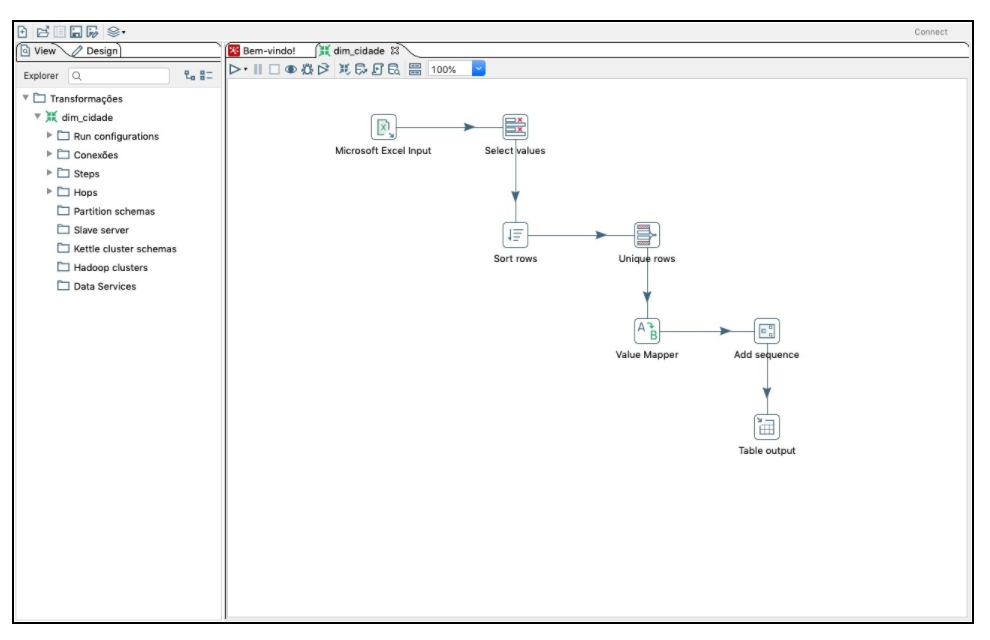
\includegraphics[width=0.6\textwidth]{./04-figuras/figura-trans-dim-cidade}
    \label{fig:ilustfigtransdimcidade}
\end{figure}
\vspace*{-0,9cm}
{\raggedright \fonte{Autor desta monografia, 2020.}} \\

Primeiramente iremos configurar o \textit{step Select Value} (Selecione o Valor), e na aba \textit{Select and Alter}, na op\c{c}\~{a}o \textit{Fields, Rename to}, teremos que modificar o nome Bairro para ``ds\-bairro'', nesse componente ser\'{a} apenas essa a altera\c{c}\~{a}o, conforme figura do quadro tela do \textit{step Select Value}.

Ap\'os  componente \textit{Select Value}, iremos configurar o \textit{step Sort rows} (Organizar a linha), na op\c{c}\~{a}o \textit{Fields, Ascending} como ``S'', para que os dados fiquem organizado de forma ascendente, figura do quadro tela do \textit{step Sort rows}.

O pr\'oximo componente \'{e} \textit{Unique rows} que tem a caracter\'{i}stica de selecionar apenas os valores únicos das linhas, ou seja, evitar a duplica\c{c}\~{a}o, nesse componente h\'{a} apenas a necessidade de configurar o nome do campo ou \textit{Fieldname}, conforme a figura da tela do \textit{step Unique rows}.

O componente \textit{Value Mapper}, em s\'{i}ntese tem como fun\c{c}\~{a}o trocar os valores vindos da linha da fonte de dados que ser\~{a}o comparados no \textit{Source Value}, e ap\'os encontrar o mesmo ela ser\'{a} trocado pelo informado em \textit{Target value}, conforme a figura do quadro tela do \textit{step Value Mapper}.

Ap\'os transformarmos os dados brutos da linha ``Cidade'' da fonte de dado em \textit{Microsoft Excel}, iremos criar um campo sequencial, para isso usaremos o componente \textit{Add sequence}, a única altera\c{c}\~{a}o ser\'{a} no op\c{c}\~{a}o Nome do valor, que foi mudado para ``id\_cidade'', conforme figura da tela do \textit{Add sequence}.

Finalizando a transforma\c{c}\~{a}o ``dim\_cidade.ktr'', usaremos o componente Table output nele iremos alterar as op\c{c}\~{o}es \textit{Connection, Target schema, Target table, truncate table}, e na aba \textit{Database fields}, incluiremos os Campos ou colunas da tabela ``dim\_cidade'' que ser\'{a} criada ap\'os finalizar essa etapa de configura\c{c}\~{a}o dos componentes da transforma\c{c}\~{a}o, conforme a figura da tela do \textit{step Table output}.

\begin{figure}[H]
	\vspace*{0,2cm}
    \centering
    \caption{Configurando os \textit{steps} da Transforma\c{c}\~{a}o ``dim\_cidade.ktr'' (passo-a-passo)}
    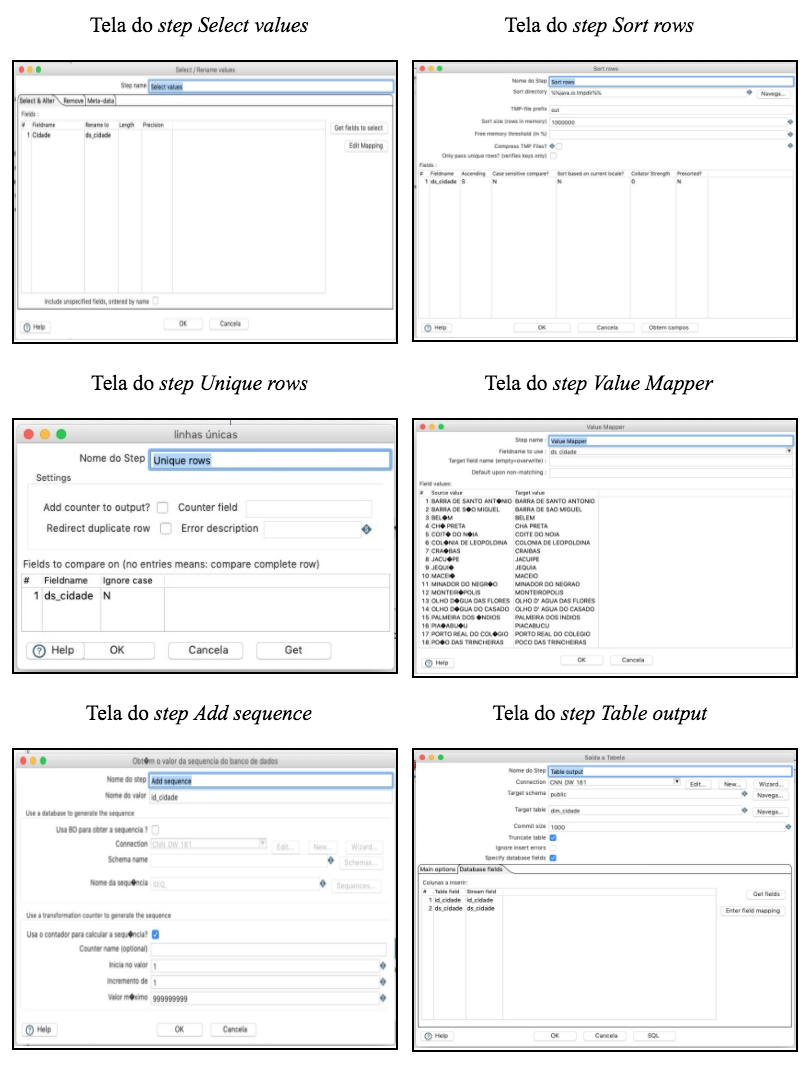
\includegraphics[width=0.6\textwidth]{./04-figuras/figura-dim-cidade-passo-a-passo}
    \label{fig:ilustfigstepdimcidade}
\end{figure}
\vspace*{-0,9cm}
{\raggedright \fonte{Autor desta monografia, 2020.}} \\

\begin{figure}[H]
	\vspace*{0,2cm}
    \centering
    \caption{Criando a tabela ``dim\_cidade'' no banco de dados usando o \textit{step Table output}}
    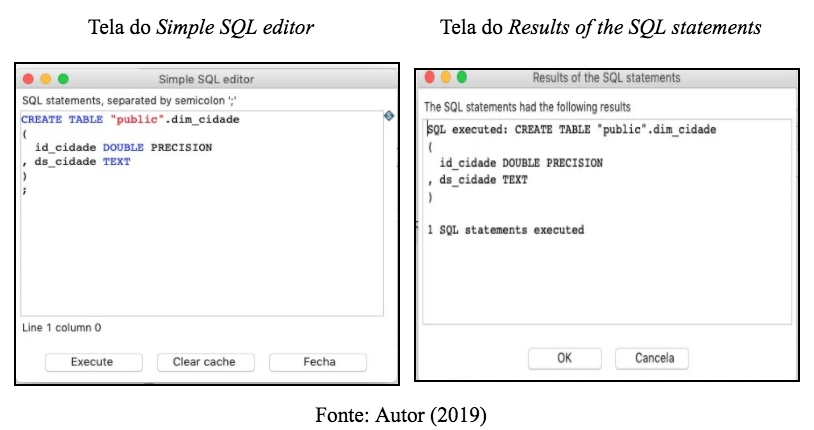
\includegraphics[width=0.6\textwidth]{./04-figuras/figura-tb-dim-cidade}
    \label{fig:ilustfigtbdimcidade}
\end{figure}
\vspace*{-0,9cm}
{\raggedright \fonte{Autor desta monografia, 2020.}} \\

Ao final dos processos quando executamos a transforma\c{c}\~{a}o, conforme figura abaixo, na parte posterior da tela do PDI, em ``Execution Results''. aparecer\'{a} na aba ``Preview data'', os dados padronizados dos campos: ``ds\_cidade'' e ``id\_cidade''. O pr\'oximo passo ser\'{a} percorrer a grade com os resultado e perceber se o processo de transforma\c{c}\~{a}o e carga sai conforme planejado. 

\begin{figure}[H]
	\vspace*{0,2cm}
    \centering
    \caption{Executando a transforma\c{c}\~{a}o ``dim\_cidade.ktr'' (passo-a-passo)}
    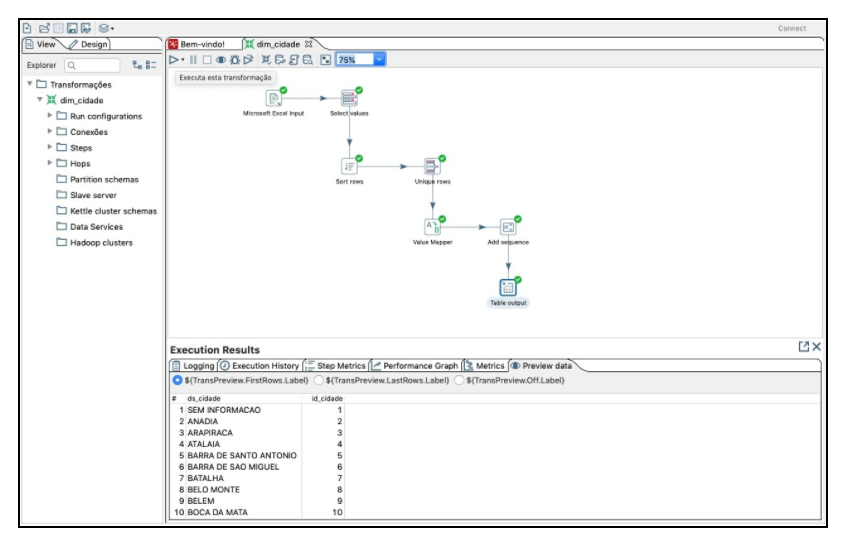
\includegraphics[width=0.6\textwidth]{./04-figuras/figura-exec-dim-cidade}
    \label{fig:ilustfigexecdimcidade}
\end{figure}
\vspace*{-0,9cm}
{\raggedright \fonte{Autor desta monografia, 2020.}} \\

Para termos a certeza de que a tabela ``dim\_cidade'', obteve a ETL correta, precisamos abrir a tabela ``dim\_cidade'' no aplicativo ``pgAdmin 4'', que \'{e} instalado junto ao PostgreSQL, conforme figura abaixo, nela podemos analisar os dados processados pela transforma\c{c}\~{a}o criada no PDI: ``dim\_cidade.ktr''.

\begin{figure}[H]
	\vspace*{0,2cm}
    \centering
    \caption{Resultado da transforma\c{c}\~{a}o e carga no Banco de Dados ``DW\_181'' na tabela ``dim\_cidade''}
    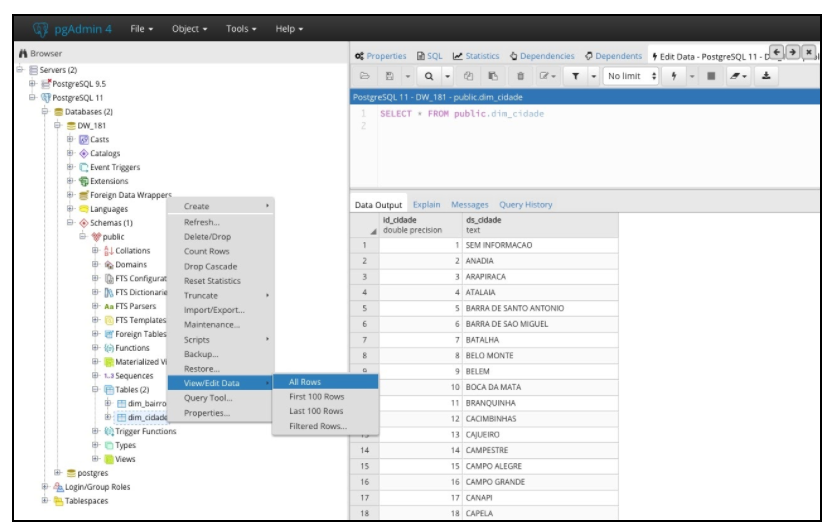
\includegraphics[width=0.6\textwidth]{./04-figuras/figura-res-dim-cidade}
    \label{fig:ilustfigresultdimcidade}
\end{figure}
\vspace*{-0,9cm}
{\raggedright \fonte{Autor desta monografia, 2020.}} \\

% dim\_tipo\_denuncia.ktr
\subsubsection{Criando a transforma\c{c}\~{a}o ``dim\_tipo-denuncia.ktr''}

Os componentes que far\~{a}o parte da transforma\c{c}\~{a}o ``dim\_tipo\_denuncia.ktr'', ser\~{a}o: \textit{Microsoft Excel Input, Select values, Sort rows, Unique rows, Value Mapper, Add sequence} e finalmente \textit{Table Table output} conforme figura abaixo. 

\begin{figure}[H]
	\vspace*{0,2cm}
    \centering
    \caption{Transforma\c{c}\~{a}o ``dim\_tipo\_denuncia.ktr'' do BI do 181.}
    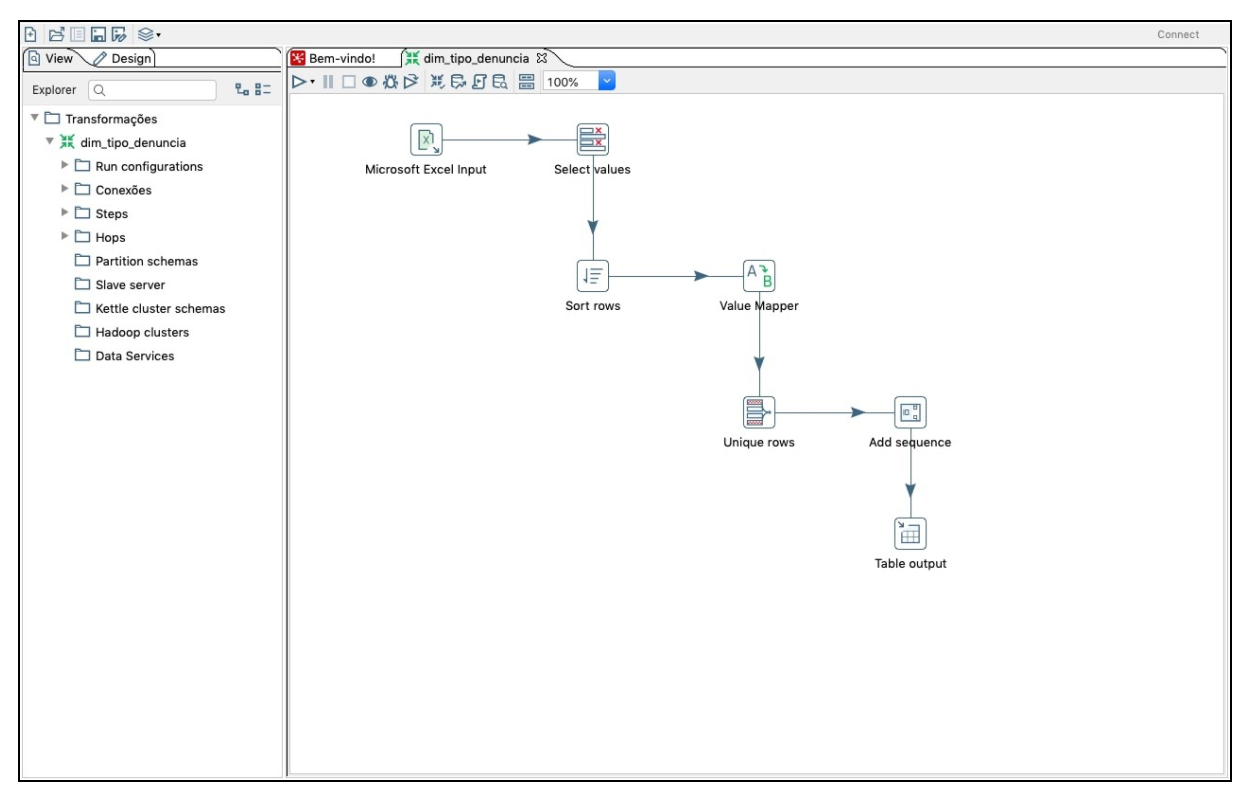
\includegraphics[width=0.6\textwidth]{./04-figuras/figura-dim-tipo-denuncia}
    \label{fig:ilustfigrdimtipodenuncia}
\end{figure}
\vspace*{-0,9cm}
{\raggedright \fonte{Autor desta monografia, 2020.}} \\

Primeiramente iremos configurar o \textit{step Select Value} (Selecione o Valor), e na aba \textit{Select and Alter}, na op\c{c}\~{a}o \textit{Fields, Rename to}, iremos modificar o nome Bairro para ``ds\_tipo\_denuncia'', nesse componente ser\'{a} apenas essa a altera\c{c}\~{a}o, conforme figura da tela da \textit{step Select Value}.

Ap\'os  componente \textit{Select Value}, iremos configurar o \textit{step Sort rows} (Organizar a linha), na op\c{c}\~{a}o \textit{Fields, Ascending} como ``S'', para que os dados fiquem organizado de forma ascendente, figura da tela do \textit{step Sort rows}.

O pr\'oximo componente \'{e} \textit{Unique rows} que tem a caracter\'{i}stica de selecionar apenas os valores únicos das linhas, ou seja, evitar a duplica\c{c}\~{a}o, nesse componente h\'{a} apenas a necessidade de configurar o nome do campo ou \textit{Fieldname}, conforme a figura da tela do \textit{step Unique rows}.

O componente \textit{Value Mapper}, em s\'{i}ntese tem como fun\c{c}\~{a}o trocar os valores vindos da linha da fonte de dados que ser\~{a}o comparados no \textit{Source Value}, e ap\'os encontrar o mesmo ela ser\'{a} trocado pelo informado em \textit{Target value}, conforme a figura da tela do \textit{step Value Mapper}.

Ap\'os transformarmos os dados brutos da linha ``tipo\ denuncia'' da fonte de dado em \textit{Microsoft Excel}, iremos criar um campo sequencial, para isso usaremos o componente \textit{Add sequence}, a única altera\c{c}\~{a}o ser\'{a} no op\c{c}\~{a}o Nome do valor, que foi mudado para ``id\_tipo\_denuncia'', conforme figura da tela do \textit{Add sequence}.

Finalizando a transforma\c{c}\~{a}o ``dim\_tipo\_denuncia.ktr'', usaremos o componente \textit{Table output} nele iremos alterar as op\c{c}\~{o}es \textit{Connection, Target schema, Target table, truncate table}, e na aba \textit{Database fields}, incluiremos os Campos ou colunas da tabela ``dim\_tipo\_denuncia'' que ser\'{a} criada ap\'os finalizar essa etapa de configura\c{c}\~{a}o dos componentes da transforma\c{c}\~{a}o, conforme a figura da tela do \textit{step Table output}.

\begin{figure}[H]
	\vspace*{0,2cm}
    \centering
    \caption{Configurando os \textit{steps} da Transforma\c{c}\~{a}o ``dim\_tipo\_denuncia.ktr'' (passo-a-passo)}
    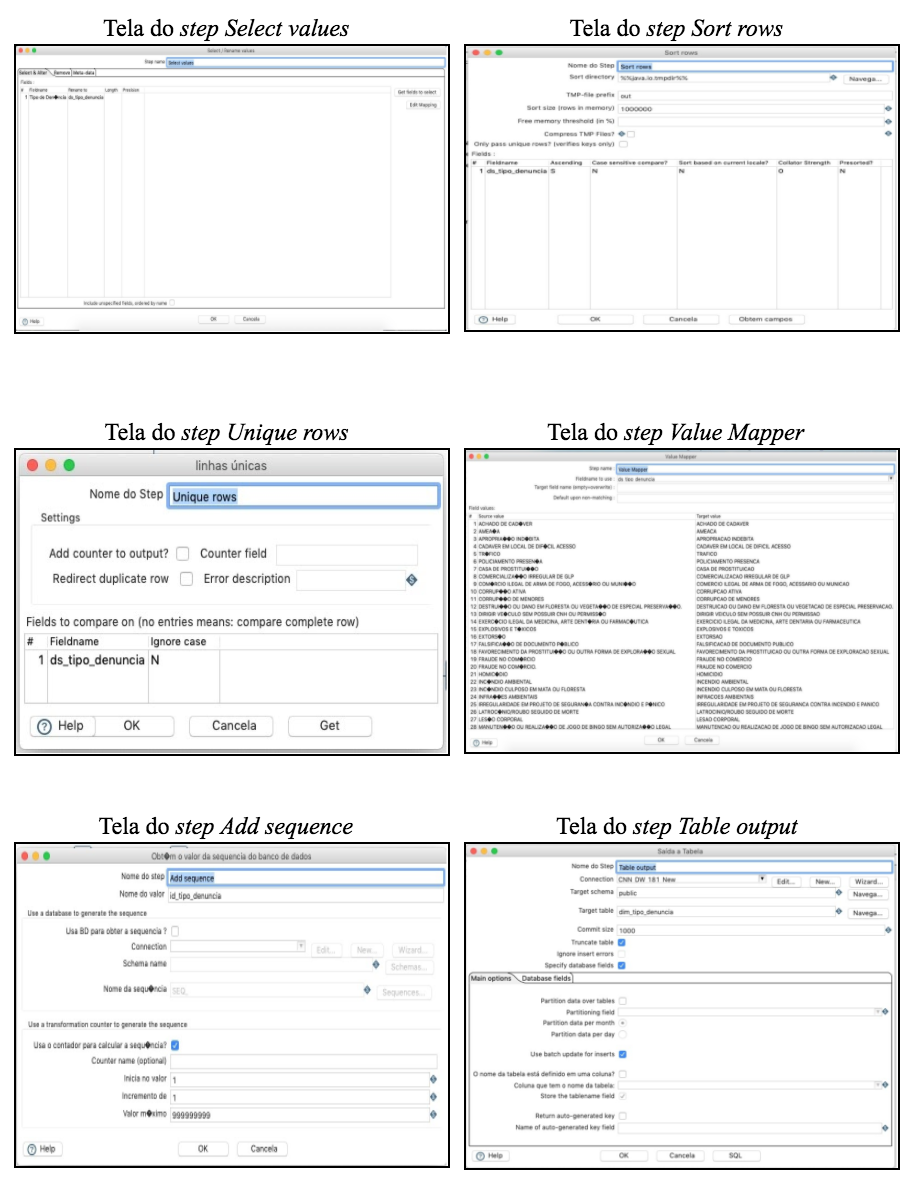
\includegraphics[width=0.6\textwidth]{./04-figuras/figura-dim-tipo-denuncia-passo-a-passo}
    \label{fig:ilustfigrdimtipodenunciapassoapasso}
\end{figure}
\vspace*{-0,9cm}
{\raggedright \fonte{Autor desta monografia, 2020.}} \\

\begin{figure}[H]
	\vspace*{0,2cm}
    \centering
    \caption{Criando a tabela ``dim\_tipo\_denuncia'' no banco de dados usando o \textit{step Table output}}
    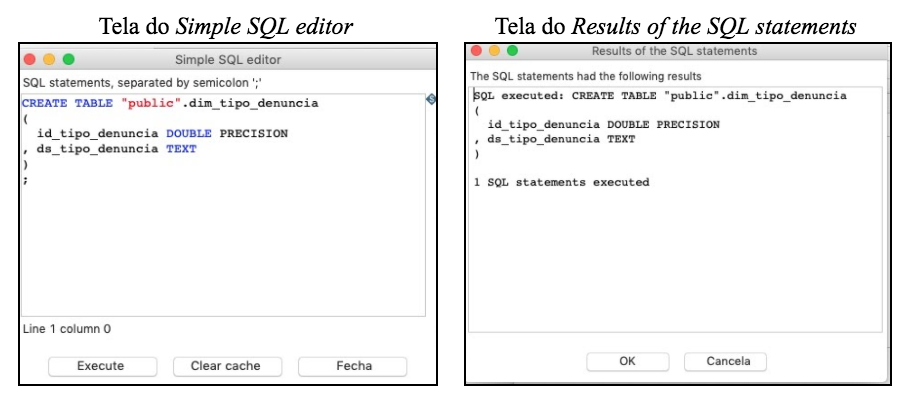
\includegraphics[width=0.6\textwidth]{./04-figuras/figura-tb-dim-tipo-denuncia}
    \label{fig:ilustfigtbdimtipodenuncia}
\end{figure}
\vspace*{-0,9cm}
{\raggedright \fonte{Autor desta monografia, 2020.}} \\

Ao final dos processos quando executamos a transforma\c{c}\~{a}o, conforme figura 48, na parte posterior da tela do PDI, em \textit{Execution Results}. aparecer\'{a} na aba \textit{Preview data}, os dados padronizados dos campos: ``ds\_tipo\_denuncia'' e ``id\_tipo\_denuncia''. O pr\'oximo passo ser\'{a} percorrer a grade com os resultado e perceber se o processo de transforma\c{c}\~{a}o e carga sai conforme planejado. 

\begin{figure}[H]
	\vspace*{0,2cm}
    \centering
    \caption{Executando a transforma\c{c}\~{a}o ``dim\_tipo\_denuncia.ktr''}
    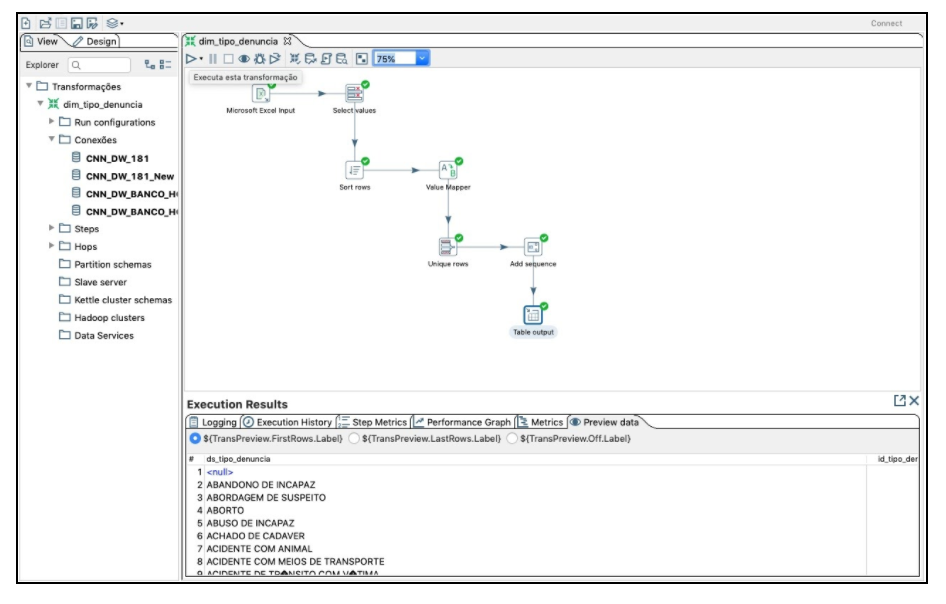
\includegraphics[width=0.6\textwidth]{./04-figuras/figura-trans-tipo-denuncia}
    \label{fig:ilustfigtranstipodenuncia}
\end{figure}
\vspace*{-0,9cm}
{\raggedright \fonte{Autor desta monografia, 2020.}} \\

Para se ter certeza de que a tabela ``dim\_tipo\_denuncia'', obteve a ETL correta, precisamos abrir a tabela ``dim\_tipo\_denuncia'' no aplicativo pgAdmin vers\~{a}o 4, que \'{e} instalado junto ao PostgreSQL, conforme figura 49, nela podemos analisar os dados processados pela transforma\c{c}\~{a}o criada no PDI: ``dim\_tipo\_denuncia.ktr''.

\begin{figure}[H]
	\vspace*{0,2cm}
    \centering
    \caption{Resultado da transforma\c{c}\~{a}o e carga no Banco de Dados ``DW\_181'' na tabela ``dim\_tipo\_denuncia''}
    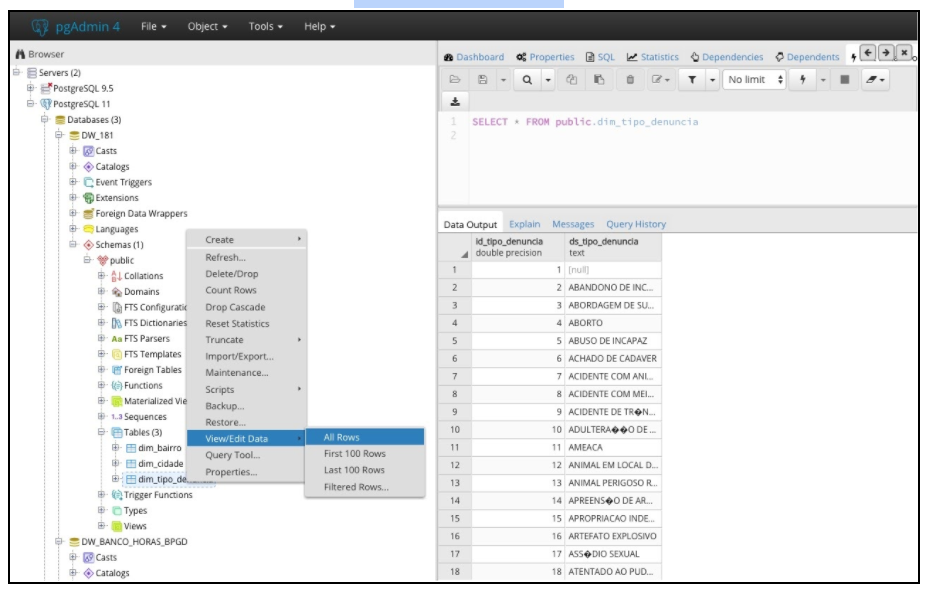
\includegraphics[width=0.6\textwidth]{./04-figuras/figura-res-tipo-denuncia}
    \label{fig:ilustfigrestipodenuncia}
\end{figure}
\vspace*{-0,9cm}
{\raggedright \fonte{Autor desta monografia, 2020.}} \\

% dim\_origem
\subsubsection{Criando a transforma\c{c}\~{a}o ``dim\_origem.ktr''}

Os componentes que far\~{a}o parte da transforma\c{c}\~{a}o ``dim\_origem.ktr'', ser\~{a}o: \textit{Microsoft Excel Input, Select values, Sort rows, Unique rows, Value Mapper, Add sequence} e finalmente \textit{Table Table output} conforme figura abaixo. 

\begin{figure}[H]
	\vspace*{0,2cm}
    \centering
    \caption{Transforma\c{c}\~{a}o ``dim\_origem.ktr'' do BI 181}
    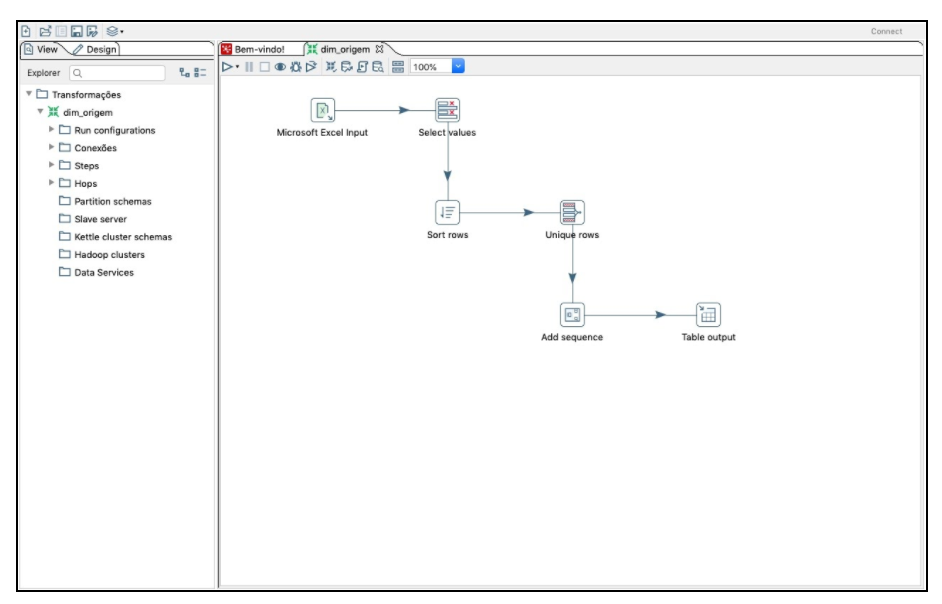
\includegraphics[width=0.6\textwidth]{./04-figuras/figura-dim-origem}
    \label{fig:ilustfigrdimorigem}
\end{figure}
\vspace*{-0,9cm}
{\raggedright \fonte{Autor desta monografia, 2020.}} \\

Primeiramente iremos configurar o \textit{step Select Value} (Selecione o Valor), e na aba \textit{Select and Alter}, na op\c{c}\~{a}o \textit{Fields, Rename to}, iremos modificar o nome Bairro para ``ds\_origem'', nesse componente ser\'{a} apenas essa a altera\c{c}\~{a}o, conforme figura da tela do \textit{step Select Value}.

Ap/'{o}s componente \textit{Select Value}, iremos configurar o \textit{step Sort rows} (Organizar a linha), na op\c{c}\~{a}o \textit{Fields, Ascending} como ``S'', para que os dados fiquem organizado de forma ascendente, figura da tela do \textit{step Sort rows}.

O pr/'{o}ximo componente \'{e} \textit{Unique rows} que tem a caracter\'{i}stica de selecionar apenas os valores únicos das linhas, ou seja, evitar a duplica\c{c}\~{a}o, nesse componente h\'{a} apenas a necessidade de configurar o nome do campo ou \textit{Fieldname}, conforma a figura da tela do \textit{step Unique rows}.

O componente \textit{Value Mapper}, em s\'{i}ntese tem como fun\c{c}\~{a}o trocar os valores vindos da linha da fonte de dados que ser\~{a}o comparados no \textit{Source Value}, e ap/'{o}s encontrar o mesmo ela ser\'{a} trocado pelo informado em \textit{Target value}, conforme a figura da tela do \textit{step Value Mapper}.

Ap/'{o}s transformarmos os dados brutos da linha ``origem'' da fonte de dado em \textit{Microsoft Excel}, iremos criar um campo sequencial, para isso usaremos o componente \textit{Add sequence}, a única altera\c{c}\~{a}o ser\'{a} no op\c{c}\~{a}o Nome do valor, que foi mudado para ``id\_origem'', conforme figura na tela do \textit{Add sequence}.

Finalizando a transforma\c{c}\~{a}o ``dim\_origem.ktr'', usaremos o componente \textit{Table output} nele iremos alterar as op\c{c}\~{o}es \textit{Connection, Target schema, Target table, truncate table}, e na aba \textit{Database fields}, incluiremos os Campos ou colunas da tabela ``dim\_origem'' que ser\'{a} criada ap/'{o}s finalizar essa etapa de configura\c{c}\~{a}o dos componentes da transforma\c{c}\~{a}o, conforme a figura da tela do \textit{step Table output}.

\begin{figure}[H]
	\vspace*{0,2cm}
    \centering
    \caption{Configurando os \textit{steps} da Transforma\c{c}\~{a}o ``dim\_origem.ktr'' (passo-a-passo)}
    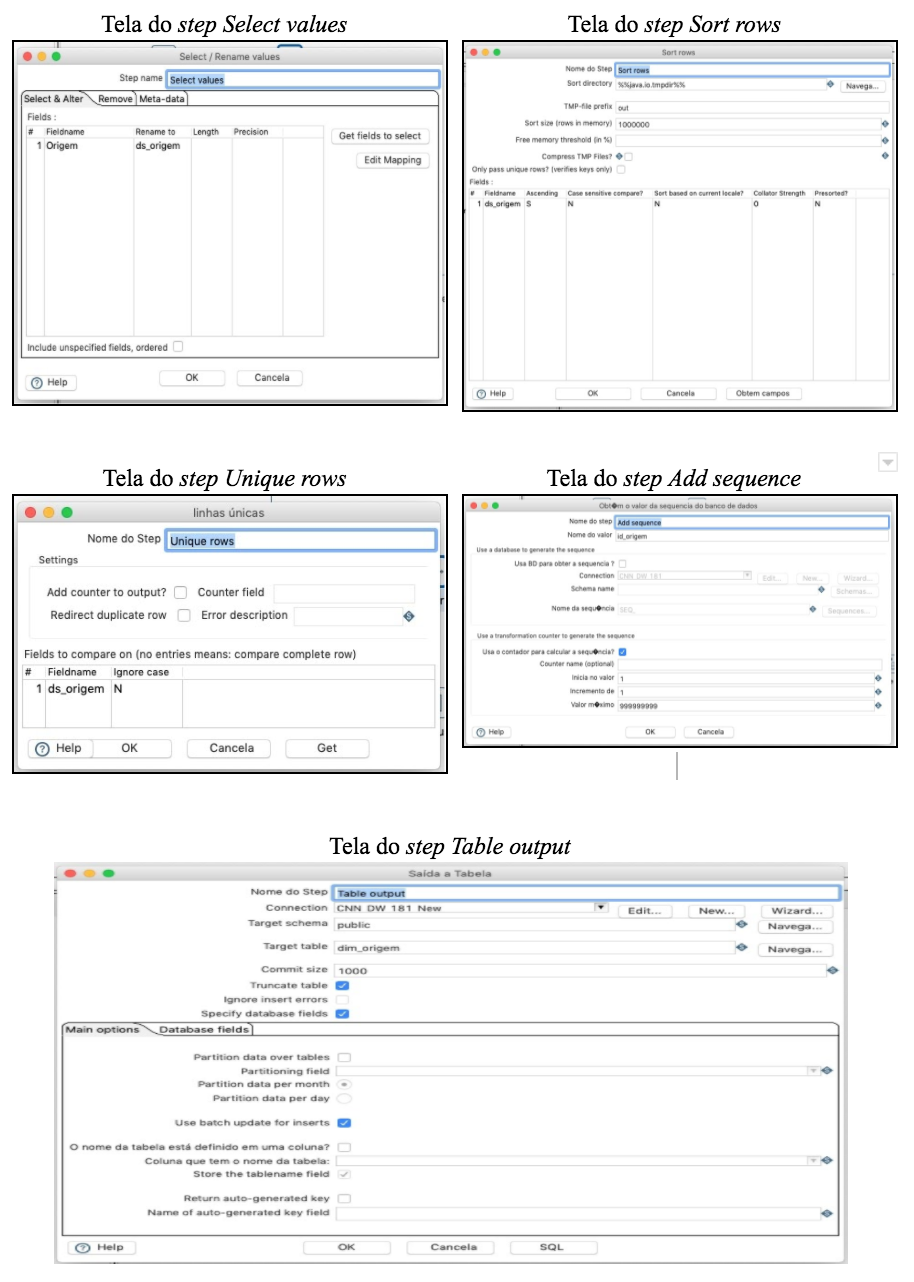
\includegraphics[width=0.6\textwidth]{./04-figuras/figura-dim-origem-passo-a-passo}
    \label{fig:ilustfigdimorigempassoapasso}
\end{figure}
\vspace*{-0,9cm}
{\raggedright \fonte{Autor desta monografia, 2020.}} \\

\begin{figure}[H]
	\vspace*{0,2cm}
    \centering
    \caption{Criando a tabela ``dim\_origem'' no banco de dados usando o \textit{step Table output}}
    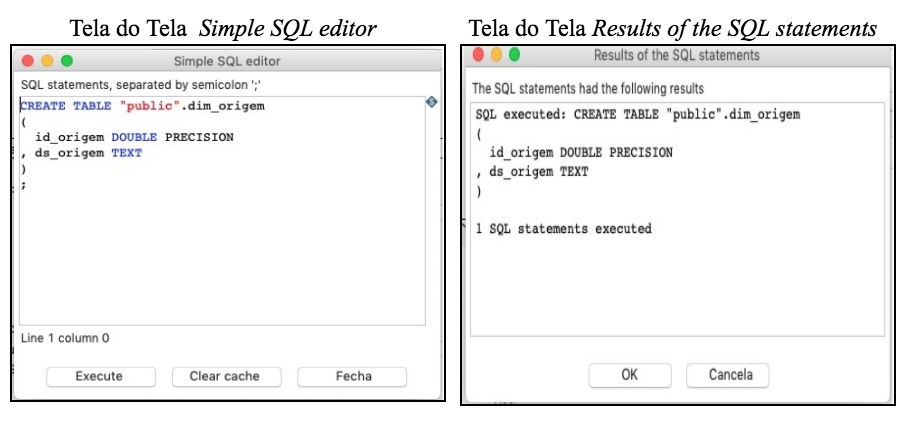
\includegraphics[width=0.6\textwidth]{./04-figuras/figura-tb-dim-origem}
    \label{fig:ilustfigtbdimorigem}
\end{figure}
\vspace*{-0,9cm}
{\raggedright \fonte{Autor desta monografia, 2020.}} \\

Ao final dos processos quando executamos a transforma\c{c}\~{a}o, conforme figura 53, na parte posterior da tela do PDI, em ``Execution Results''. aparecer\'{a} na aba ``Preview data'', os dados padronizados dos campos: ``id\_origem'' e ``ds\_origem''. O pr/'{o}ximo passo ser\'{a} percorrer a grade com os resultado e perceber se o processo de transforma\c{c}\~{a}o e carga sai conforme planejado. 

\begin{figure}[H]
	\vspace*{0,2cm}
    \centering
    \caption{Executando a transforma\c{c}\~{a}o ``dim\_origem.ktr''}
    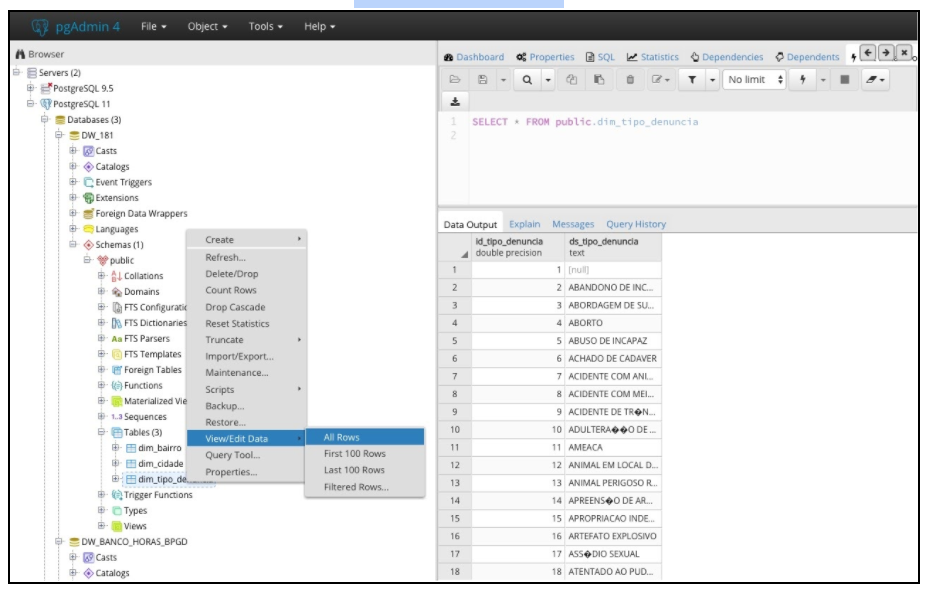
\includegraphics[width=0.6\textwidth]{./04-figuras/figura-res-tipo-denuncia}
    \label{fig:ilustfigrestipodenuncia}
\end{figure}
\vspace*{-0,9cm}
{\raggedright \fonte{Autor desta monografia, 2020.}} \\

Para se ter certeza de que a tabela ``dim\_origem'', obteve a ETL correta, precisamos abrir a tabela ``dim\_origem'' no aplicativo pgAdmin4, que \'{e} instalado junto ao PostgreSQL, conforme figura abaixo, nela podemos analisar os dados processados pela transforma\c{c}\~{a}o criada no PDI: ``dim\_origem.ktr''.

\begin{figure}[H]
	\vspace*{0,2cm}
    \centering
    \caption{Resultado da transforma\c{c}\~{a}o e carga no Banco de Dados ``DW\_181'' na tabela ``dim\_origem''}
    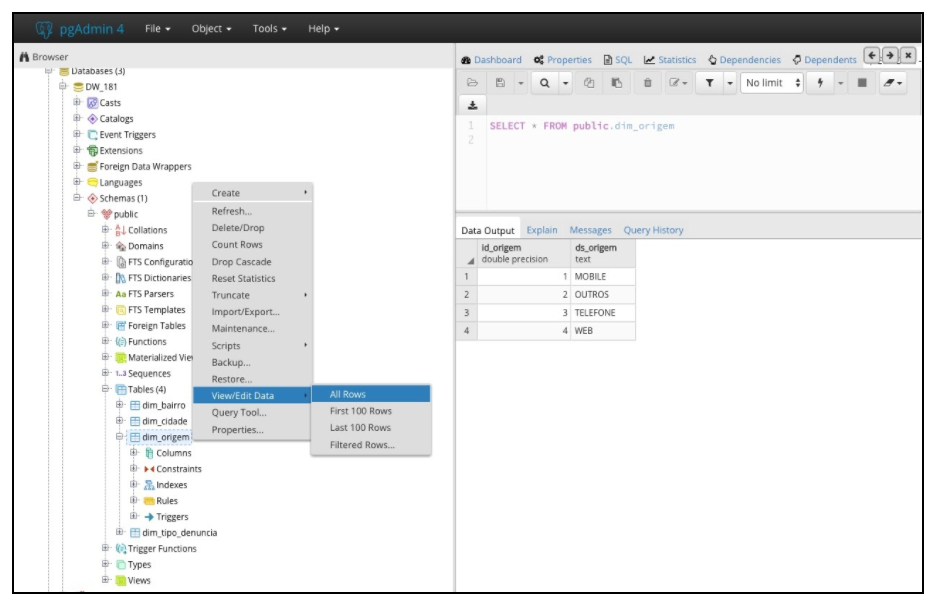
\includegraphics[width=0.6\textwidth]{./04-figuras/figura-res-dim-origem}
    \label{fig:ilustfigresdimorigem}
\end{figure}
\vspace*{-0,9cm}
{\raggedright \fonte{Autor desta monografia, 2020.}} \\

% TRANSFORMA\C{C}\~{A}O DIM\_DATA.KTL
\subsubsection{Criando a transforma\c{c}\~{a}o ``dim\_data.ktr''}

Diferente das transforma\c{c}\~{o}es dos t\'{o}picos anteriores, a transforma\c{c}\~{a}o ``dim\_data.ktr'', 
\'{e} muito mais complexa, nela iremos usar componentes de step, como o Calculator e o String cut. 
Na figura abaixo, podemos perceber que esta transforma\c{c}\~{a}o tem como prioridade criar 
as tabelas ``dim\_dia'', ``dim\_semana'', ``dim\_mes'', ``dim\_trimestre'', ``dim\_semestre'' e 
a ``dim\_ano'', ao final de todo processo iremos produzir um DW, e criar an\'{a}lises que podem 
usar essas dimens\~{o}es/tabelas.
Iremos, passo a passo e atrav\'{e}s de figuras construir a ETL da transforma\c{c}\~{a}o ``dim\_data.ktr''.

\begin{figure}[H]
	\vspace*{0,2cm}
    \centering
    \caption{Transforma\c{c}\~{a}o ``dim\_data.ktr'' do BI 181}
    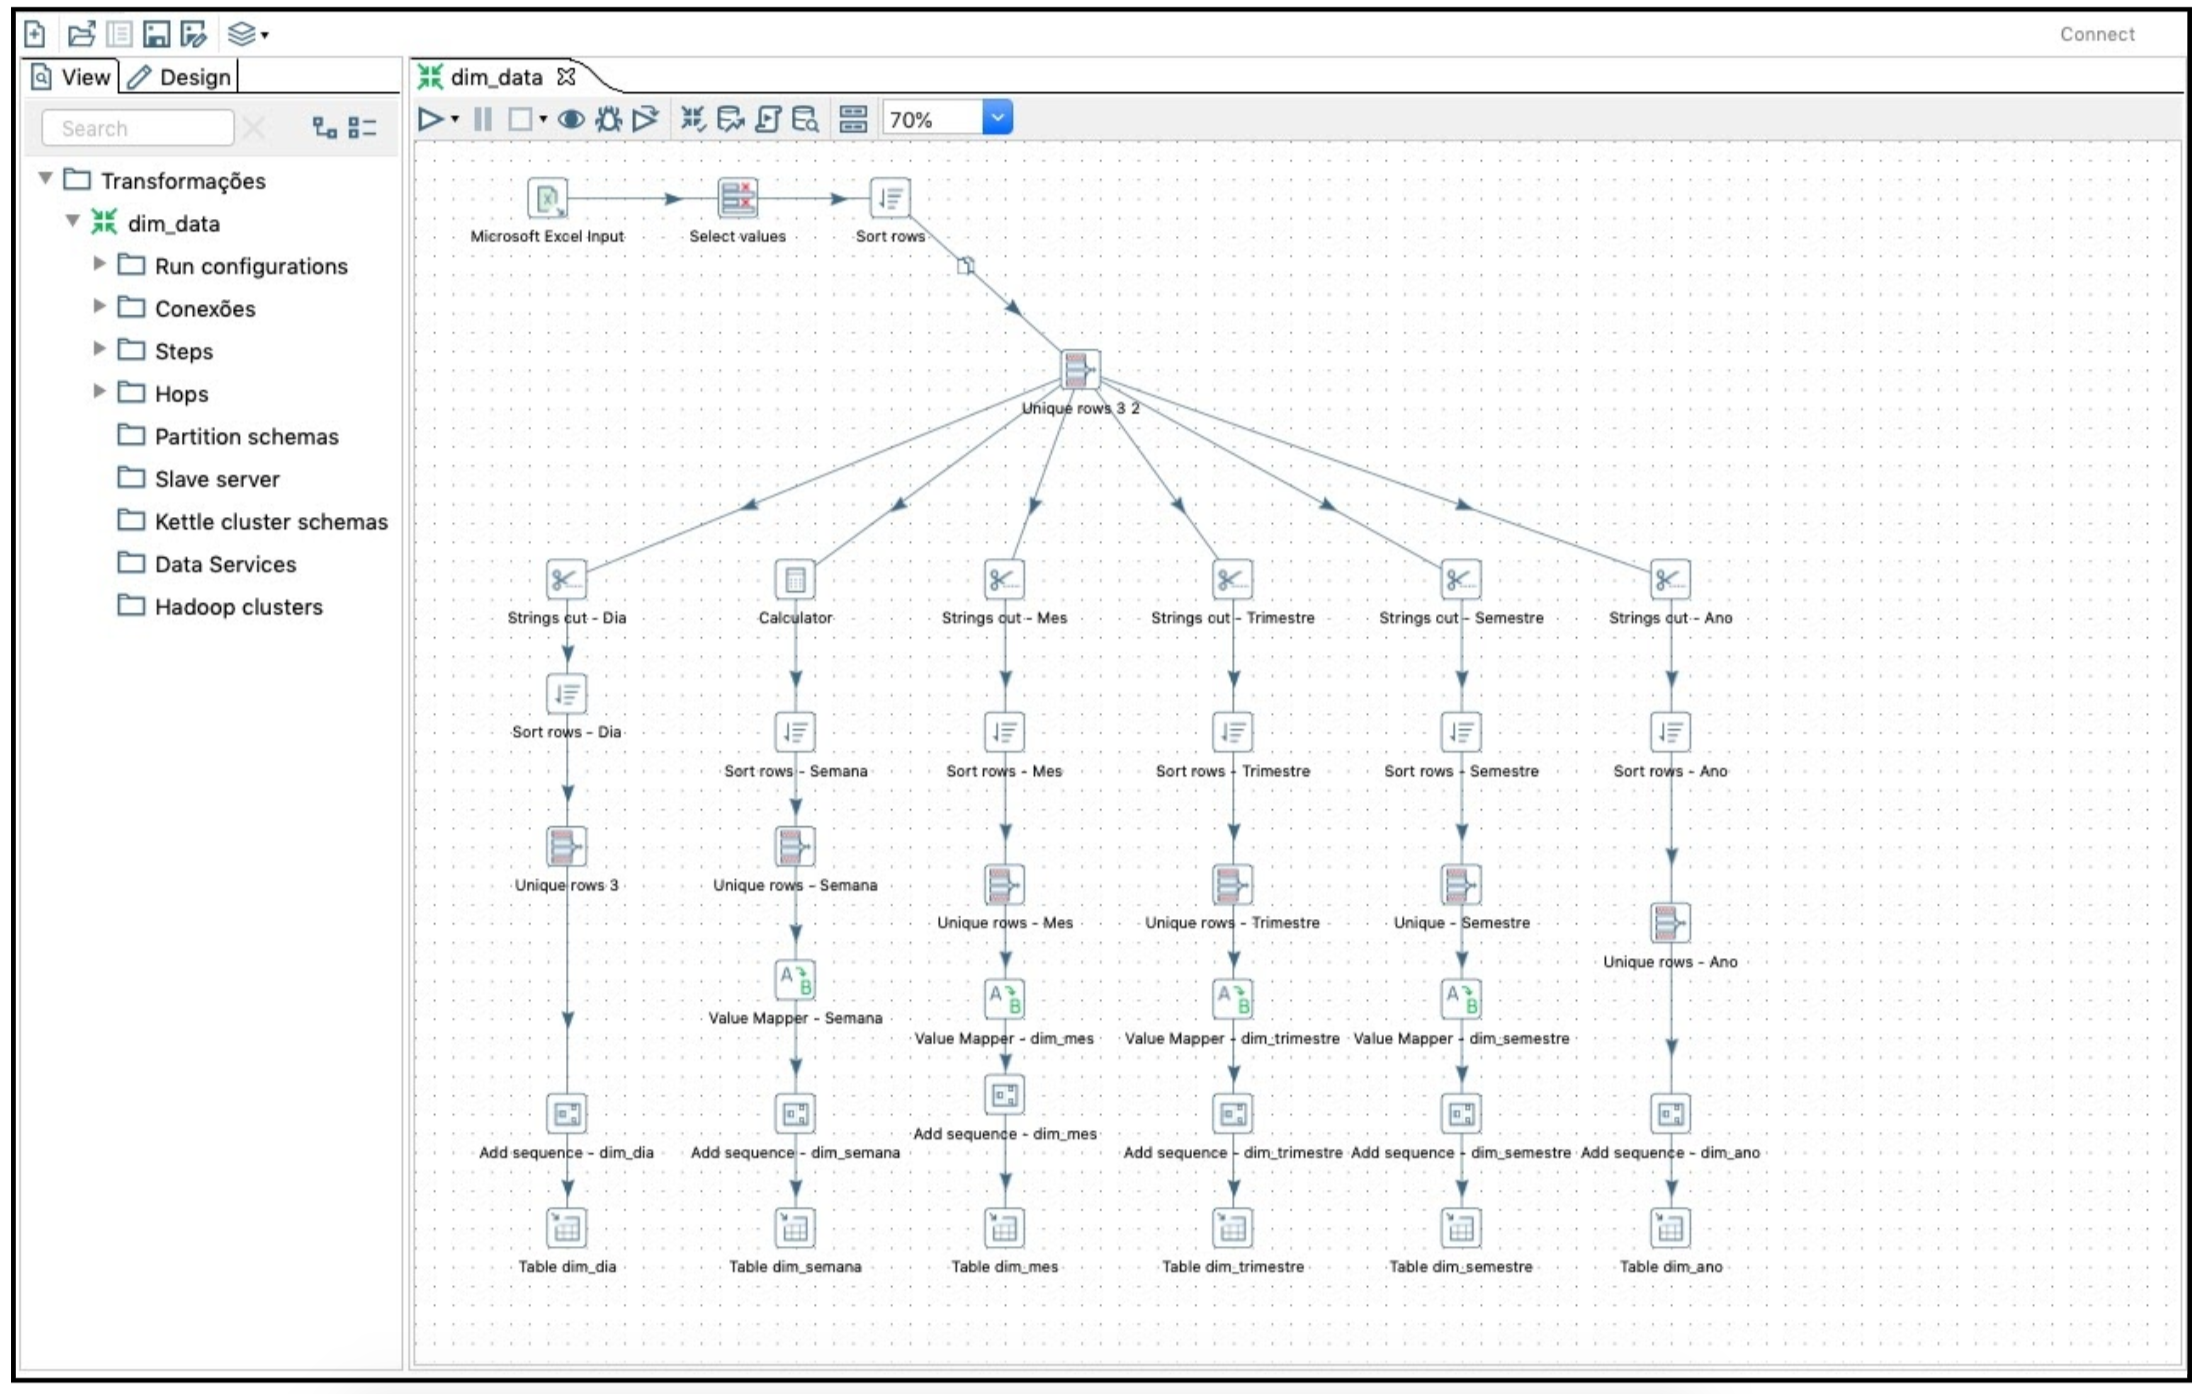
\includegraphics[width=0.6\textwidth]{./04-figuras/figura-dim-data}
    \label{fig:ilustfigresdimdata}
\end{figure}
\vspace*{-0,9cm}
{\raggedright \fonte{Autor desta monografia, 2020.}} \\

Na figura abaixo, temos o esquema da transforma\c{c}\~{a}o ``dim\_data'', composta pelos componentes: 
\textit{Select values, Sort rows, String Cut, Calculator, Unique rows, Add sequence, Table output}. 
A novidade nessa transforma\c{c}\~{a}o s\~{a}o os steps: \textit{String Cut, Calculator} e o movimento de dados 
entre o \textit{step Sort rows} e o \textit{Unique rows 2 2}, conforme a figura abaixo que apresenta um 
pequeno \'{i}cone de c\'{o}pia, que na verdade, sai do padr\~{a}o da configura\c{c}\~{a}o b\'{a}sica, que \'{e} o movimento
de dados, pelo m\'{e}todo \textit{Round-robin}\index{RoundRobin}\footnote{Round-robin s\~{a}o estas etapas que ser\~{a}o 
executadas em paralelo, o padr\~{a}o nas transforma\c{c}\~{o}es do PDI, e n\~{a}o de uma forma sequencial como na dados para os pr\'{o}ximos steps. 
} de cada \textit{step} entre seu \textit{hop} e o pr\'{o}ximo \textit{step}, sem configurar para ``copia dados para os pr\'{o}ximos steps'' 
os dados transformados para cada dimens\~{a}o n\~{a}o trar\'{a} o resultado esperado ao final do processo.

Nas figuras abaixo que se seguem para cada ramifica\c{c}\~{a}o temos a cria\c{c}\~{a}o das dimens\~{o}es que a transforma\c{c}\~{a}o 
``dim\_data.ktr'' ir\~{a} criar como as: dim\_dia, dim\_semana, dim\_mes, dim\_trimestre, 
dim\_semestre e dim\_ano, iremos desvendar a particularidade de cada uma, 
pois, quando estivermos analisando os dados ao final desse trabalho teremos 
um entendimento melhor da fun\c{c}\~{a}o de cada dimens\~{a}o aqui desenvolvida dentro do contexto do BI.

% dim\_data.ktr
\begin{figure}[H]
	\vspace*{0,2cm}
    \centering
    \caption{Configurando os \textit{steps} da Transforma\c{c}\~{a}o ``dim\_data.ktr'' na ramifica\c{c}\~{a}o principal}
    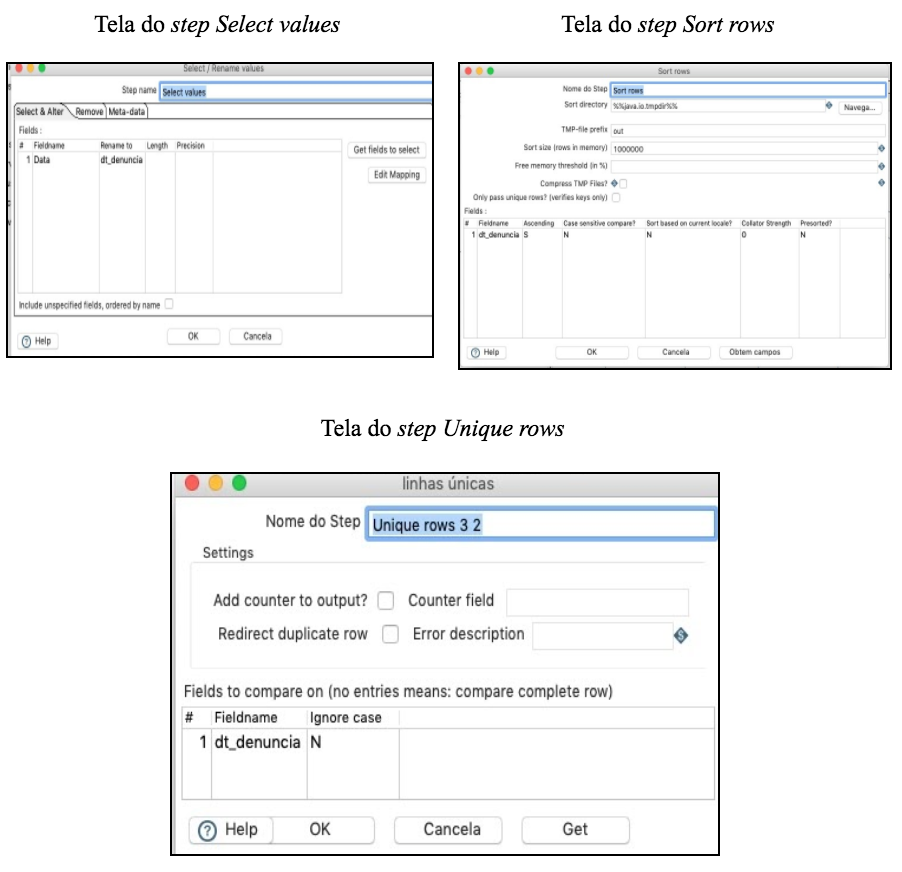
\includegraphics[width=0.6\textwidth]{./04-figuras/figura-dim-data-steps.png}
    \label{fig:ilustfigdimdatasteps}
\end{figure}
\vspace*{-0,9cm}
{\raggedright \fonte{Autor desta monografia, 2020.}} \\

% dim\_dia
\begin{figure}[H]
	\vspace*{0,2cm}
    \centering
    \caption{Criando a tabela ``dim\_dia'' atrav\'{e}s da Transforma\c{c}\~{a}o ``dim\_data.ktr''}
    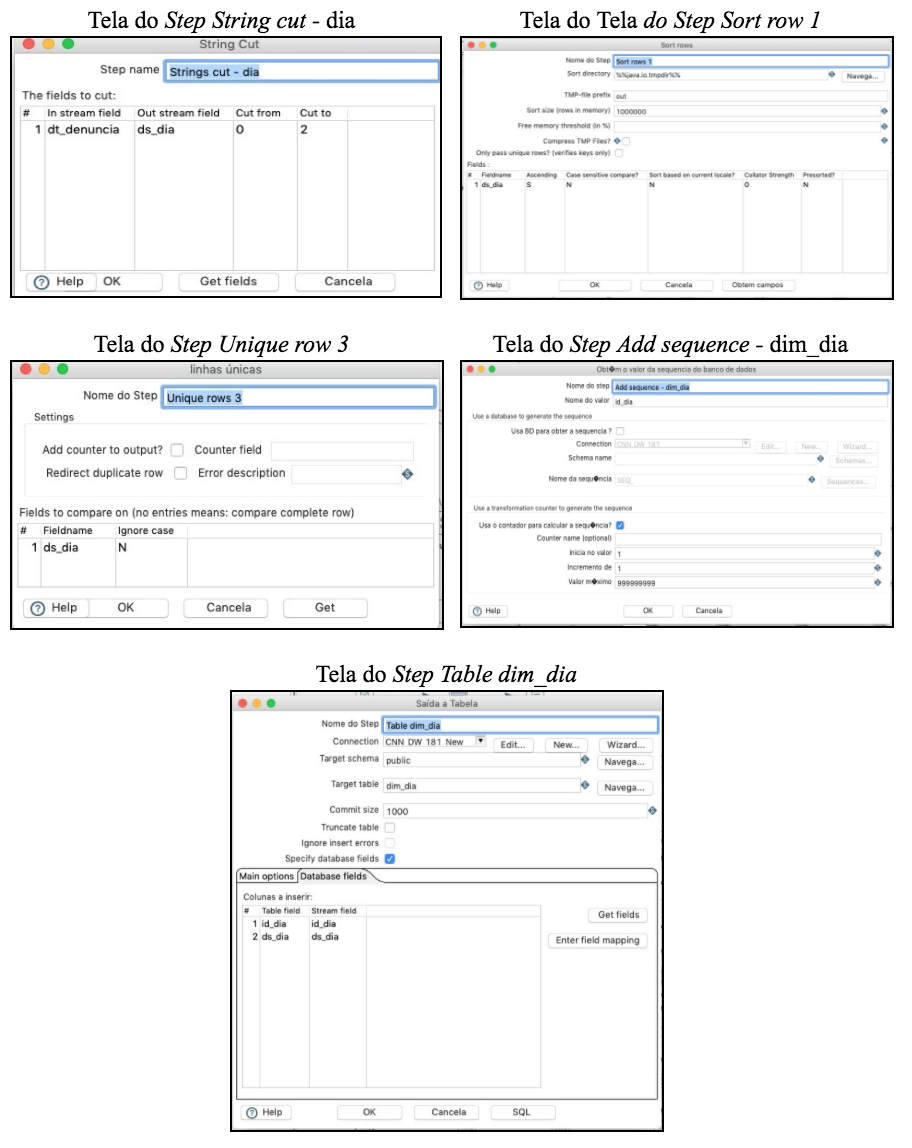
\includegraphics[width=0.6\textwidth]{./04-figuras/figura-dim-dia}
    \label{fig:ilustfigdimdia}
\end{figure}
\vspace*{-0,9cm}
{\raggedright \fonte{Autor desta monografia, 2020.}} \\

\begin{figure}[H]
	\vspace*{0,2cm}
    \centering
    \caption{Criando a tabela ``dim\_dia'' no banco de dados usando o \textit{step Table} dim\_dia}
    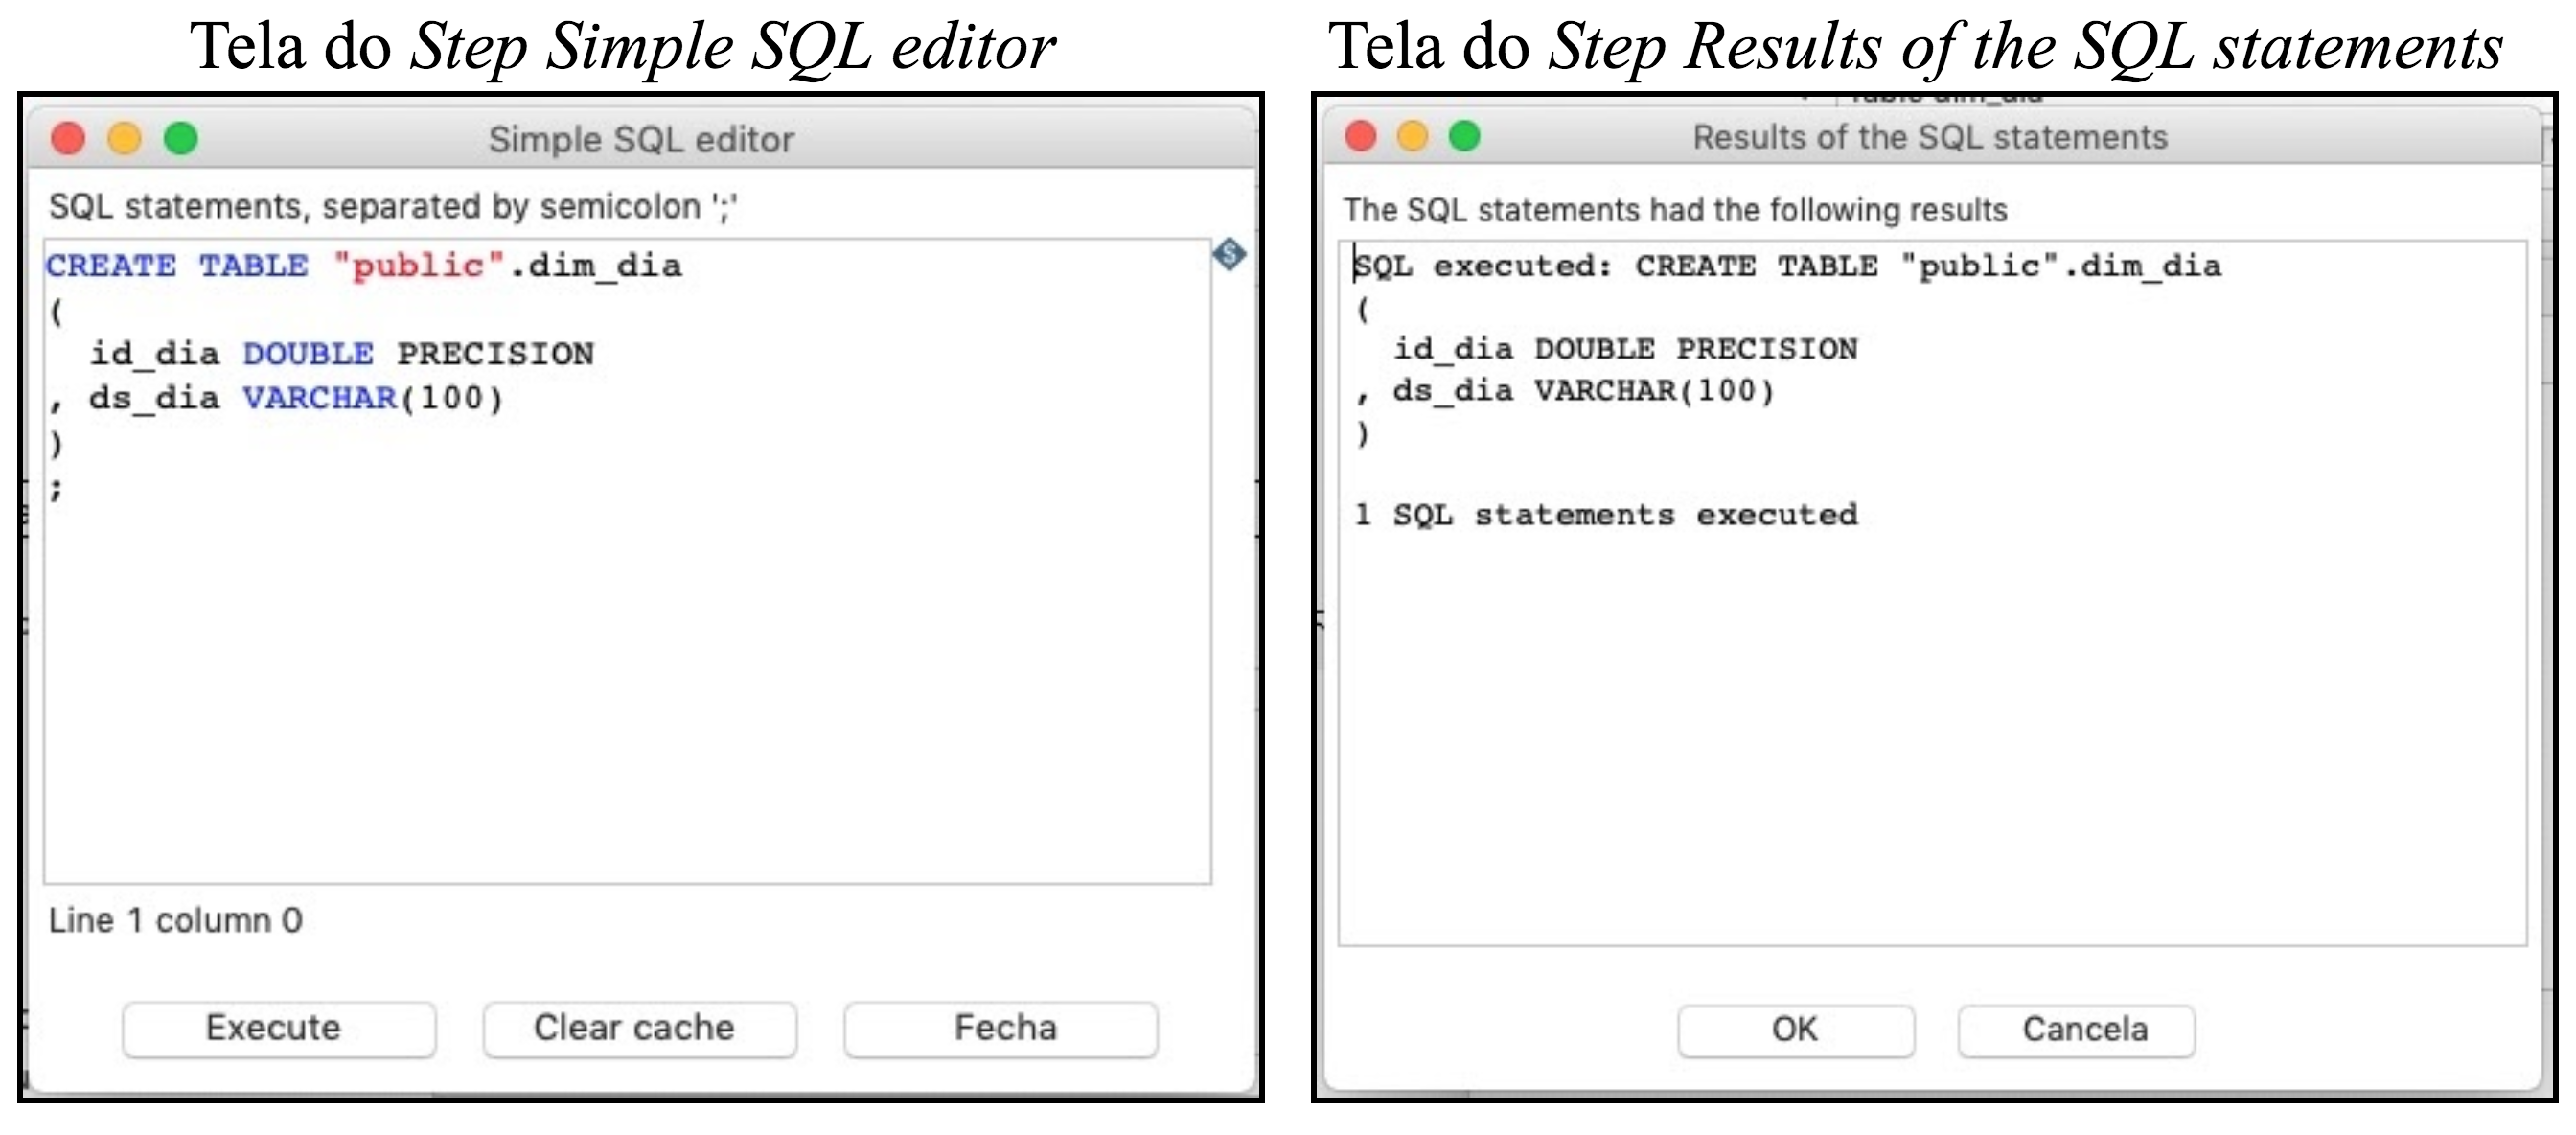
\includegraphics[width=0.6\textwidth]{./04-figuras/figura-tb-dim-dia}
    \label{fig:ilustfigtbdimdia}
\end{figure}
\vspace*{-0,9cm}
{\raggedright \fonte{Autor desta monografia, 2020.}} \\

% dim\_semana
\begin{figure}[H]
	\vspace*{0,2cm}
    \centering
    \caption{Criando a tabela ``dim\_semana'' atrav\'{e}s da Transforma\c{c}\~{a}o ``dim\_data.ktr''}
    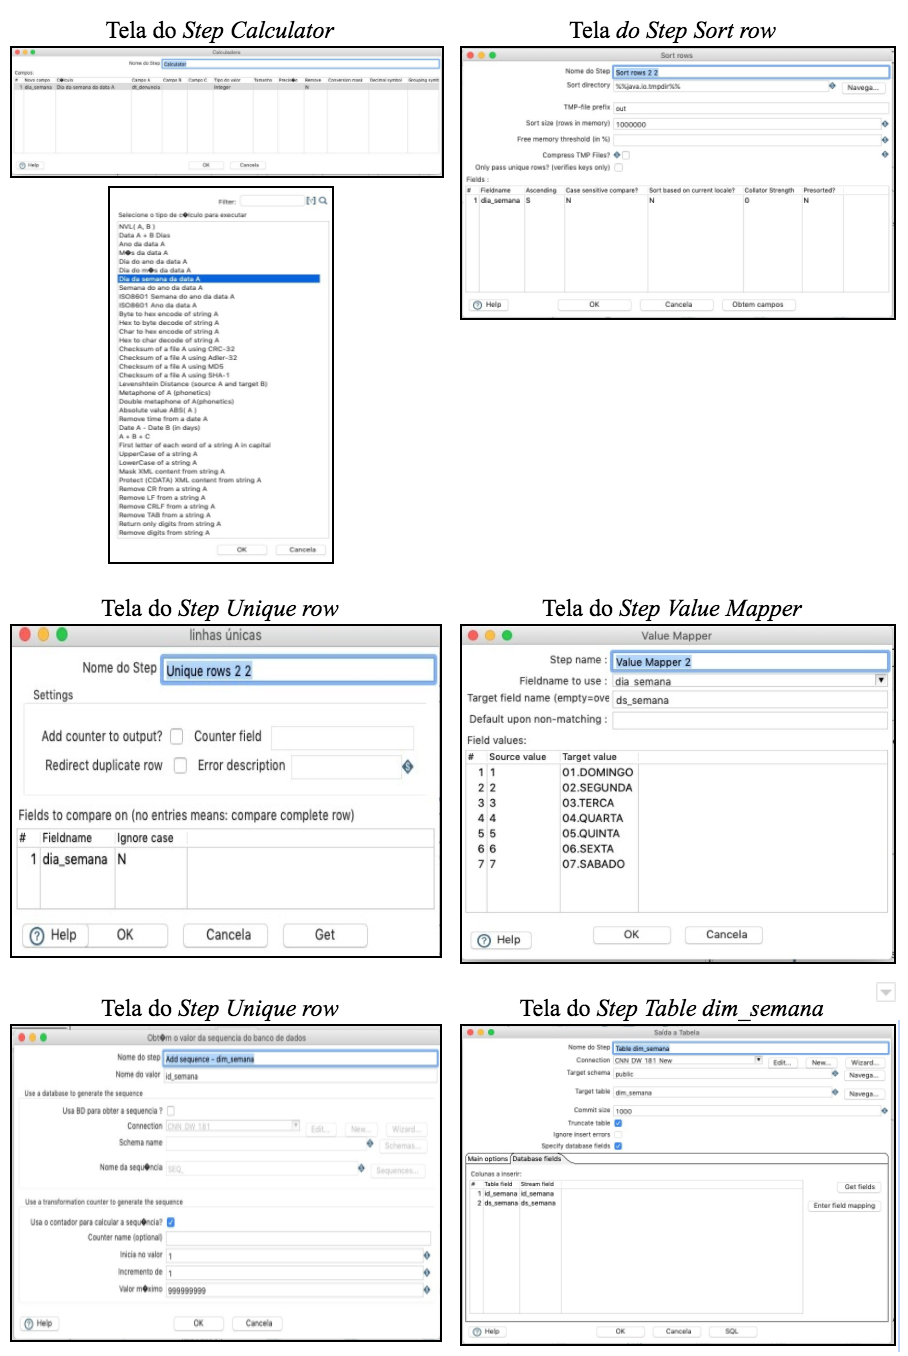
\includegraphics[width=0.6\textwidth]{./04-figuras/figura-dim-semana}
    \label{fig:ilustfigdimsemana}
\end{figure}
\vspace*{-0,9cm}
{\raggedright \fonte{Autor desta monografia, 2020.}} \\

\begin{figure}[H]
	\vspace*{0,2cm}
    \centering
    \caption{Criando a tabela ``dim\_semana'' no banco de dados usando o \textit{step Table} dim\_semana}
    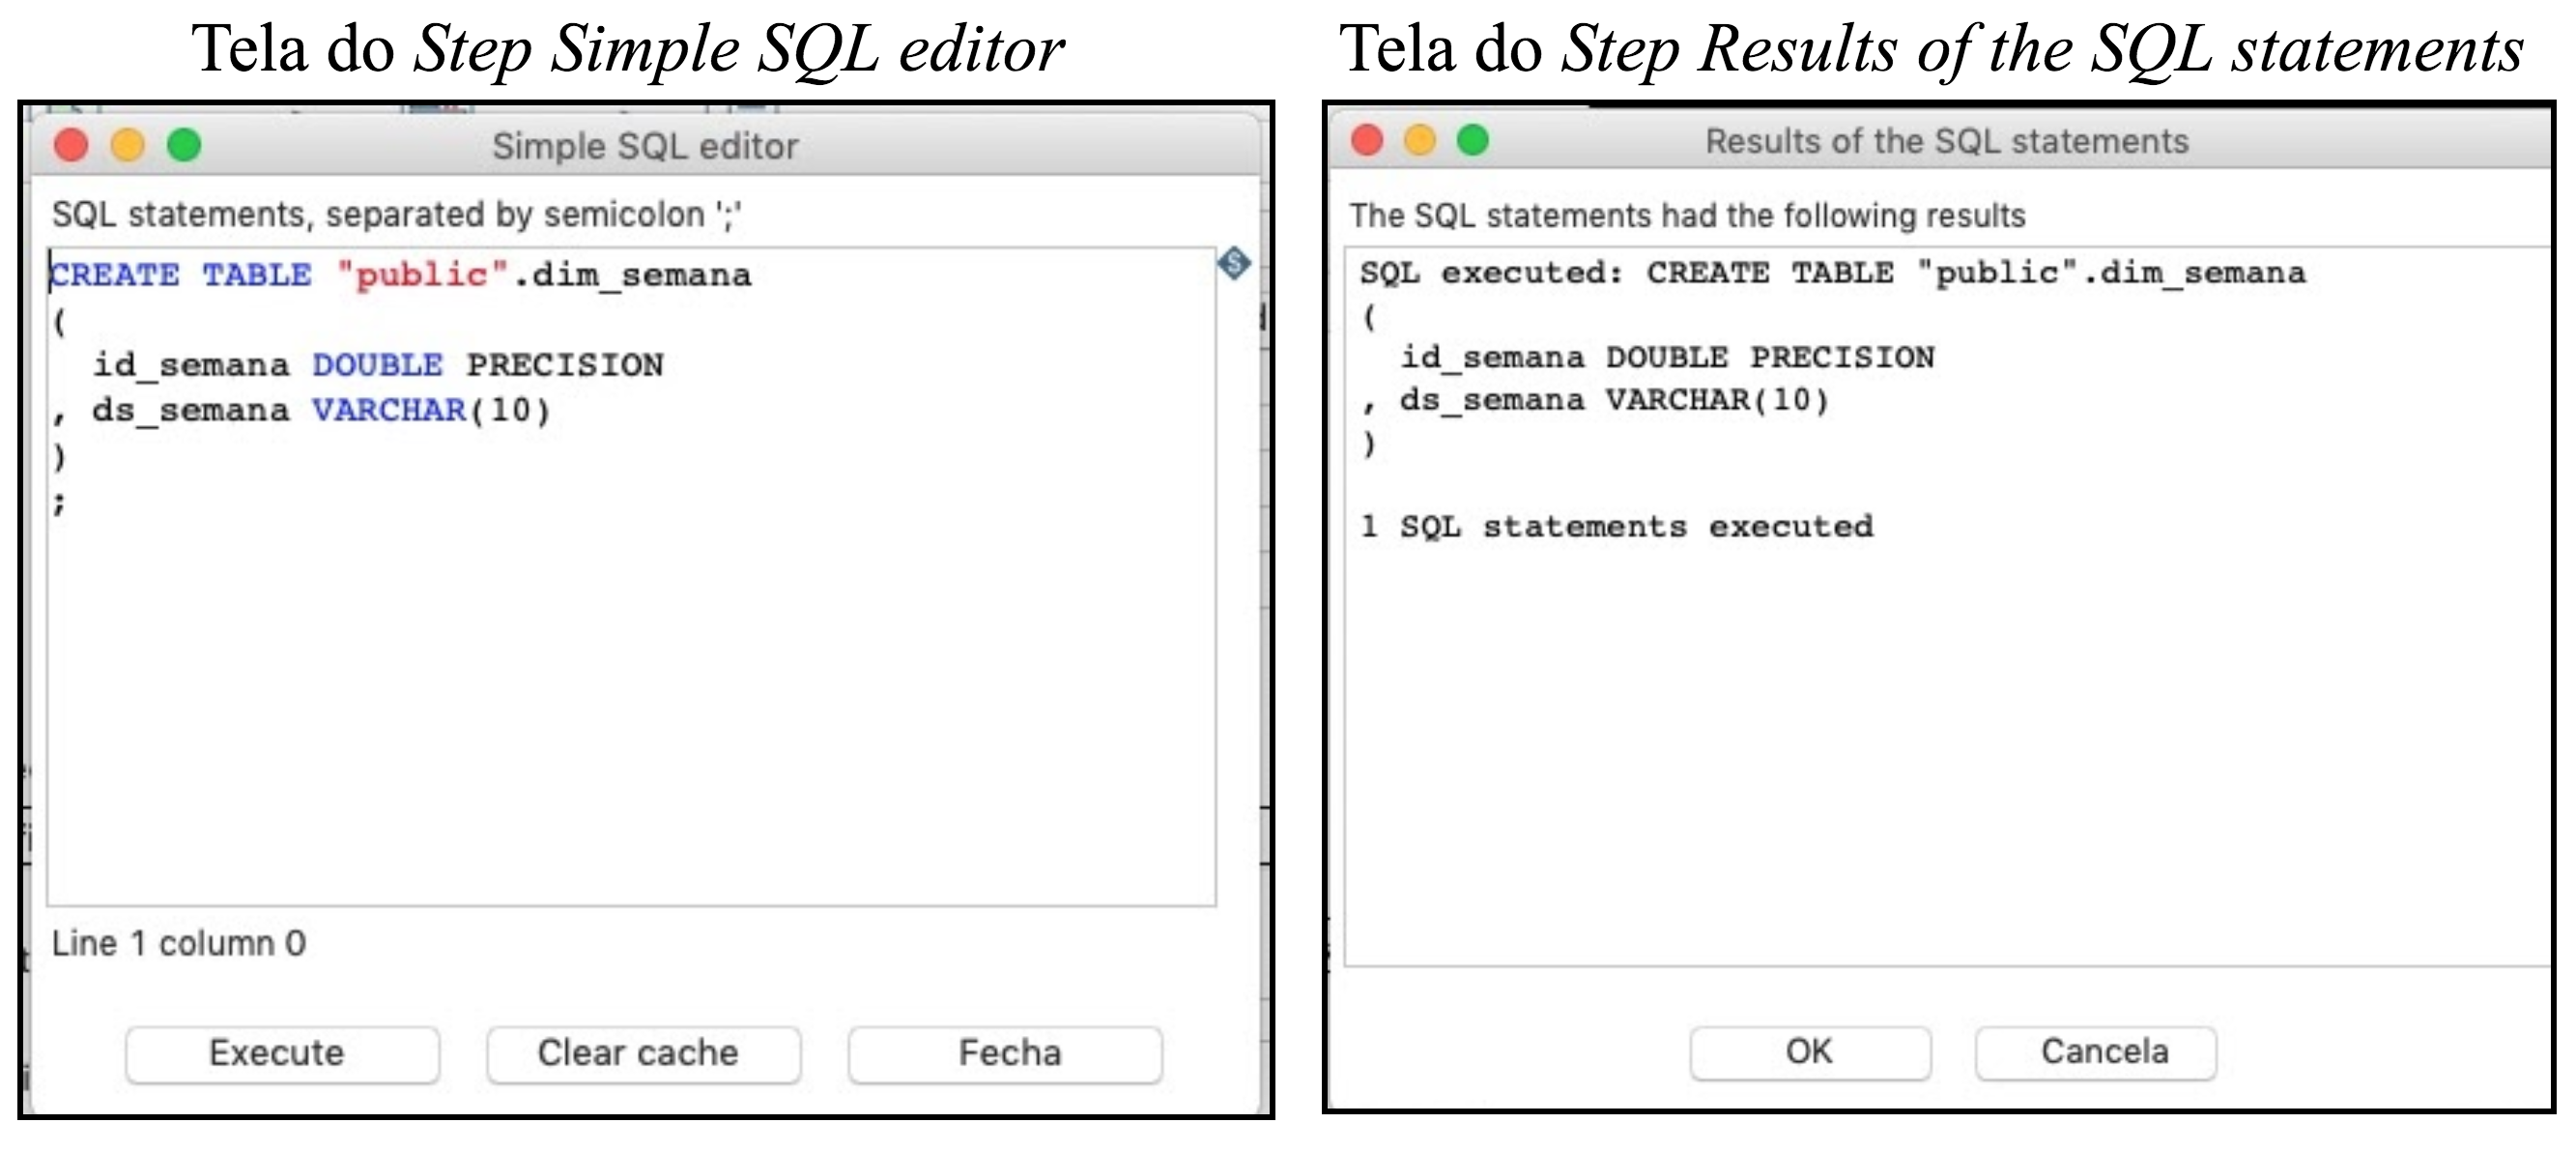
\includegraphics[width=0.6\textwidth]{./04-figuras/figura-tb-dim-semana}
    \label{fig:ilustfigtbdimsemana}
\end{figure}
\vspace*{-0,9cm}
{\raggedright \fonte{Autor desta monografia, 2020.}} \\

% dim\_mes
\begin{figure}[H]
	\vspace*{0,2cm}
    \centering
    \caption{Criando a tabela ``dim\_mes`` atrav\'{e}s da Transforma\c{c}\~{a}o ``dim\_data.ktr''}
    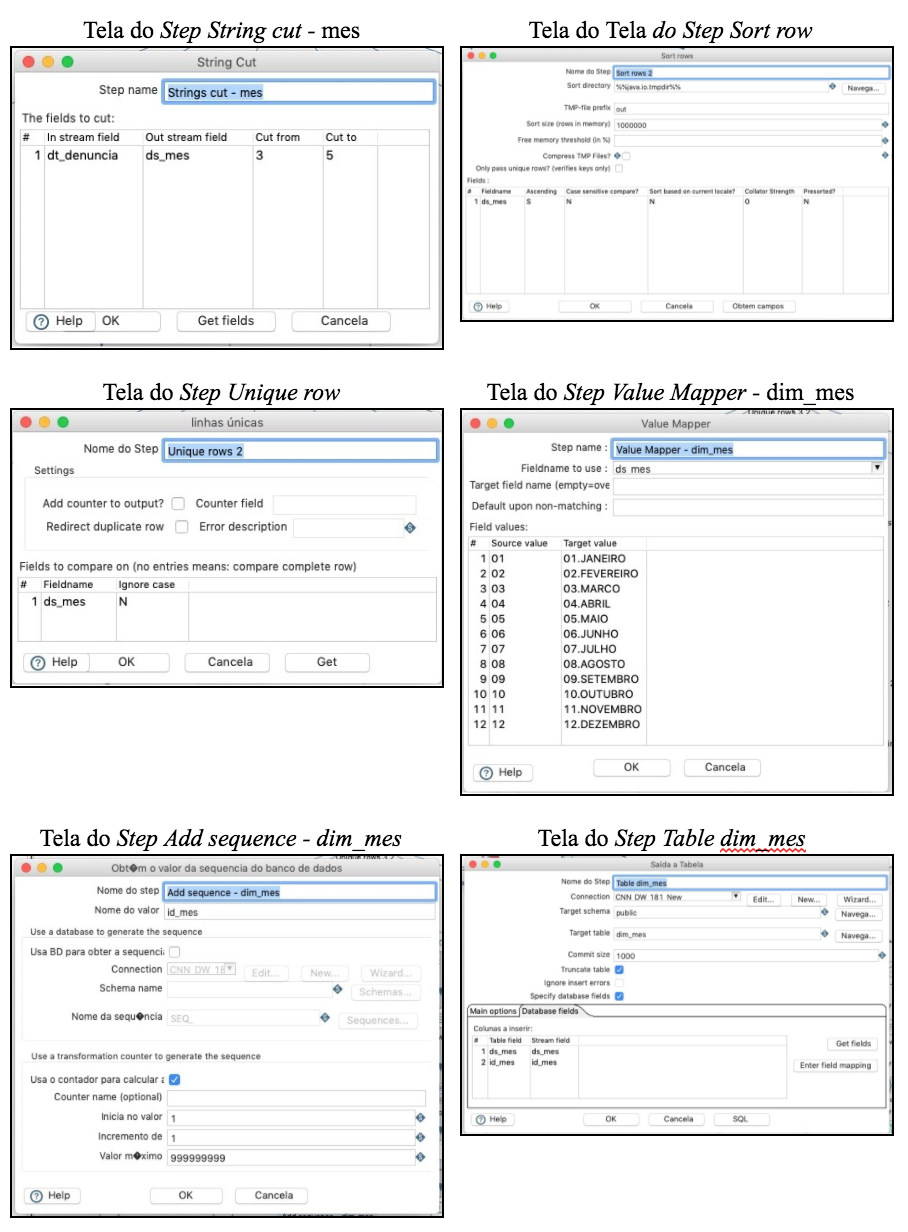
\includegraphics[width=0.6\textwidth]{./04-figuras/figura-dim-mes}
    \label{fig:ilustfigdimmes}
\end{figure}
\vspace*{-0,9cm}
{\raggedright \fonte{Autor desta monografia, 2020.}} \\

\begin{figure}[H]
	\vspace*{0,2cm}
    \centering
    \caption{Criando a tabela ``dim\_semana'' no banco de dados usando o \textit{step Table} dim\_semana}
    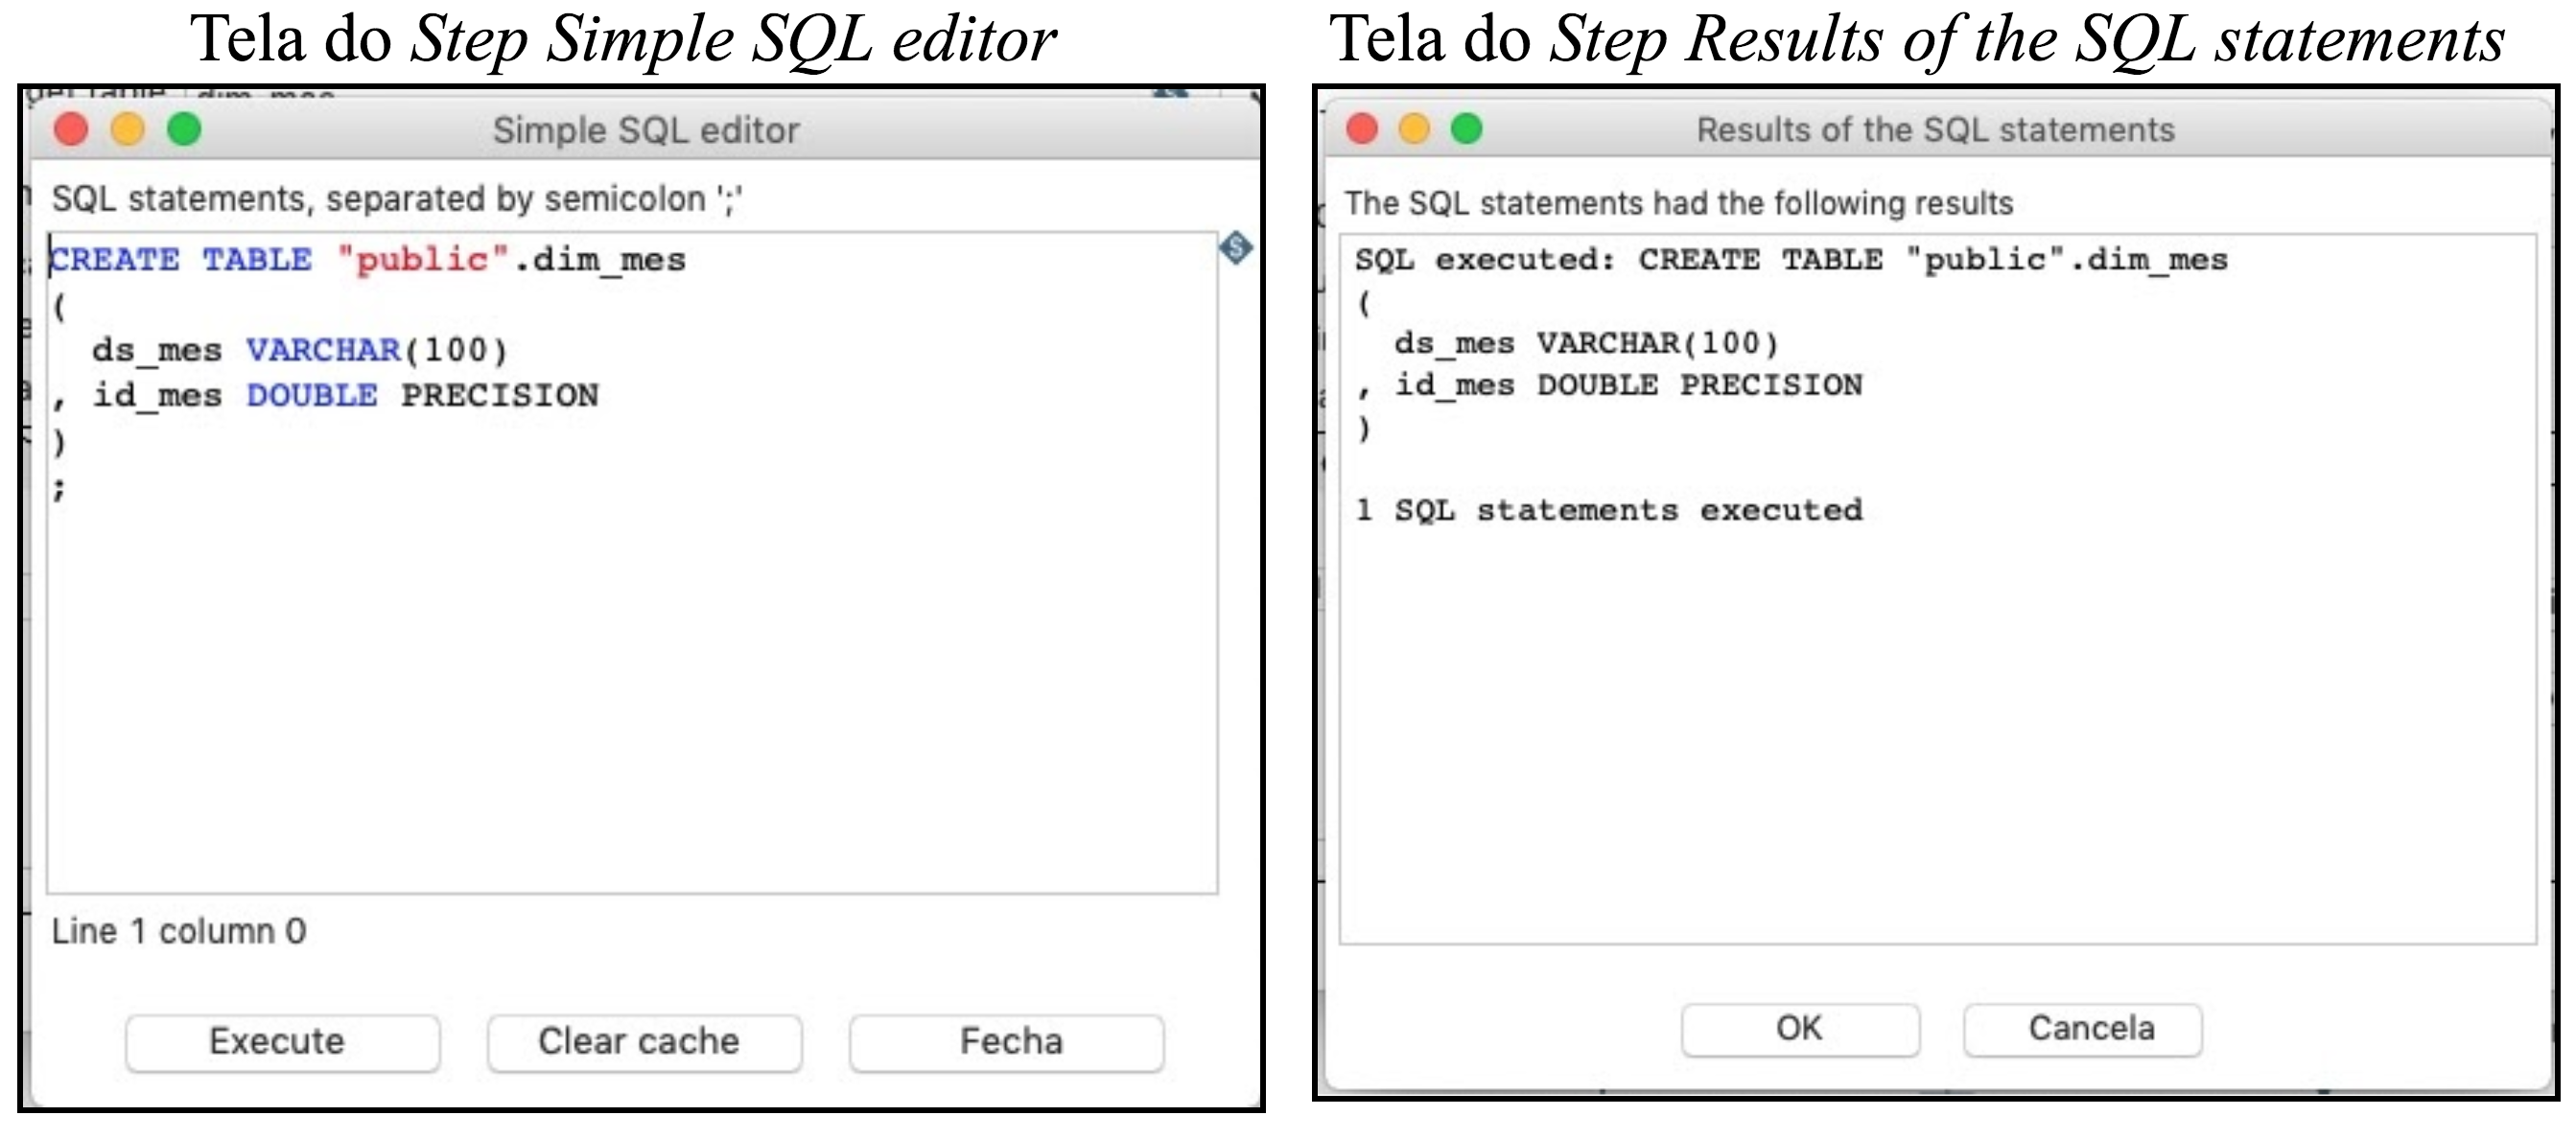
\includegraphics[width=0.6\textwidth]{./04-figuras/figura-tb-dim-mes}
    \label{fig:ilustfigtbdimmes}
\end{figure}
\vspace*{-0,9cm}
{\raggedright \fonte{Autor desta monografia, 2020.}} \\

% dim\_trimestre
\begin{figure}[H]
	\vspace*{0,2cm}
    \centering
    \caption{Criando a tabela ``dim\_trimestre`` atrav\'{e}s da Transforma\c{c}\~{a}o ``dim\_data.ktr''}
    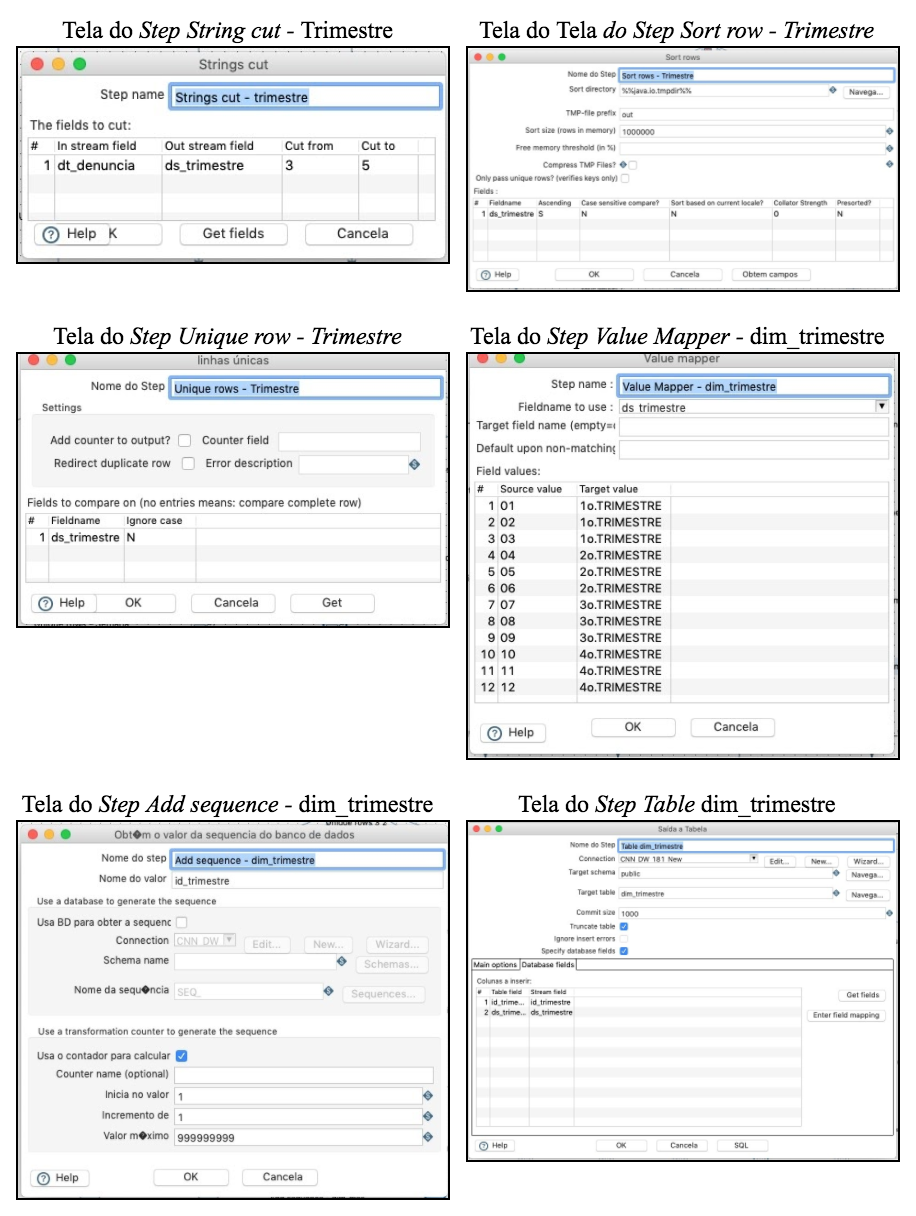
\includegraphics[width=0.6\textwidth]{./04-figuras/figura-dim-trimestre}
    \label{fig:ilustfigdimtrimestre}
\end{figure}
\vspace*{-0,9cm}
{\raggedright \fonte{Autor desta monografia, 2020.}} \\

\begin{figure}[H]
	\vspace*{0,2cm}
    \centering
    \caption{Criando a tabela ``dim\_trimestre`` no banco de dados usando o \textit{step Table} dim\_trimestre}
    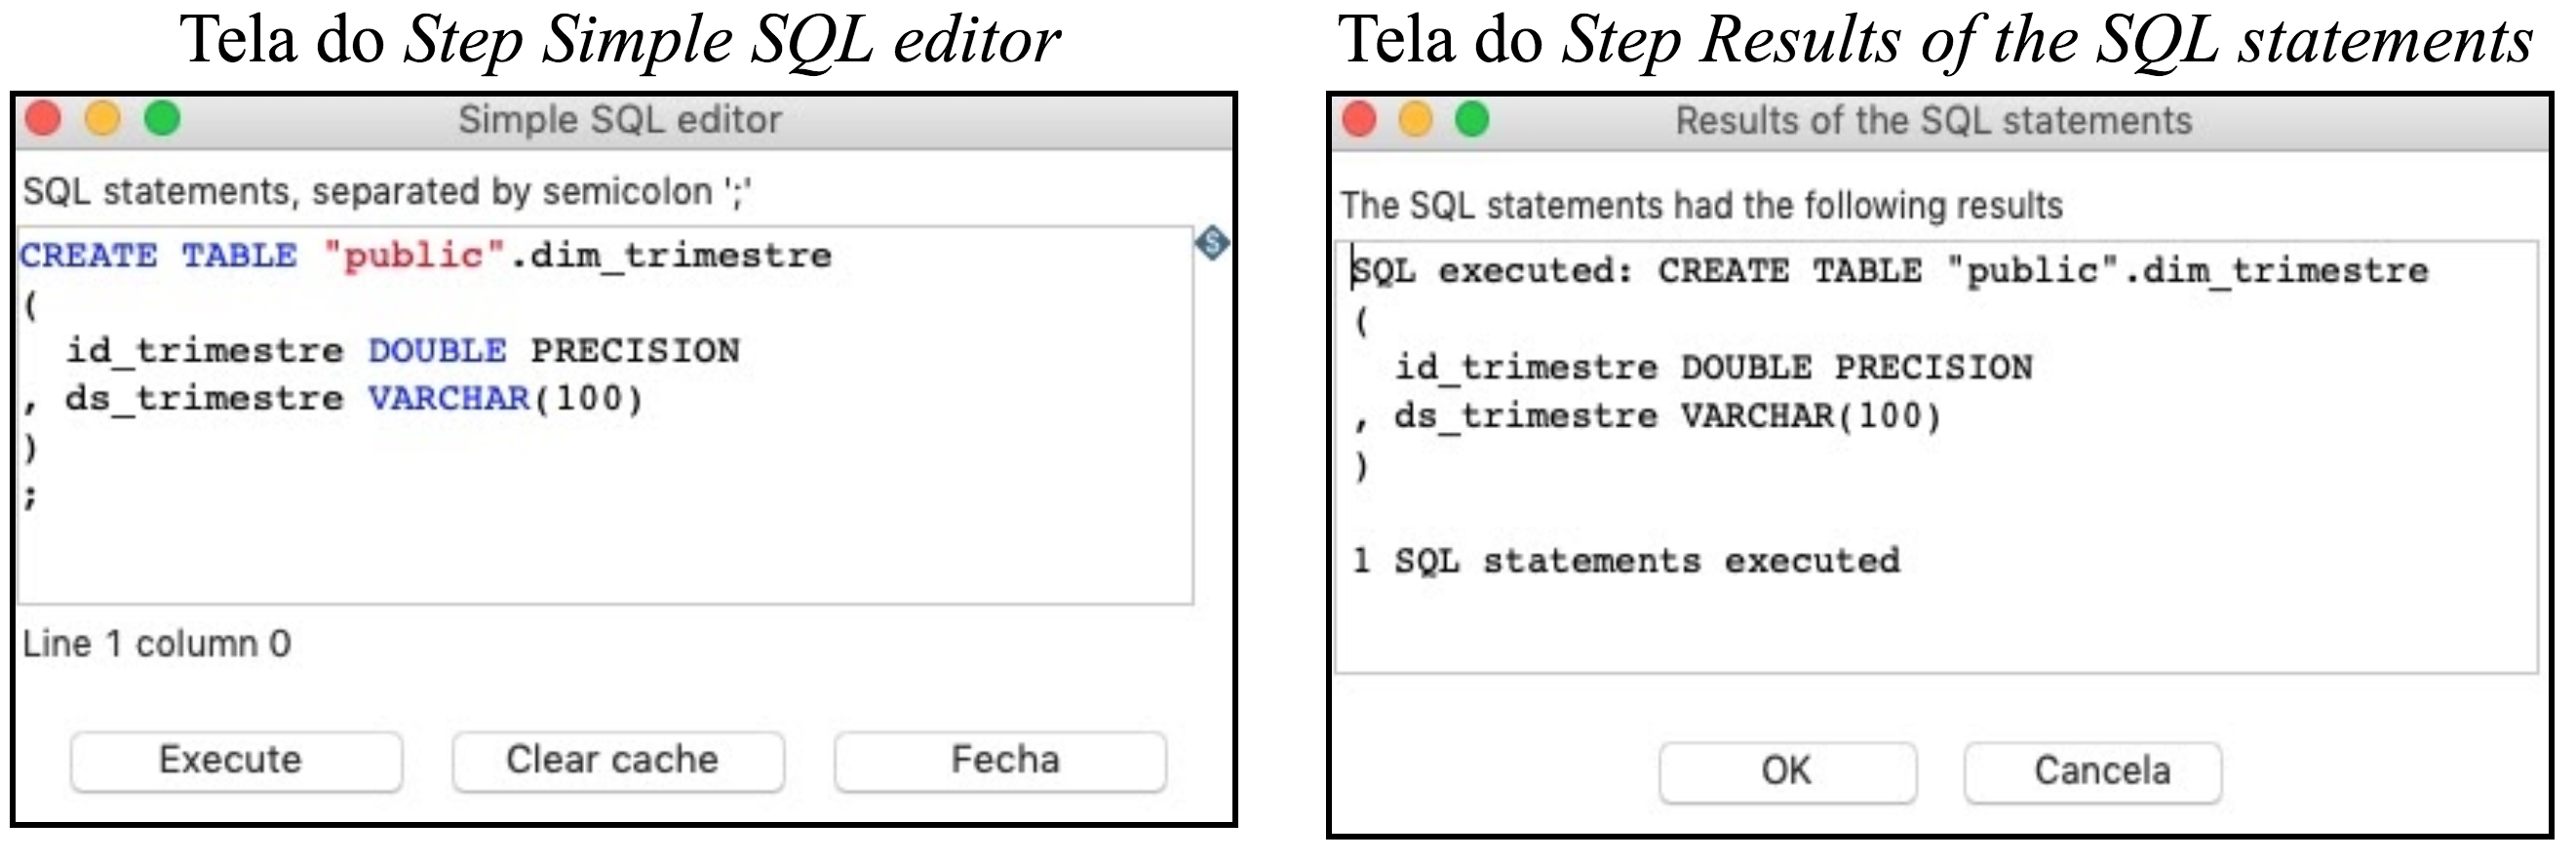
\includegraphics[width=0.6\textwidth]{./04-figuras/figura-tb-dim-trimestre}
    \label{fig:ilustfigtbdimtrimestre}
\end{figure}
\vspace*{-0,9cm}
{\raggedright \fonte{Autor desta monografia, 2020.}} \\

% dim\_semestre
\begin{figure}[H]
	\vspace*{0,2cm}
    \centering
    \caption{Criando a tabela ``dim\_semestre`` atrav\'{e}s da Transforma\c{c}\~{a}o ``dim\_data.ktr''}
    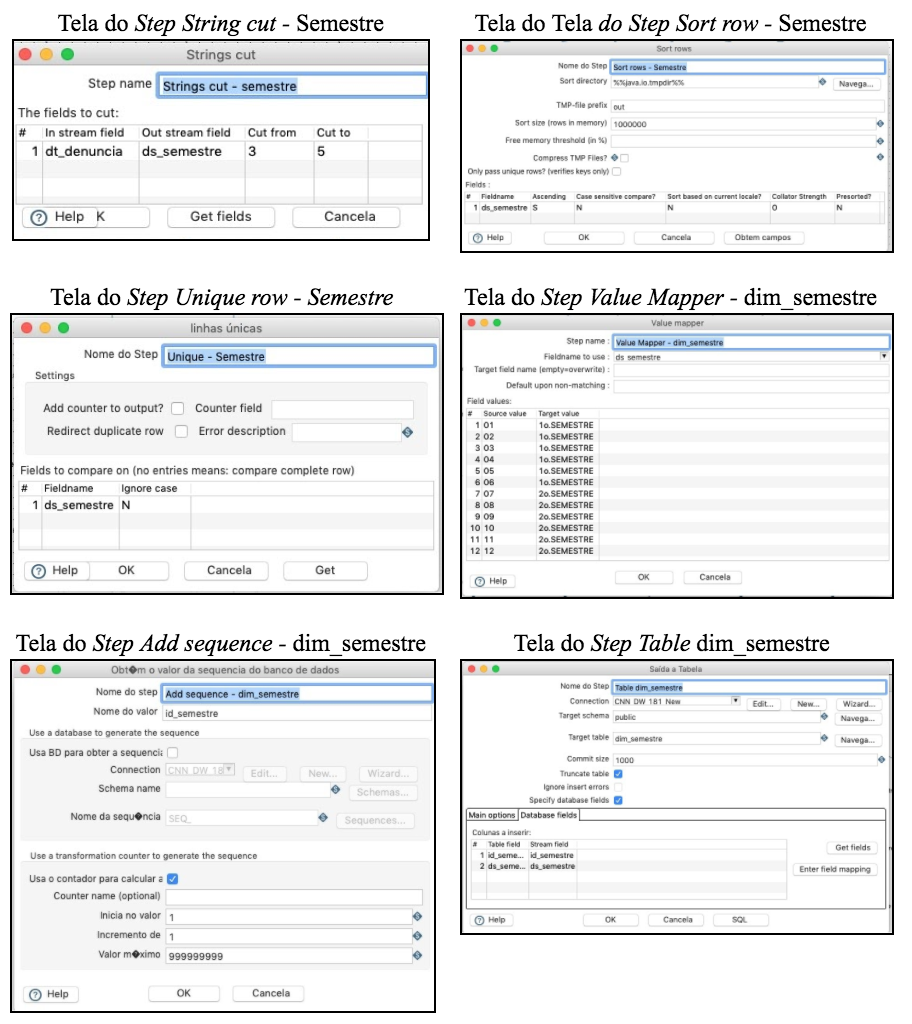
\includegraphics[width=0.6\textwidth]{./04-figuras/figura-dim-semestre}
    \label{fig:ilustfigdimsemestre}
\end{figure}
\vspace*{-0,9cm}
{\raggedright \fonte{Autor desta monografia, 2020.}} \\

\begin{figure}[H]
	\vspace*{0,2cm}
    \centering
    \caption{Criando a tabela ``dim\_semestre`` no banco de dados usando o \textit{step Table} dim\_semestre}
    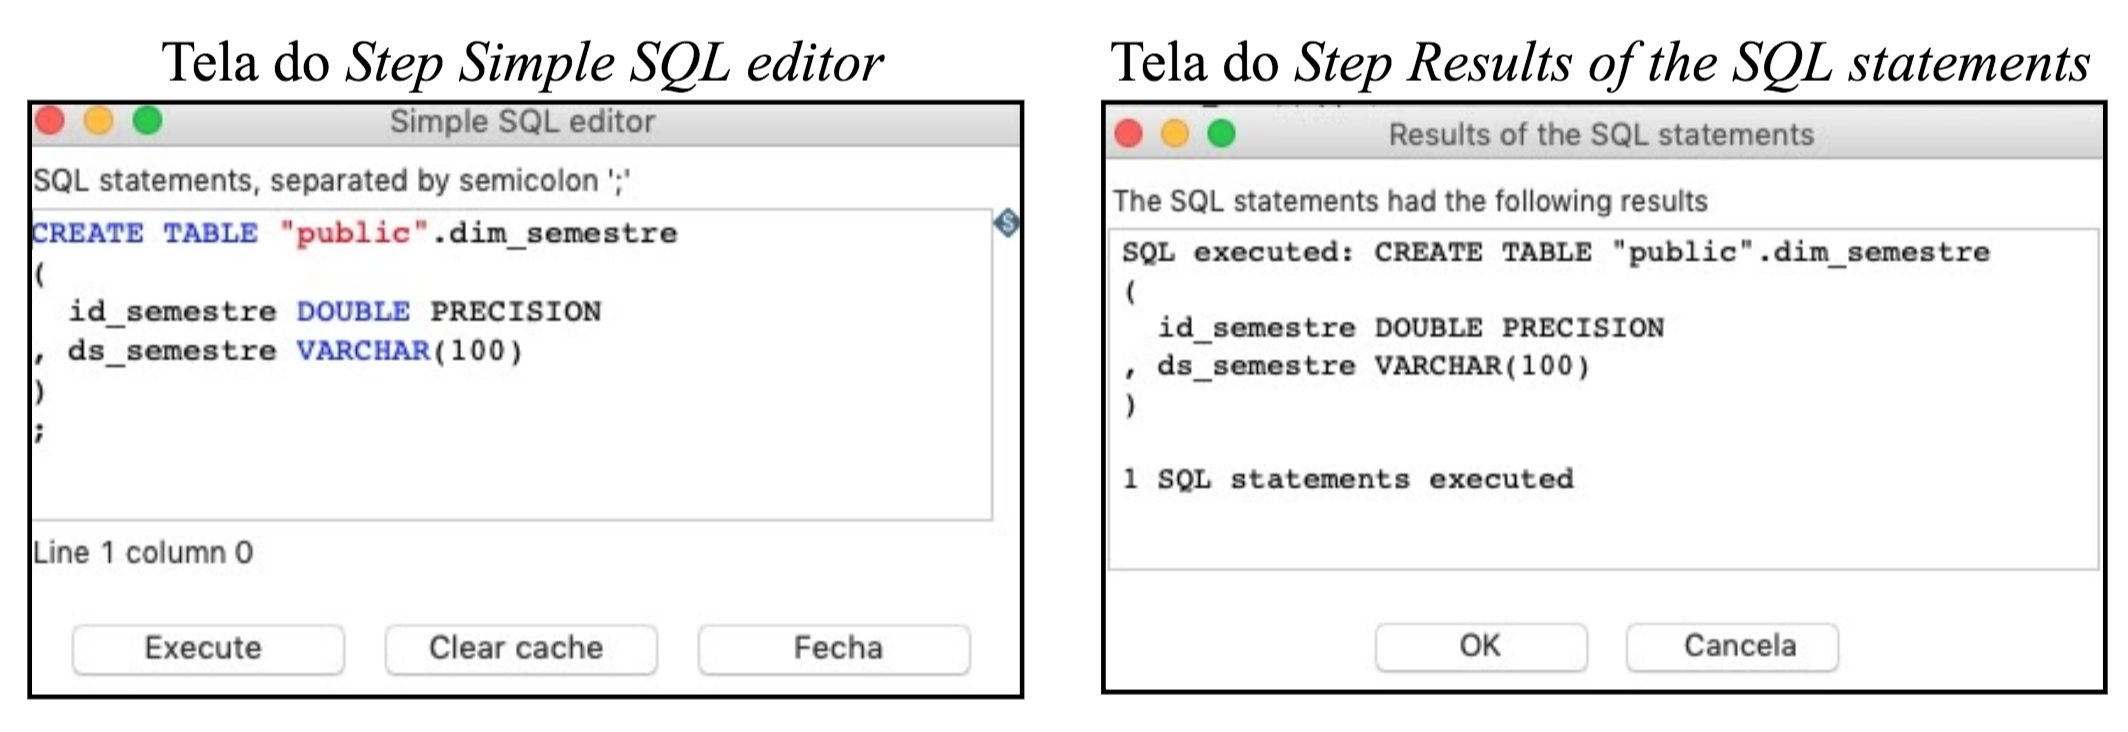
\includegraphics[width=0.6\textwidth]{./04-figuras/figura-tb-dim-semestre}
    \label{fig:ilustfigtbdimsemestre}
\end{figure}
\vspace*{-0,9cm}
{\raggedright \fonte{Autor desta monografia, 2020.}} \\

% dim\_ano
\begin{figure}[H]
	\vspace*{0,2cm}
    \centering
    \caption{Criando a tabela ``dim\_ano'' atrav\'{e}s da Transforma\c{c}\~{a}o ``dim\_data.ktr''}
    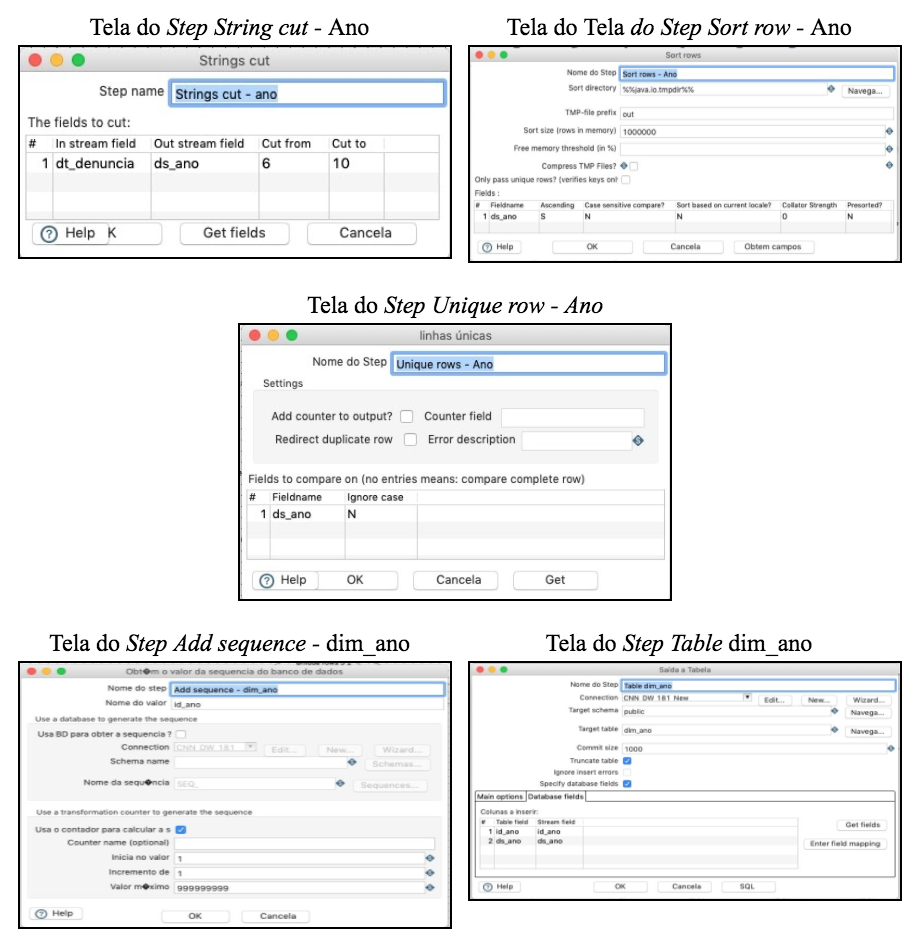
\includegraphics[width=0.6\textwidth]{./04-figuras/figura-dim-ano}
    \label{fig:ilustfigdimano}
\end{figure}
\vspace*{-0,9cm}
{\raggedright \fonte{Autor desta monografia, 2020.}} \\

\begin{figure}[H]
	\vspace*{0,2cm}
    \centering
    \caption{Criando a tabela ``dim\_ano'' no banco de dados usando o \textit{step Table} dim\_ano}
    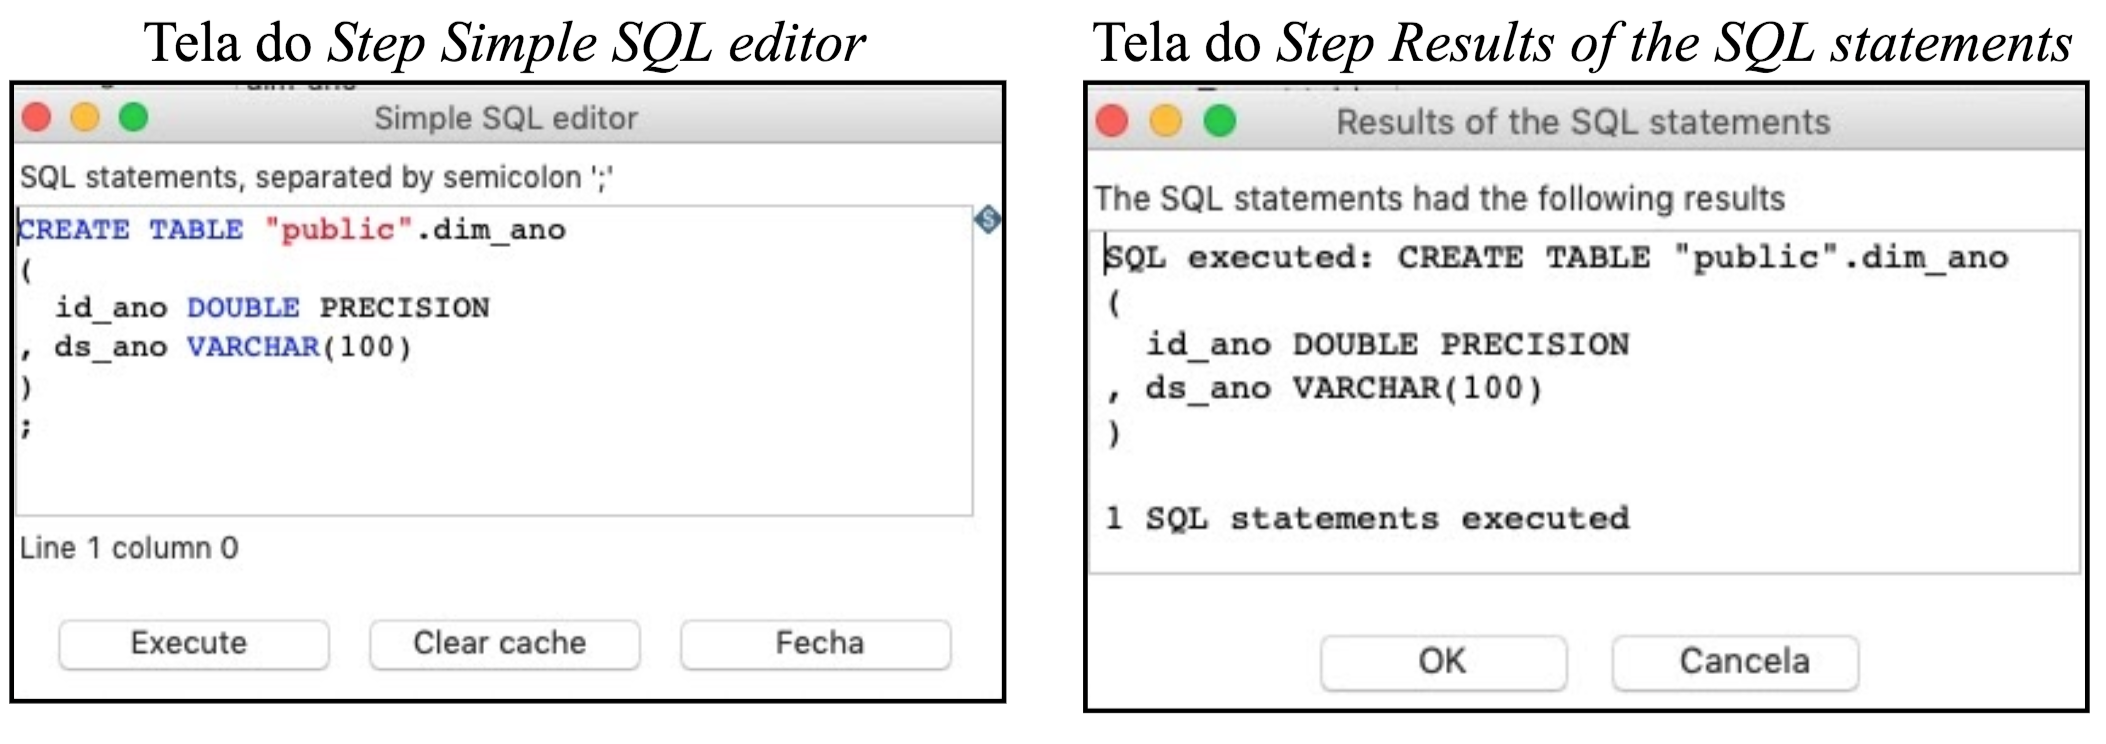
\includegraphics[width=0.6\textwidth]{./04-figuras/figura-tb-dim-ano}
    \label{fig:ilustfigtbdimano}
\end{figure}
\vspace*{-0,9cm}
{\raggedright \fonte{Autor desta monografia, 2020.}} \\

Ao final dos processos quando executamos a transforma\c{c}\~{a}o, conforme figura abaixo, na se\c{c}\~{a}o posterior da tela do PDI, 
em ``Execution Results``. aparecer\'{a} na aba ``Preview data'', os dados padronizados dos campos: 
``dt\_denuncia'', ``ds\_dia''e ``id\_dia''. O pr\'{o}ximo passo ser\'{a} percorrer a grade com os resultado e 
perceber se o processo de transforma\c{c}\~{a}o e carga sai conforme planejado para todas as transforma\c{c}\~{o}es. 

\begin{figure}[H]
	\vspace*{0,2cm}
    \centering
    \caption{Executando a transforma\c{c}\~{a}o ``dim\_data.ktr''}
    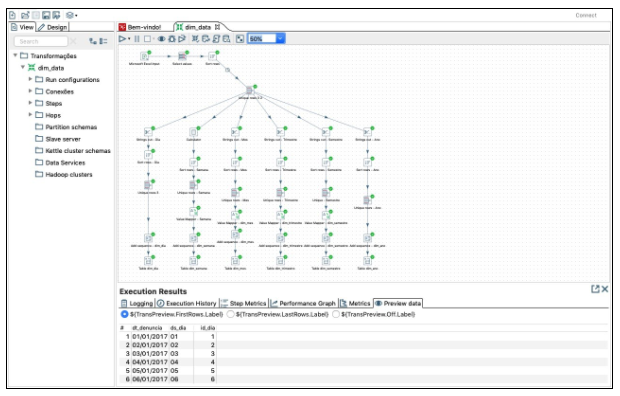
\includegraphics[width=0.6\textwidth]{./04-figuras/figura-exec-dim-data}
    \label{fig:ilustfigtbdimano}
\end{figure}
\vspace*{-0,9cm}
{\raggedright \fonte{Autor desta monografia, 2020.}} \\

Para se ter certeza de que as tabelas: 
``dim\_dia dim\_semana, dim\_mes, dim\_trimestre, dim\_semestre e dim\_ano'', obteve a ETL corretas, 
precisamos abrir as tabelas acima citada no aplicativo pgAdmin4, conforme figura abaixo.

\begin{figure}[H]
	\vspace*{0,2cm}
    \centering
    \caption{Resultado da transforma\c{c}\~{a}o e carga no Banco de Dados ``DW\_181'' na tabela ``dim\_ano''}
    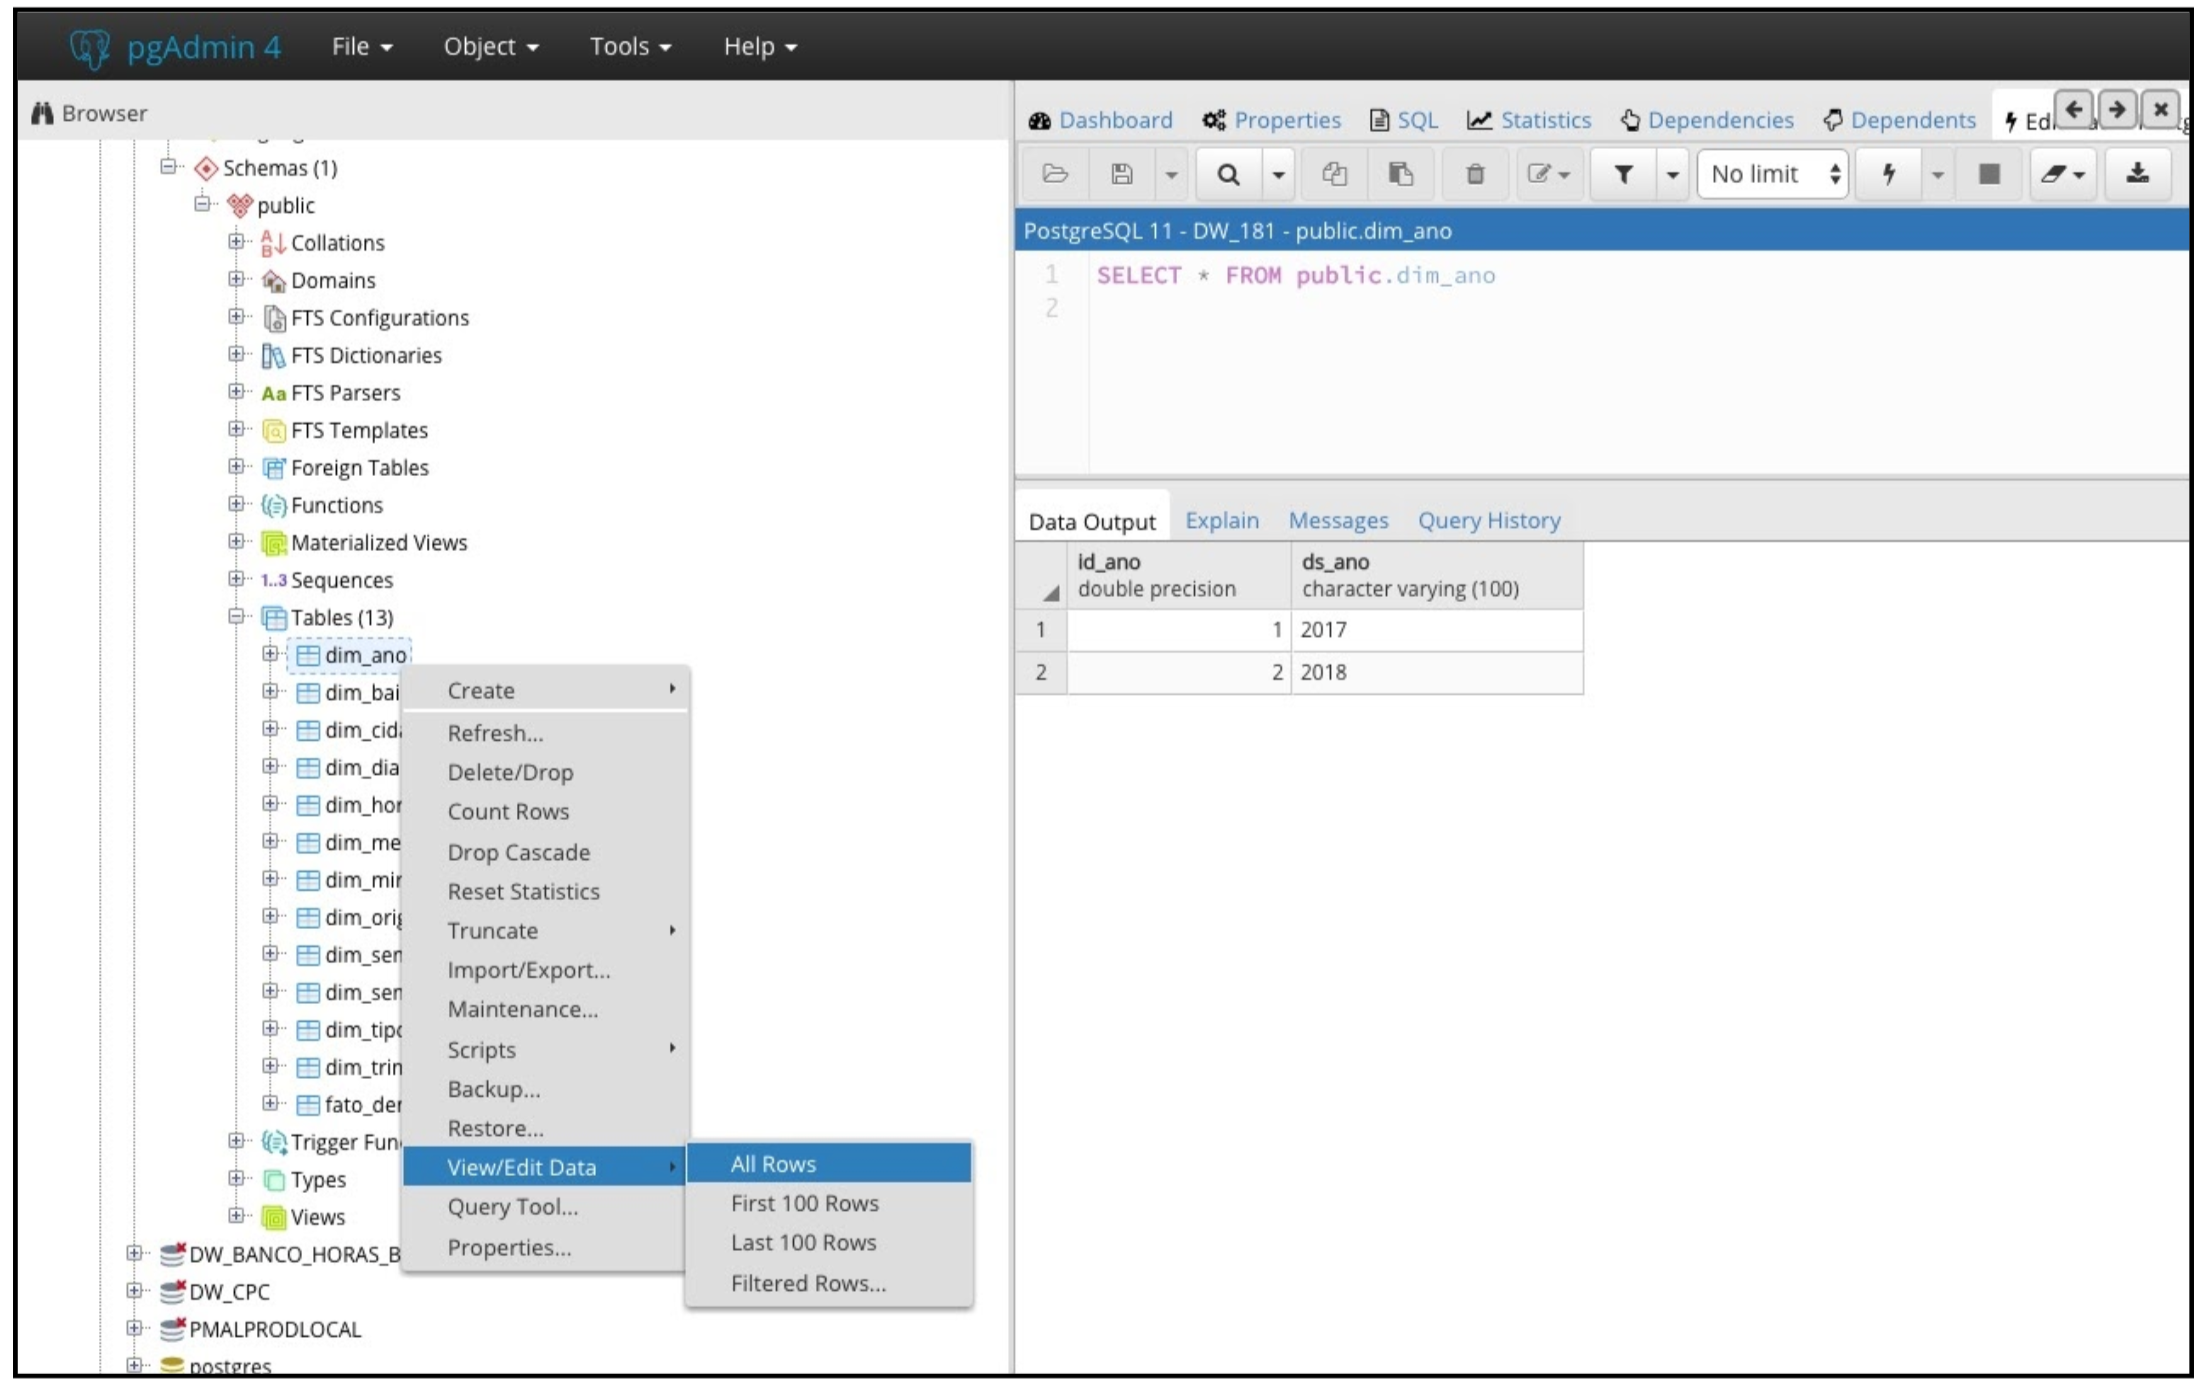
\includegraphics[width=0.6\textwidth]{./04-figuras/figura-res-dim-ano}
    \label{fig:ilustfigresdimano}
\end{figure}
\vspace*{-0,9cm}
{\raggedright \fonte{Autor desta monografia, 2020.}} \\

% TRANSFORMA\C{C}\~{A}O: DIM\_HORA
\subsubsection{Criando a transforma\c{c}\~{a}o ``dim\_hora.ktr''}

A transforma\c{c}\~{a}o ``dim\_hora.ktr'', \'{e} um pouco semelhante a transforma\c{c}\~{a}o ``dim\_data.ktr'', por\'{e}m menos complexa, 
nela iremos usar o \textit{step String cut}, nesta n\~{a}o houve a necessidade do uso de componentes como o \textit{Calculator}. 

O único detalhe \'{e} a movimenta\c{c}\~{a}o dos dados entre o \textit{step Sort rows} para o \textit{Unique rows}, principais, 
que \'{e} : ``Copiar dados para os pr\'{o}ximos steps''. Na figura abaixo, podemos perceber que esta transforma\c{c}\~{a}o tem como 
prioridade criar as tabelas ``dim\_hora'' e a ``dim\_minuto'', ao final de todo processo. 

Assim, iremos produzir dentro do ``DW\_181'', duas novas dimens\~{o}es para que possamos criar an\'{a}lises que podem usar estas dimens\~{o}es.
Iremos, passo a passo e atrav\'{e}s de figuras construir a ETL da transforma\c{c}\~{a}o ``dim\_hora.ktr''.

\begin{figure}[H]
	\vspace*{0,2cm}
    \centering
    \caption{Transforma\c{c}\~{a}o (dim\_hora.ktr) do BI 181}
    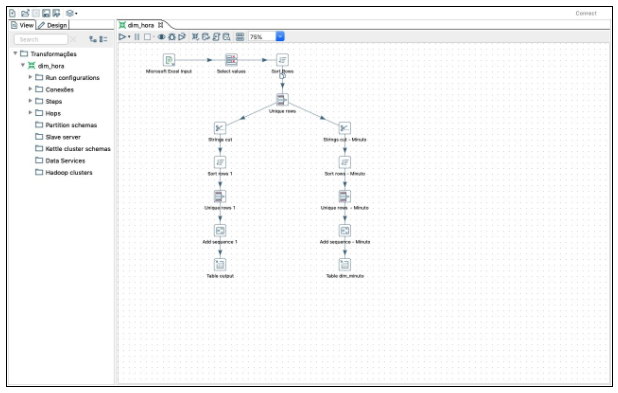
\includegraphics[width=0.6\textwidth]{./04-figuras/figura-dim-hora}
    \label{fig:ilustfigresdimhora}
\end{figure}
\vspace*{-0,9cm}
{\raggedright \fonte{Autor desta monografia, 2020.}} \\

Dividimos a transforma\c{c}\~{o}es em três caminhos, um caminho como sendo o principal que parte do \textit{
step Microsoft Excel Input} at\'{e} o componente Unique rows e dois caminhos que  levam a cria\c{c}\~{a}o das tabelas de cada 
dimens\~{a}o: ``dim\_hora'' e ``dim\_minuto'', conforme as figura acima.

A figura logo abaixo, demonstra a configura\c{c}\~{a}o dos steps do caminho principais.

\begin{figure}[H]
	\vspace*{0,2cm}
    \centering
    \caption{Configurando os \textit{steps} da Transforma\c{c}\~{a}o ``dim\_hora.ktr'' (passo-a-passo)}
    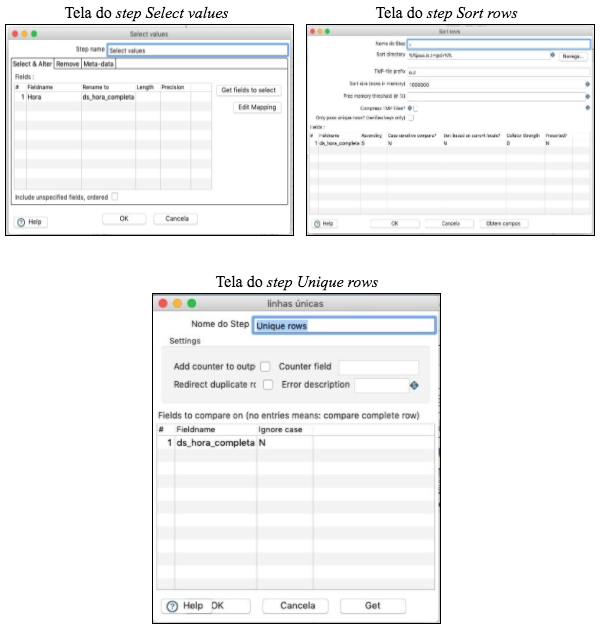
\includegraphics[width=0.6\textwidth]{./04-figuras/figura-dim-hora-passo-a-passo}
    \label{fig:ilustfigdimhorapassoapasso}
\end{figure}
\vspace*{-0,9cm}
{\raggedright \fonte{Autor desta monografia, 2020.}} \\

Como comentado anteriormente, dividimos em dois caminhos, um deles \'{e} formado pelos steps da figura abaixo, 
que representa os componentes que ap\'{o}s execu\c{c}\~{a}o criar\'{a} a tabela ``dim\_hora'' dentro do ``DW\_181''.

\begin{figure}[H]
	\vspace*{0,2cm}
    \centering
    \caption{Criando a tabela ``dim\_hora'' atrav\'{e}s da Transforma\c{c}\~{a}o ``dim\_hora.ktr''}
    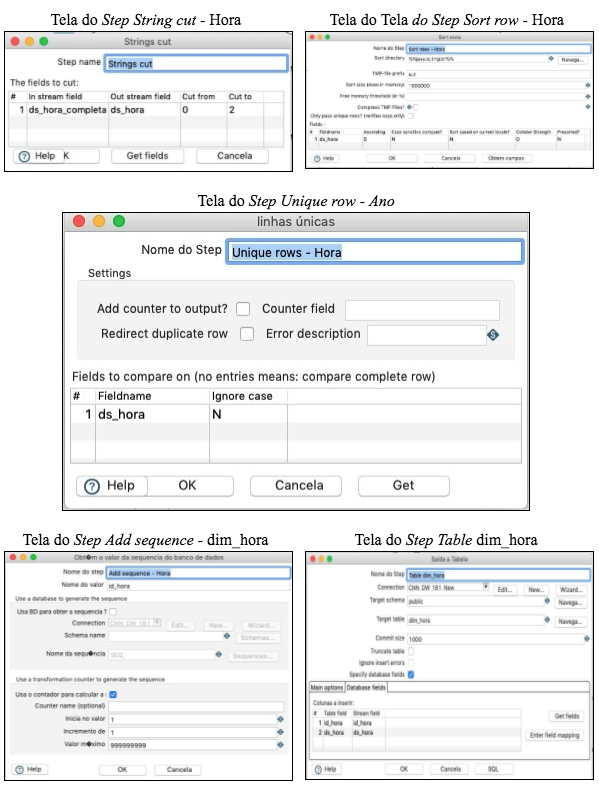
\includegraphics[width=0.6\textwidth]{./04-figuras/figura-trans-dim-hora}
    \label{fig:ilustfigtbdimhora}
\end{figure}
\vspace*{-0,9cm}
{\raggedright \fonte{Autor desta monografia, 2020.}} \\

Quando configuramos devidamente o \textit{step Table} dim\_hora, acessando o bot\~{a}o ``SQL'' na tela do step, 
a figura 74 aparecer\'{a} a tela do \textit{Simple SQL editor}, e ap\'{o}s, acesso ao bot\~{a}o \textit{execute} desta tela,
aparece a tela do \textit{Results of the SQL statements} nos revela o resultado da 
cria\c{c}\~{a}o f\'{i}sica da tabela ``dim\_hora'' dentro do SGDB. 

\begin{figure}[H]
	\vspace*{0,2cm}
    \centering
    \caption{Criando a tabela ``dim\_hora'' no banco de dados usando o \textit{step Table} dim\_hora.}
    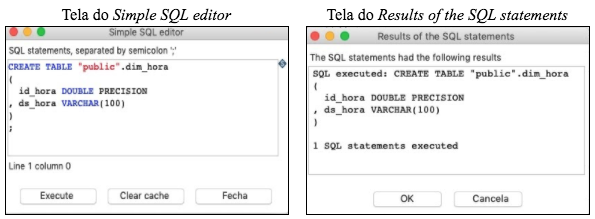
\includegraphics[width=0.6\textwidth]{./04-figuras/figura-tb-dim-hora}
    \label{fig:ilustfigtbdimhora}
\end{figure}
\vspace*{-0,9cm}
{\raggedright \fonte{Autor desta monografia, 2020.}} \\

% dim\_minuto
O outro caminho \'{e} formado pelos \textit{steps} da figura abaixo, que representa os componentes 
que ap\'{o}s execu\c{c}\~{a}o, homologamente ao anterior, criar\'{a} a tabela ``dim\_minuto'' dentro do DW.

\begin{figure}[H]
	\vspace*{0,2cm}
    \centering
    \caption{Criando a tabela ``dim\_minuto'' atrav\'{e}s da Transforma\c{c}\~{a}o ``dim\_data.ktr''}
    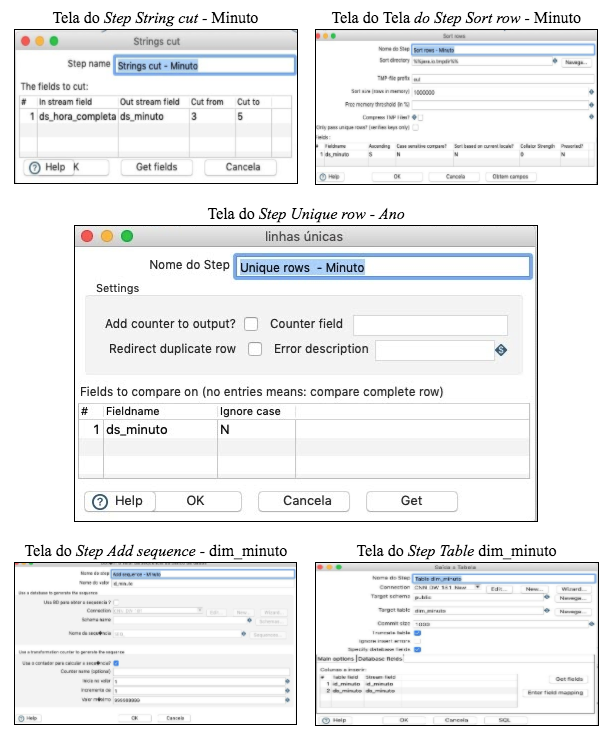
\includegraphics[width=0.6\textwidth]{./04-figuras/figura-dim-minuto}
    \label{fig:ilustfigdimanodimminuto}
\end{figure}
\vspace*{-0,9cm}
{\raggedright \fonte{Autor desta monografia, 2020.}} \\

Tendo como base a configura\c{c}\~{a}o do \textit{step Table} dim\_hora, configuramos o \textit{step Table} dim\_minuto, 
acessando o bot\~{a}o ``SQL'' na tela do \textit{step}, a figura abaixo, na sequência aparecer\'{a} a tela do \textit{Simple 
SQL editor}, e ap\'{o}s, acesso ao bot\~{a}o execute desta tela, a tela do \textit{Results of the SQL statements} 
nos mostra o resultado da cria\c{c}\~{a}o da tabela f\'{i}sica ``dim\_hora'' dentro do SGDB. 

\begin{figure}[H]
	\vspace*{0,2cm}
    \centering
    \caption{Criando a tabela ``dim\_minuto'' no banco de dados usando o \textit{step Table} dim\_minuto}
    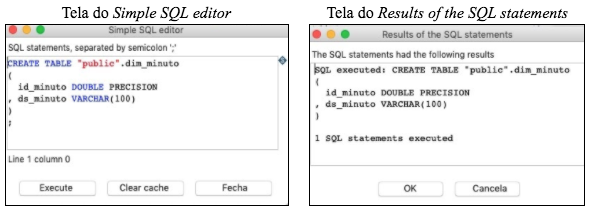
\includegraphics[width=0.6\textwidth]{./04-figuras/figura-tb-dim-minuto}
    \label{fig:ilustfigtbdimminuto}
\end{figure}
\vspace*{-0,9cm}
{\raggedright \fonte{Autor desta monografia, 2020.}} \\

E finalmente, executando a transforma\c{c}\~{a}o ``dim\_hora.ktr'', o resultado do 
processo aparecer\'{a} no quadro ``Execution Results'' da figura seguinte.

\begin{figure}[H]
	\vspace*{0,2cm}
    \centering
    \caption{Executando a transforma\c{c}\~{a}o ``dim\_hora.ktr''}
    \includegraphics[width=0.6\textwidth]{./04-figuras/figura-exec-dim-hora}
    \label{fig:ilustfigexecdimhora}
\end{figure}
\vspace*{-0,9cm}
{\raggedright \fonte{Autor desta monografia, 2020.}} \\

Para se ter certeza de que as tabelas ``dim\_hora'' e ``dim\_minuto'', obtiveram a ETL correta. Para isso como nos t\'{o}picos anteriores 
precisamos abrir a tabela ``dim\_hora'' ou a tabela ``dim\_minuto'' no aplicativo pgAdmin4, do SGDB PostgreSQL, conforme 
as proximas figuras, nelas podemos analisar os dados processados pela transforma\c{c}\~{a}o criada no PDI, ``dim\_hora.ktr'' 
que gerou duas dimens\~{o}es com os dados padronizados inseridos nelas.

\begin{figure}[H]
	\vspace*{0,2cm}
    \centering
    \caption{Resultado da transforma\c{c}\~{a}o e carga no Banco de Dados ``DW\_181'' na tabela ``dim\_hora''}
    \includegraphics[width=0.6\textwidth]{./04-figuras/figura-res-dim-hora}
    \label{fig:ilustfigresdimhora}
\end{figure}
\vspace*{-0,9cm}
{\raggedright \fonte{Autor desta monografia, 2020.}} \\

\begin{figure}[H]
	\vspace*{0,2cm}
    \centering
    \caption{ Resultado da transforma\c{c}\~{a}o e carga no Banco de Dados ``DW\_181'' na tabela ``dim\_minuto''.}
    \includegraphics[width=0.6\textwidth]{./04-figuras/figura-res-dim-minuto}
    \label{fig:ilustfigresdimminuto}
\end{figure}
\vspace*{-0,9cm}
{\raggedright \fonte{Autor desta monografia, 2020.}} \\

% TRANSFORMA\C{C}\~{A}O: FATO\_DEN\]'{U}CIA
\subsubsection{Criando a transforma\c{c}\~{a}o ``fato\_denuncia.ktr''}

Ap\'os criarmos todas as transforma\c{c}\~{o}es nos t\'opicos anteriores,
 precisamos criar a transforma\c{c}\~{a}o que criar\'{a} a tabela fato\_denuncia, 
 que ser\'{a} o centro do modelo estrela segundo Machado (2000), conectada com as dimens\~{o}es j\'{a} 
 criadas nas transforma\c{c}\~{o}es dos t\'opicos anteriores.

Na figura abaixo, podemos destacar o uso de um componente novo no contexto desse trabalho, \'{e} o 
\textit{step Database lookup}, os outros componentes j\'{a} foram usando em t\'opicos anteriores.

\begin{figure}[H]
	\vspace*{0,2cm}
    \centering
    \caption{A transforma\c{c}\~{a}o ``fato\_denuncia.ktr''}
    \includegraphics[width=0.6\textwidth]{./04-figuras/figura-fato}
    \label{fig:ilustfigfato}
\end{figure}
\vspace*{-0,9cm}
{\raggedright \fonte{Autor desta monografia, 2020.}} \\

O uso de componente \textit{Database lookup}, \'{e} o detalhe mais importante para que a transforma\c{c}\~{a}o 
``fato\_denuncia,ktr'', posso atingir o objetivo principal que \'{e} inserir os dados corretos dentro da tabela 
``fato\_denuncia'' dentro do ``DW\_181''. 

O mesmo, precisar ser configurado conforme a abaixo, no campo \textit{connection}, devemos inserir o 
nome da conex\~{a}o com o SGDB, no campo tabela \textit{Lookup}. Logo ap\'{o}s determinar a tabela que servir\'{a} de 
pesquisa no \textit{grid}.

A chave para examinar o valor: devemos inserir os campos de compara\c{c}\~{a}o na 
figura abaixo, a compara\c{c}\~{a}o ficou por conta dos campos: ``ds\_dia''  da tabela de pesquisa, na campo do 
\textit{Grid} ``Campo da tabela'', no campo ``Comparador'', escolhemos a op\c{c}\~{a}o de ``='', e no 
``Campo1'', colocamos o campo provindo e configurado no \textit{step Select values}. Quando a compara\c{c}\~{a}o 
entre os campos \'{e} verificada e encontrada o step retorna o valor configurado no \textit{Grid} Valores a serem 
retornados da tabela \textit{lookup}, que est\'{a} no campo ``campo'' do \textit{Grid} acima, conforme figura abaixo.

\begin{figure}[H]
	\vspace*{0,2cm}
    \centering
    \caption{Componente de \textit{Grid step Database Lookup} - ``dim\_dia''}
    \includegraphics[width=0.6\textwidth]{./04-figuras/figura-step-dl-dim-dia}
    \label{fig:ilustfigstepdldimdia}
\end{figure}
\vspace*{-0,9cm}
{\raggedright \fonte{Autor desta monografia, 2020.}} \\

Outra caracter\'{i}stica da transforma\c{c}\~{a}o ``fato\_denuncia.ktr'' \'{e} o uso do \textit{step Calculator}, como no 
t\'{o}pico ``Criando a transforma\c{c}\~{a}o ``dim\_data.ktr'' '' e  de dois componentes de \textit{step Select values}, o primeiro com os 
campos do arquivo do ``181.xls'' no formato do \textit{Microsoft Excel} e o outro que ap\'{o}s passar por v\'{a}rios \textit{steps} possui 
os futuros campos da tabela de fato ``fato\_denuncia'' que ser\'{a} criada e receber\'{a} os dados conforme o processo de ETL configurado nesta transforma\c{c}\~{a}o.

\begin{figure}[H]
	\vspace*{0,2cm}
    \centering
    \caption{\textit{Step Select values} - fato\_denuncia}
    \includegraphics[width=0.6\textwidth]{./04-figuras/figura-step-sv-fato-denuncia}
    \label{fig:ilustfigstepsvfatodenuncia}
\end{figure}
\vspace*{-0,9cm}
{\raggedright \fonte{Autor desta monografia, 2020.}} \\

\begin{figure}[H]
	\vspace*{0,2cm}
    \centering
    \caption{\textit{Step Table output} - fato\_denuncia}
    \includegraphics[width=0.6\textwidth]{./04-figuras/figura-step-to-fato-denuncia}
    \label{fig:ilustfigsteptofatodenuncia}
\end{figure}
\vspace*{-0,9cm}
{\raggedright \fonte{Autor desta monografia, 2020.}} \\

Depois da configura\c{c}\~{a}o do \textit{step Table output} - fato\_denuncia, clicando no bot\~{a}o ``SQL'' na tela do \textit{step}, 
da figura abaixo, na sequência aparecer\'{a} a tela do \textit{Simple SQL editor}, e ap\'{o}s, um clique no bot\~{a}o ``execute'' 
desta tela, a tela do \textit{Results of the SQL statements} apresenta o resultado da cria\c{c}\~{a}o f\\'{i}{i}sica da tabela 
``fato\_denuncia'' dentro do ``DW\_181'' no Postgres. 

\begin{figure}[H]
	\vspace*{0,2cm}
    \centering
    \caption{Criando a tabela ``fato\_denuncia'' no banco de dados usando o \textit{step Table output}}
    \includegraphics[width=0.6\textwidth]{./04-figuras/figura-tb-fato-denuncia}
    \label{fig:ilustfigtbfatodenuncia}
\end{figure}
\vspace*{-0,9cm}
{\raggedright \fonte{Autor desta monografia, 2020.}} \\

Ao ser executada a transforma\c{c}\~{a}o ``fato\_denuncia.ktr'', o resultado do 
processo aparecer\'{a} no quadro ``Execution Results`` da figura abaixo.

\begin{figure}[H]
	\vspace*{0,2cm}
    \centering
    \caption{Executando a transforma\c{c}\~{a}o ``fato\_denuncia.ktr''}
    \includegraphics[width=0.6\textwidth]{./04-figuras/figura-trans-fato-denuncia}
    \label{fig:ilustfigtransfatodenuncia}
\end{figure}
\vspace*{-0,9cm}
{\raggedright \fonte{Autor desta monografia, 2020.}} \\

O resultado final da transforma\c{c}\~{a}o ``fato\_denuncia.ktr'', ap\'{o}s ser executada \'{e} apresentada na figura 85, 
abaixo, \'{e} percebermos os campos da tabela ``fato\_denuncia'', com os c\'{o}digos de cada tabela de dimens\~{a}o.
Assim, o objetivo desta transforma\c{c}\~{o}es foi alcan\c{c}ado.

\begin{figure}[H]
	\vspace*{0,2cm}
    \centering
    \caption{Resultado da transforma\c{c}\~{a}o e carga no Banco de Dados ``DW\_181'' na tabela fato\_denuncia}
    \includegraphics[width=0.6\textwidth]{./04-figuras/figura-res-fato-denuncia}
    \label{fig:ilustfigresfatodenuncia}
\end{figure}
\vspace*{-0,9cm}
{\raggedright \fonte{Autor desta monografia, 2020.}} \\

% JOBS
\subsubsection{Criando o \textit{JOB} (job\_denuncia)}

Ap\'os termos todas as transforma\c{c}\~{o}es serem criadas e devidamente testadas, faz-se necess\'{a}rio unir 
todas as transforma\c{c}\~{o}es das dimens\~{o}es e a do fato em processo o ``Job'' e nomeado como: ``job\_denuncia.kjb''. 

A \textit{priori} inserimos o componente \textit{start} e logo ap\'os cada transforma\c{c}\~{a}o lembrando que o último 
ser\'{a} o (\textit{Transformation} - fato-denuncia) conforme \`{a} figura abaixo.

\begin{figure}[H]
	\vspace*{0,2cm}
    \centering
    \caption{\textit{Jobs} ``job\_denuncia.kjb'' do BI 181}
    \includegraphics[width=0.6\textwidth]{./04-figuras/figura-job-denuncia}
    \label{fig:ilustfigjobdenuncia}
\end{figure}
\vspace*{-0,9cm}
{\raggedright \fonte{Autor desta monografia, 2020.}} \\

Quando executamos o ``job\_denuncia.kjb'', o resultado aparece na tela inferior a \textit{Execution Results} se a execu\c{c}\~{a}o 
for bem sucedida em cada componente \textit{Transformation} o  componente \textit{Success} aparecer\'{a} conforme a 
figura abaixo ``Sucesso na execu\c{c}\~{a}o'', abaixo em caso contr\'{a}rio o fluxo ser\'{a} desviado para o 
componente \textit{Mail} e o componente que obteve o erro ter\'{a} a apar\^{e}ncia do figura ``Erro na execu\c{c}\~{a}o de 
alguma transforma\c{c}\~{a}o''.

\begin{figure}[H]
	\vspace*{0,2cm}
    \centering
    \caption{\textit{Jobs}  ``job\_denuncia.kjb'' do BI 181 com erro}
    \includegraphics[width=0.6\textwidth]{./04-figuras/figura-job-denuncia-erro}
    \label{fig:ilustfigjobdenunciaerro}
\end{figure}
\vspace*{-0,9cm}
{\raggedright \fonte{Autor desta monografia, 2020.}} \\


Quando executamos o ``job\_denuncia.kjb'' \'{e} o mesmo n\~{a}o tem nenhum erro no fluxo das transforma\c{c}\~{o}es, 
este job se apresentar\'{a} conforme a figura logo abaixo:

\begin{figure}[H]
	\vspace*{0,2cm}
    \centering
    \caption{Executando o \textit{Jobs} ``job\_denuncia.kjb'' do BI 181 no \textit{Spoon}}
    \includegraphics[width=0.6\textwidth]{./04-figuras/figura-exec-job-denuncia}
    \label{fig:ilustfigexecjobdenuncia}
\end{figure}
\vspace*{-0,9cm}
{\raggedright \fonte{Autor desta monografia, 2020.}} \\

Neste t\\'{o}{o}pico finalizamos a fase de ETL usando o PDI, e seus recursos usando os componentes de \textit{Steps, Transformations e Jobs}.

% MODELO DIMENSIONAL
\subsubsection{O modelo dimensional do BI/DW do 181}

Ap\'os a conclus\~{a}o de todas as transforma\c{c}\~{o}es, usando o PDI para desenvolver toda ETL teremos ao final o ``modelo estrela'', 
conforme figura abaixo, com destaque para o conjunto de dimens\~{o}es que comp\~{o}em o tempo (dim\_ano, dim\_mes, dim\_dia, dim\_semana, 
dim\_hora, dim\_minuto, dim\_semestre e a dim\_trimestre) que ser\'{a} essencial quando na fase de anal\'{i}se dos dados usando o \textit{plugin Saiku}. 

Este modelo \'{e} a base de nosso ``DW\_181' e atrav\'{e}s dele nosso BI ser\'{a} 
funcional e poderemos extrair dele as an\'{a}lises que precisaremos para as tomadas de decis\~{o}es.

\begin{figure}[H]
	\vspace*{0,2cm}
    \centering
    \caption{Modelo Dimensional do BI/DW do 181}
    \includegraphics[width=0.6\textwidth]{./04-figuras/figura-moddim}
    \label{fig:ilustfigmoddim}
\end{figure}
\vspace*{-0,9cm}
{\raggedright \fonte{Autor desta monografia, 2020.}} 

% CUBO OLAP
\subsection{Criando o CUBO OLAP}

Em nosso trabalho n\~{a}o iremos nos deter no uso do 
PSW(\textit{Pentaho Schema Workbench} ou Mondrian), apenas iremos demonstrar como 
poderemos criar um cubo usando essa ferramenta que faz parte do pacote do
 Pentaho sem muitos detalhes, pois, podemos criar o cubo dentro do 
 PUC(\textit{Pentaho User Console}), como mostraremos nos pr\'oximos t\'opicos.

\begin{figure}[H]
	\vspace*{0,2cm}
    \centering
    \caption{tela do PSW (\textit{Pentaho Schema Workbench} ou Mondrian)}
    \includegraphics[width=0.6\textwidth]{./04-figuras/figura-pentaho-psw}
    \label{fig:ilustfigpentaho-psw}
\end{figure}
\vspace*{-0,9cm}
{\raggedright \fonte{Autor desta monografia, 2020.}} \\

\begin{figure}[H]
	\vspace*{0,2cm}
    \centering
    \caption{Publicando o CUBO usando o Mondrian}
    \includegraphics[width=0.6\textwidth]{./04-figuras/figura-pentaho-psw-publicando}
    \label{fig:ilustfigpentahopswpublicando}
\end{figure}
\vspace*{-0,9cm}
{\raggedright \fonte{Autor desta monografia, 2020.}} \\

\begin{figure}[H]
	\vspace*{0,2cm}
    \centering
    \caption{CUBO publicado com sucesso}
    \includegraphics[width=0.6\textwidth]{./04-figuras/figura-pentaho-psw-publicado-sucesso}
    \label{fig:ilustfigpentahopswpublicadosucesso}
\end{figure}
\vspace*{-0,9cm}
{\raggedright \fonte{Autor desta monografia, 2020.}} \\

\begin{figure}[H]
	\vspace*{0,2cm}
    \centering
    \caption{PME (\textit{Pentaho Meta Data Editor})}
    \includegraphics[width=0.6\textwidth]{./04-figuras/figura-pentaho-pme}
    \label{fig:ilustfigpentahopentahopme}
\end{figure}
\vspace*{-0,9cm}
{\raggedright \fonte{Autor desta monografia, 2020.}} \\

% PENTAHO
\subsection{Iniciando o servidor Pentaho}

Ap\'os a fase de ETL utilizando o PDI (Pentaho Data Integration), a mesma sendo testada no SGBD Postgres, 
e logo ap\'os a cria\c{c}\~{a}o do cubo atrav\'{e}s do PSW (\textit{Pentaho Schema Workbench}) iremos para a fase de implementa\c{c}\~{a}o do BI com objetivo de usarmos o PUC (\textit{Pentaho User Console}).

Inicialmente executaremos o servidor \textit{Tomcat} conforme a figura abaixo, 
e para isso devemos usar o terminal em linha de comando do Sistema Operacional MacOSX Catalina, e 
nos direcionando via comando do console para a pasta:

``Applications/Pentaho/pentaho-server'' usando o comando ``cd`` e se 
localizar na pasta ``Pentaho-server'', usaremos o comando: ``./start-pentaho.sh``.

\begin{figure}[H]
	\vspace*{0,2cm}
    \centering
    \caption{Comando no Terminal para iniciar o servidor \textit{Tomcat}.}
    \includegraphics[width=0.6\textwidth]{./04-figuras/figura-pserver}
    \label{fig:ilustfigpserver}
\end{figure}
\vspace*{-0,9cm}
{\raggedright \fonte{Autor desta monografia, 2020.}} \\

Ap\'os executarmos o comando do par\'{a}grafo anterior a aparece na tela do console as informa\c{c}\~{o}es de 
conex\~{a}o com o servidor \textit{Tomcat}, conforme figura logo abaixo.

\begin{figure}[H]
	\vspace*{0,2cm}
    \centering
    \caption{Comando no Terminal para iniciar o servidor \textit{Tomcat}.}
    \includegraphics[width=0.6\textwidth]{./04-figuras/figura-pserver-iniciando}
    \label{fig:ilustfigpserveriniciando}
\end{figure}
\vspace*{-0,9cm}
{\raggedright \fonte{Autor desta monografia, 2020.}} \\

Ap\'{o}s os procedimentos e comandos realizados nos par\'{a}grafos acima, devemos acompanhar o pr\'{o}ximo t\'{o}pico 
destinado ao uso do PUC (\textit{Pentaho User Console}).

% PUC
\subsection{Utilizando o PUC (\textit{Pentaho User Console})}

O princ\'{i}pio do uso do \textit{Pentaho User Console} tem a similaridade de quando usamos as 
ferramentas de gerenciamento de arquivos ou qualquer navegador da Web, \'{e} como se estiv\'{e}ssemos 
usando o PUC. \'{e} essa a analogia em rela\c{c}\~{a}o ao Console de Usu\'{a}rios Pentaho (PUC) que 
devemos ter em mente para usar esse console. Assim para se familiarizar com as diferentes p\'{a}ginas e 
controles da PUC, nesse t\'opico iremos detalhar seu uso de uma forma simplificada seguindo o padr\~{a}o do 
manual do Pentaho (2020).

Primeiramente iniciaremos o navegador que pode ser qualquer um, por\'{e}m, em nosso trabalho 
iremos usar o navegador web denominado Safari, que \'{e} o padr\~{a}o dos SOs, iOS e macOSX da Apple, 
e usaremos a URL do servidor Pentaho em nosso trabalho ser\'{a}: ``http://localhost:8080``.  
Ao digitarmos a p\'{a}gina carrega uma tela introdut\'oria com uma se\c{c}\~{a}o de login, como na figura , abaixo.

\begin{figure}[H]
	\vspace*{0,2cm}
    \centering
    \caption{tela do PUC (\textit{Pentaho User Console})}
    \includegraphics[width=0.6\textwidth]{./04-figuras/figura-puc}
    \label{fig:ilustfigpuc}
\end{figure}
\vspace*{-0,9cm}
{\raggedright \fonte{Autor desta monografia, 2020.}} \\

Como padr\~{a}o o console possui a op\c{c}\~{a}o ``Entre como um Avaliador'', que nos fornece as senhas conforme a figura acima.

Ao entramos com o usu\'{a}rio e a senha no PUC podemos escolher os temas pr\'{e}-instalados 
(\textit{Crystal, Ruby e Sapphire}), em nossos exemplos iremos usar o tema \textit{Crystal}, por\'{e}m, o na vers\~{a}o que usamos 
neste trabalho o tema padr\~{a}o \'{e} o \textit{Ruby}, logo abaixo os exemplos dos temas nas figuras.

\begin{figure}[H]
	\vspace*{0,2cm}
    \centering
    \caption{Tela inicial do PUC com o tema \textit{Crystal}}
    \includegraphics[width=0.6\textwidth]{./04-figuras/figura-puc-tema-cristal}
    \label{fig:ilustfiguctemacristal}
\end{figure}
\vspace*{-0,9cm}
{\raggedright \fonte{Autor desta monografia, 2020.}} \\

\begin{figure}[H]
	\vspace*{0,2cm}
    \centering
    \caption{Tela inicial do PUC com o tema \textit{Ruby}}
    \includegraphics[width=0.6\textwidth]{./04-figuras/figura-puc-tema-ruby}
    \label{fig:ilustfigpuctemaruby}
\end{figure}
\vspace*{-0,9cm}
{\raggedright \fonte{Autor desta monografia, 2020.}} \\

\begin{figure}[H]
	\vspace*{0,2cm}
    \centering
    \caption{Tela inicial do PUC com o tema \textit{Sapphyre}}
    \includegraphics[width=0.6\textwidth]{./04-figuras/figura-puc-tema-sapphyre}
    \label{fig:ilustfigpuctemasapphyre}
\end{figure}
\vspace*{-0,9cm}
{\raggedright \fonte{Autor desta monografia, 2020.}} \\

Para que o Console do Usu\'{a}rio tenha a sua funcionalidade melhorada precisamos criar a 
fonte de Dados e nela criar o esquema estrela dentro do PUC. No pr\'{o}ximo t\'{o}pico iremos criar a 
foto de dados para podermos ter acesso às an\'{a}lises que ser\~{a}o implementadas nessa monografia.

% Gerenciando as fontes de dados
\subsubsection{Gerenciando as fontes de dados}

Ao clicarmos com o mouse no bot\~{a}o ``Gerenciar Fonte de Dados'', a tela da figura abaixo, aparece, nela 
temos um grid com as fontes de dados e os tipos j\'{a} definidos ou e no bot\~{a}o ``Nova Origem de Dados'' 
no lado direito superior da janela, ou podemos editar e fazer outras opera\c{c}\~{o}es nas fontes de dados, 
conforme as nossas necessidades usando o \'{i}cone de engrenagem ao lado do bot\~{a}o ``Nova Origem de Dados''.

\begin{figure}[H]
	\vspace*{0,2cm}
    \centering
    \caption{Tela da op\c{c}\~{a}o Gerenciar Fonte de Dados no PUC}
    \includegraphics[width=0.6\textwidth]{./04-figuras/figura-puc-fonte-de-dados}
    \label{fig:ilustfigpucfontededados}
\end{figure}
\vspace*{-0,9cm}
{\raggedright \fonte{Autor desta monografia, 2020.}} \\

Antes de criarmos nossas fontes de dados e an\'{a}lises, teremos que criar uma nova conex\~{a}o 
com o Banco de dados dentro do PUC, e para isso deveremos observar a figura abaixo:

\begin{figure}[H]
	\vspace*{0,2cm}
    \centering
    \caption{Janela da Fonte de Dados na Op\c{c}\~{a}o ``Nova Conex\~{a}o''}
    \includegraphics[width=0.6\textwidth]{./04-figuras/figura-puc-fonte-de-dados-nova-conexao}
    \label{fig:ilustfigppucfontededadosnovaconexao}
\end{figure}
\vspace*{-0,9cm}
{\raggedright \fonte{Autor desta monografia, 2020.}} \\

Ap\'{o}s a sele\c{c}\~{a}o da op\c{c}\~{a}o ``Nova conex\~{a}o'' da janela da figura acima, poderemos configurar essa nova 
conex\~{a}o, conforme a Tela da figura 99, abaixo.

Por padr\~{a}oo usamos o prefixo ``cnn'' ou ``CNN'' para qualquer conex\~{a}o dentro do PUC.

\begin{figure}[H]
	\vspace*{0,2cm}
    \centering
    \caption{Configurando uma nova conex\~{a}o de Banco de Dados no PUC}
    \includegraphics[width=0.6\textwidth]{./04-figuras/figura-puc-conexao-bd}
    \label{fig:ilustfigpucconexaobd}
\end{figure}
\vspace*{-0,9cm}
{\raggedright \fonte{Autor desta monografia, 2020.}} \\

Quando todos os par\^{a}metros da janela de conex\~{a}o com o Banco de Dados estiver configurado, 
podemos fazer o teste na conex\~{a}o, e em caso da conex\~{a}o est\'{a} bem sucedida a janela da figura abaixo, aparece no PUC.

\begin{figure}[H]
	\vspace*{0,2cm}
    \centering
    \caption{Testando a nova conex\~{a}o}
    \includegraphics[width=0.6\textwidth]{./04-figuras/figura-puc-testando-uma-nova-conexao}
    \label{fig:ilustfigppuctestandoumanovaconexao}
\end{figure}
\vspace*{-0,9cm}
{\raggedright \fonte{Autor desta monografia, 2020.}} \\

Com a conex\~{a}o denominada ``CNN\_DW\_181'' configurada e testada, iremos criar a an\'{a}lise 
no pr\'{o}ximo t\'{o}pico, com base no esquema estrela j\'{a} explicado neste trabalho no 
t\'{o}pico de Modelagem multidimensional.

% Esquema estrela CUBO_DW_181
\subsubsection{Criando o esquema estrela no PUC e o CUBO\_DW\_181}

Para criamos a an\'{a}lise precisamos preencher os par\^{a}metros, conforme a figura abaixo, \textit{a priori} digitando 
o nome da fonte de dados que ser\'{a} a base da nossa an\'{a}lise fundamentada em um esquema estrela denominada
``CUBO\_DW_\181'', logo ap\'{o}s nome\'{a}-la, devemos selecionar o Tipo da Fonte como ``Tabela(s) do Banco de Dado(s), 
a conex\~{a}o ``CNN\_DW\_181'', \'{e} a depois de selecionarmos a conex\~{a}o, devemos selecionar a op\c{c}\~{a}o ``Relat\'{o}rio e An\'{a}lises
(Requer um Esquema Estrela)``, esta \'{e} a forma mais simples de criar um esquema estrela, sem o uso do Mondrian. 
Ao final selecionaremos o bot\~{a}o  ``Pr\'{o}ximo >'', e continuar as configura\c{c}\~{a}o das telas que vir\~{a}o.  

\begin{figure}[H]
	\vspace*{0,2cm}
    \centering
    \caption{Utilit\'{a}rio de fonte de Dados (Selecione Tipo)}
    \includegraphics[width=0.6\textwidth]{./04-figuras/figura-puc-utiliario-fonte-de-dados-selecione-tipo}
    \label{fig:ilustfigpucutiliariofontededadosselecionetipo}
\end{figure}
\vspace*{-0,9cm}
{\raggedright \fonte{Autor desta monografia, 2020.}} \\

Depois de toda configura\c{c}\~{a}o da figura acima iremos configurar o esquema estrela a partir das janelas que se seguem nas pr\'{o}ximas figuras.

Na figura abaixo, deveremos selecionar todas as tabelas no quadro das Tabelas Dispon\'{i}veis e enviaremos para o quadro das Tabelas Selecionadas como na 
figura abaixo, e na combo grid Tabela de Fato, deveremos selecionar a tabela ``public``.``fato_denuncia``, para que o bot\~{a}o ``Pr\'{o}ximo >`` possa ser 
selecionado, caso contr\'{a}rio o mesmo fica indispon\'{i}vel e n\~{a}o dar\'{a} acesso a Janela da figura. Como todas as configura\c{c}\~{o}es da janela da 
figura  realizadas precisamos apenas selecionar o bot\~{a}o ``Pr\'{o}ximo >`` para que, possamos continuar a cria\c{c}\~{a}o do an\'{a}lise cujo modelo ser\'{a} 
o estrela onde poderemos us\'{a}-la dentro dos plugins: \textit{Saiku Analytics e o Jpivot Analysis} que foram detalhas nos T\'{o}picos: 4.4.6.3 e 4.4.6.4. 

\begin{figure}[H]
	\vspace*{0,2cm}
    \centering
    \caption{Utilit\'{a}rio de fonte de Dado (Tabelas}
    \includegraphics[width=0.6\textwidth]{./04-figuras/figura-puc-utiliario-fonte-de-dados-tabelas}
    \label{fig:ilustfigpucutiliariofontededadostabelas}
\end{figure}
\vspace*{-0,9cm}
{\raggedright \fonte{Autor desta monografia, 2020.}} \\

Ao finalizarmos o processo de configura\c{c}\~{a}o da Tela da figura, deveremos relacionar as Tabelas da Esquerda, com as Tabelas da Direita, 
sempre pelos campos iniciados com o ``id\_'' de suas respectivas tabelas. Com esse recurso teremos as rela\c{c}\~{o}es entre as Tabela de dimens\~{o}es 
com a Tabela de Fato denominada anteriormente de ``fato_denuncia''. Quando todos os relacionamentos estiverem prontos no campo ``Relacionamento(s)'' 
o bot\~{a}o ``Finalizar'' ficarem dispon\'{i}vel para que finalizarmos o esquema estrela do ``CUBO\_DW\_181``, conforme a Tela da figura que tem os 
par\^{a}metros para a defini\c{c}\~{a}o das rela\c{c}\~{o}es entre as tabelas.

\begin{figure}[H]
	\vspace*{0,2cm}
    \centering
    \caption{Utilit\'{a}rio de fonte de Dados (Definir Rela\c{c}\~{o}es)}
    \includegraphics[width=0.6\textwidth]{./04-figuras/figura-puc-utiliario-fonte-de-dados-relacoes}
    \label{fig:ilustfigpucutiliariofontededadosrelacoes}
\end{figure}
\vspace*{-0,9cm}
{\raggedright \fonte{Autor desta monografia, 2020.}} \\

Quando selecionarmos o bot\~{a}o finalizar da figura, poderemos modelar a fonte de dados 
criada, por\'{e}m, neste trabalho n\~{a}o iremos precisar de tal processo, pois os nomes dos campos 
est\~{a}o bastantes intuitivos e de f\'{a}cil compreens\~{a}o. O importante \'{e} que o PUC, em sua modelagem 
de fonte de dados, conforme a figura abaixo, nos permite personalizar os nomes, tamanhos e etc dos 
campos das tabelas de dimens\~{o}es e a de fato, sem que necessitarmos de uma ferramenta externa como 
o \textit{Mondrian}, facilitando assim o trabalho de um projeto b\'{a}sico de BI usando o Pentaho e o PUC, para 
um DW simples, eficiente e funcional.

Quando terminarmos todas as configura\c{c}\~{o}es contidas nesse T\'{o}pico, relacionadas com a Fonte de dados, 
poderemos us\'{a}-la, dentro de alguns \textit{plugins} disponibilizados dentro do \textit{Marketplace} do Pentaho, principalmente
 no \textit{Saiku Analytics} e o \textit{Jpivot Analysis} que nos ajudaram a dar vaz\~{a}o aos CUBOS, gr\'{a}ficos e tabelas com dados 
 estat\'{i}sticos fundamentos esses do nosso DW.

 \begin{figure}[H]
	\vspace*{0,2cm}
    \centering
    \caption{Fontes de Dados}
    \includegraphics[width=0.6\textwidth]{./04-figuras/figura-puc-modelagem-fonte-de-dados}
    \label{fig:ilustfigpucmodelagemfontededados}
\end{figure}
\vspace*{-0,9cm}
{\raggedright \fonte{Autor desta monografia, 2020.}} \\

Ao final de toda configura\c{c}\~{a}o teremos dispon\'{i}vel a fonte de dados ``CUBO_DW_181``, 
conforme a figura abaixo.

\begin{figure}[H]
	\vspace*{0,2cm}
    \centering
    \caption{Fontes de Dados}
    \includegraphics[width=0.6\textwidth]{./04-figuras/figura-puc-testando-uma-nova-conexao}
    \label{fig:ilustfigpuctestandoumanovaconexao}
\end{figure}
\vspace*{-0,9cm}
{\raggedright \fonte{Autor desta monografia, 2020.}} \\

% Saiku Analytics
\subsubsection{Usando o \textit{Saiku Analytics}}

No cap\'{i}tulo 4 Desenvolvimento, T\'{o}pico 4.3.2.4.1, teorizamos sobre o plugin Saiku Analytics neste, iremos us\'{a}-lo 
para analisar informa\c{c}\~{o}es sobre os dados provenientes da Fonte de Dados ``CUBO\_DW\_181'', criado no t\'{o}pico acima.
Na figura 106, demonstramos as op\c{c}\~{o}es de acesso ao plugin, o mesmo n\~{a}o vem por padr\~{a}o pr\'{e}-instalado dentro do PUC, 
precisamos selecionar o mesmo no Marketplace do Pentaho, esta passo n\~{a}o iremos demonstrar em nosso material. Iremos apenas us\'{a}-lo.
Conforme a figura abaixo, a primeira op\c{c}\~{a}o (Op\c{c}\~{a}o 1 - Acesso pelo Menu do PUC) nos dar acesso ao plugin atrav\'{e}s do menu 
de contexto do PUC a segunda op\c{c}\~{a}o (Op\c{c}\~{a}o 2 - Acesso pelo Bot\~{a}o do PUC) se utiliza dos bot\~{o}es apresentados na tela do PUC.

\begin{figure}[H]
	\vspace*{0,2cm}
    \centering
    \caption{Op\c{c}\~{o}es de acesso ao \textit{Saiku Analytics}}
    \includegraphics[width=0.6\textwidth]{./04-figuras/figura-puc-saiku-opcoes-acesso}
    \label{fig:ilustfigpucsaikuopcoesacesso}
\end{figure}
\vspace*{-0,9cm}
{\raggedright \fonte{Autor desta monografia, 2020.}} \\

Para usarmos o Saiku, precisamos acessar o mesmo ap\'{o}s termos escolhido uma das op\c{c}\~{o}es de acesso da figura 106, acima, 
quando escolhemos uma nova tela aparece e logo abaixo dela h\'{a} a descri\c{c}\~{a}o em inglês do plugin, e depois desta descri\c{c}\~{a}o
 usaremos o menu de bot\~{o}es denominado Quick Links, e selecionaremos o bot\~{a}o ``Create a new query'', conforme a figura 107,  ap\'{o}s 
 acesso a esse bot\~{a}o a tela da figura 108, ser\'{a} apresentada.

\begin{figure}[H]
	\vspace*{0,2cm}
    \centering
    \caption{Op\c{c}\~{o}es do \textit{Saiku Analytics}}
    \includegraphics[width=0.6\textwidth]{./04-figuras/figura-puc-saiku-opcoes}
    \label{fig:ilustfigpucsaikuopcoes}
\end{figure}
\vspace*{-0,9cm}
{\raggedright \fonte{Autor desta monografia, 2020.}} \\

Na figura 108, \'{e} onde h\'{a} a m\'{a}gica se inicia, nela iremos atrav\'{e}s de sele\c{c}\~{a}o do cubo, da configura\c{c}\~{a}o das: medidas e as dimens\~{o}es. 
Para podermos ver os resultados precisamos apenas arrastar e soltar os campos das dimens\~{o}es nos quadros: medidas, colunas, linhas e filtros de acordo com a necessidade 
do analista de dados ou do gestor do BI.

Conforme a figura 108, temos um pool de op\c{c}\~{o}es, para podermos personalizar, os gr\'{a}ficos as formas de demonstrar os dados vindo do CUBO e ao final 
salva a an\'{a}lise para consultas futuras.   
Ser\'{a} nesse ambiente dentro do PUC que iremos trabalhar e criar as nossas an\'{a}lises de acordo com nossas necessidades, fornecendo informa\c{c}\~{o}es e 
conhecimentos que far\~{a}o parte de futuras decis\~{o}es que pode ajudar a solucionar um determinado problema, no nosso trabalho estes problemas est\~{a}o 
relacionados às denúncias do servi\c{c}o 181 (disque denúncia), que precisam de filtros e an\'{a}lises bem apuradas para que possamos direcionar o policiamento de maneira mais eficiente.

\begin{figure}[H]
	\vspace*{0,2cm}
    \centering
    \caption{Tela do Saiku Analytics dentro do PUC}
    \includegraphics[width=0.6\textwidth]{./04-figuras/figura-puc-saiku-tela}
    \label{fig:ilustfigpucsaiktela}
\end{figure}
\vspace*{-0,9cm}
{\raggedright \fonte{Autor desta monografia, 2020.}} \\

Logo abaixo, temos a figura 109, nela h\'{a} a demonstra\c{c}\~{a}o de uma configura\c{c}\~{a}o baseada na dimens\~{a}o ``Dim ano``, nela percebemos que a Janela
tem bastante parâmetros basta apenas configur\'{a}-lo para a nossa necessidade.

\begin{figure}[H]
	\vspace*{0,2cm}
    \centering
    \caption{Sele\c{c}\~{o}es para ``Ds ano''}
    \includegraphics[width=0.6\textwidth]{./04-figuras/figura-puc-saiku-selecao-ds-ano}
    \label{fig:ilustfigpucsaikuselecaodsano}
\end{figure}
\vspace*{-0,9cm}
{\raggedright \fonte{Autor desta monografia, 2020.}} \\

Na figura 110, abaixo temos uma consulta analitica, baseada nas dimens\~{o}es: ``Dim ano, Dim cidade e Dim tipo denuncia``. Atrav\'{e}s dos campos de suas respectivas 
tabelas, o cruzamento desses dados criam a consulta analitica abaixo. E na figura 111, temos um dos modelos de gr\'{a}ficos gerado pelo plugin.

\begin{figure}[H]
	\vspace*{0,2cm}
    \centering
    \caption{Exemplo Tabular do uso do Saiku Analytics}
    \includegraphics[width=0.6\textwidth]{./04-figuras/figura-puc-saiku-resultado-tabular}
    \label{fig:ilustfigpucsaikuresultadotabular}
\end{figure}
\vspace*{-0,9cm}
{\raggedright \fonte{Autor desta monografia, 2020.}} \\

\begin{figure}[H]
	\vspace*{0,2cm}
    \centering
    \caption{Exemplo Gr\'{a}fico do uso do Saiku Analytic}
    \includegraphics[width=0.6\textwidth]{./04-figuras/figura-puc-saiku-resultado-grafico}
    \label{fig:ilustfigpucsaikuresultadografico}
\end{figure}
\vspace*{-0,9cm}
{\raggedright \fonte{Autor desta monografia, 2020.}} \\

% Jpivot Analytsis
\subsubsection{Usando o \textit{Jpivot Analysis}}
\dots PARA FAZER \dots

% PENTAHO REPORT DESIGNER
\subsection{Utilizando o \textit{Pentaho Report Designer}}

O Report Designer \'{e} uma das v\'{a}rias maneiras de criar relat\'{o}rios com o software 
Pentaho. Em nosso trabalho, n\~{a}o iremos nos deter nessa ferramenta. Basta apenas saber 
que, por meio do console do usu\'{a}rio Pentaho baseado na Web do servidor Pentaho, 
poderemos usar a interface de relat\'orios interativos ou integrar o mecanismo de relat\'{o}rios 
Pentaho (no qual o \textit{Report Designer} \'{e} constru\'{i}do) ao seu pr\'{o}prio software.

Para criar um relat\'orio no \textit{Report Designer}, precisamos seguir estes passos:

\begin{itemize}
    \item Conecte-se a uma fonte de dados (geralmente um banco de dados, mas você tamb\'{e}m pode extrair dados de um arquivo simples);
    \item Obtenha seus dados com uma consulta;
    \item Organize os elementos de dados no espa\c{c}o de trabalho do \textit{Report Designer};
    \item Aplique a formata\c{c}\~{a}o aos elementos do relat\'orio;
    \item Adicione elementos do gr\'{a}fico;
    \item Crie f\'ormulas ou campos calculados usando os dados recuperados da sua consulta;e;finalmente;
    \item Publique o relat\'orio no servidor Pentaho ou localmente como um PDF ou outro formato de arquivo suportado. 
\end{itemize}

Assim quando criamos um relat\'orio ele consistir\'{a} principalmente de dados recuperados de uma consulta ao banco de dados que você criar\'{a} atrav\'{e}s do Assistente de Design de Relat\'orios, \textit{SQL Query Designer}, \textit{MQL Query Builder} ou manualmente. 

Depois de ter um conjunto de dados, você pode restringi-lo ainda mais para mostrar detalhes espec\'{i}ficos e depois passar para o layout e design do relat\'orio. Na figura abaixo, temos a janela \textit{Welcome} (bem-vindo).

\begin{figure}[H]
	\vspace*{0,2cm}
    \centering
    \caption{tela \textit{Welcome do Pentaho Report Designer}}
    \includegraphics[width=0.6\textwidth]{./04-figuras/figura-welcome-prd}
    \label{fig:ilustfigwelcomeprd}
\end{figure}
\vspace*{-0,9cm}
{\raggedright \fonte{Autor desta monografia, 2020.}} \\
 
Na  pr\'oxima figura, temos a tela do PRD, local onde podemos ajustar nossos relat\'orio de acordo com as nossas
necessidades.

Assim quando criamos um relat\'orio ele consistir\'{a} principalmente de dados recuperados de uma consulta ao banco de dados que você criar\'{a} atrav\'{e}s do Assistente de Design de Relat\'orios, \textit{SQL Query Designer}, \textit{MQL Query Builder} ou manualmente. 

Depois de ter um conjunto de dados, você pode restringi-lo ainda mais para mostrar detalhes espec\'{i}ficos e depois passar para o layout e design do relat\'orio. Na pr\'oxima figura , temos a tela do PRD, local onde podemos ajustar nossos relat\'orio de acordo com as nossas necessidades.

\begin{figure}[H]
	\vspace*{0,2cm}
    \centering
    \caption{PRD (\textit{Pentaho Report Designer})}
    \includegraphics[width=0.6\textwidth]{./04-figuras/figura-pentaho-prd}
    \label{fig:ilustfigpentahoprd}
\end{figure}
\vspace*{-0,9cm}
{\raggedright \fonte{Autor desta monografia, 2020.}} \\

% DASHBOARDS
\subsection{Criando \textit{Dashboards}}

Para construirmos nossos \textit{Dashboards} precisaremos utilizar o  Community Dashboard Editor (CDE) e suas tecnologias subjacentes (CDF, CDA e CCC) permitem o r\'{a}pido desenvolvimento e implementa\c{c}\~{a}o dos pain\'{e}is do Pentaho CTools. 

A ferramenta CDE foi criada para simplificar os processos de cria\c{c}\~{a}o, design e renderiza\c{c}\~{a}o dos pain\'{e}is do CTools.

O CDE uma ferramenta poderosa e completa, integrando perfeitamente a interface do usu\'{a}rio com fontes de dados e componentes personalizados.

% CDE
\subsubsection{Utilizando o \textit{Dashboard Designer} e CTools}

O \textit{Community Dashboard Editor} (CDE) ajuda você a criar e adicionar facilmente pain\'{e}is do CTools. A ferramenta CDE \'{e} um editor de painel gr\'{a}fico que fornece acesso aos componentes do painel no \textit{Community Dashboard Framework} (CDF). Essa ferramenta usa uma grade para o layout que permite criar seus pr\'oprios pain\'{e}is sem precisar de muita experiência em JavaScript ou HTML. Antes de come\c{c}ar, certifique-se de ter ativado o plugin CDE.

\begin{figure}[H]
	\vspace*{0,2cm}
    \centering
    \caption{tela do CDE (\textit{Community Dashboard Editor})}
    \includegraphics[width=0.6\textwidth]{./04-figuras/figura-cde}
    \label{fig:ilustfigcde}
\end{figure}
\vspace*{-0,9cm}
{\raggedright \fonte{Autor desta monografia, 2020.}} \\

Usando nossos dados padronizados providos do ``DW\_181'', criamos nossos \textit{Dashboards} o primeiro deles foi o ``Cidades x Denúncias'', conforme figura abaixo. Nele temos na primeira coluna o cruzamento dos dados das cidades, denúncias em um determinado ano.

\begin{figure}[H]
	\vspace*{0,2cm}
    \centering
    \caption{\textit{Dashboard}: ``Cidades x Denúncias''}
    \includegraphics[width=0.6\textwidth]{./04-figuras/figura-dashboard-cxd}
    \label{fig:ilustfigdcxd}
\end{figure}
\vspace*{-0,9cm}
{\raggedright \fonte{Autor desta monografia, 2020.}} \\

O par\^{a}metro passado \'{e} o campo ano, que est\'{a} no combo box, no lado esquerdo e na parte alta desta coluna. Na segunda coluna h\'{a} o cruzamento dos dados das cidades, denúncias e meses das mesmas, com o par\^{a}metro cidade sendo passado nesta coluna.